\documentclass[12pt,a4paper]{article}
% Encoding
\usepackage[utf8]{inputenc}
\usepackage[T1]{fontenc}
% Deutsches Sprachpaket
\usepackage[ngerman]{babel}
% Font: Helvetica
\usepackage{helvet}
\renewcommand{\familydefault}{\sfdefault}
\usepackage{amsmath}
\usepackage{amsfonts}
\usepackage{amssymb}
\usepackage{graphicx}
\usepackage[left=3cm,right=2.5cm,top=2.5cm,bottom=2.5cm]{geometry}
\usepackage[headsepline,footsepline]{scrlayer-scrpage}
\usepackage{microtype}
\usepackage{pdfpages}
\usepackage{color}
\usepackage[hyphens]{url}
\usepackage[official]{eurosym}
\usepackage{array}
\usepackage{subcaption}
\usepackage{tabularx}
\usepackage{lastpage}
\usepackage[colorlinks=true,urlcolor=blue,linkcolor=black]{hyperref}
\hyphenpenalty=9999
\exhyphenpenalty=9999
\setlength{\headheight}{25pt}
\pagestyle{scrheadings}
\clearpairofpagestyles
\clearmainofpairofpagestyles
\clearplainofpairofpagestyles
\author{Felix Kuschel
	\and Manuel Starz}
\title{Entwicklung einer Smart Home Zentrale auf Basis eines RaspberryPI}
% Kopfzeile
\ihead{
\includegraphics[width=0.2\textwidth]{pdf/its_logo.pdf}}
\chead{}
\ohead{\textsc{Kuschel \& Starz}}
% Fußzeile
\ifoot{\textsc{FTI2 2020/2021}}
\cfoot{}
% Achtung, Muss 2 mal comilieren, sonst Fehler bei maximalen Seitenanzahl.
\ofoot{\textsc{Seite \pagemark\:von \pageref{LastPage}}} 
\date{-}
\definecolor{quotetext}{rgb}{.35,.35,.35} %{1,.64,0}
\begin{document}
	% Titelseite
	% Basierend auf https://de.wikibooks.org/wiki/LaTeX/_Eine_Titelseite_erstellen
\begin{titlepage}
	\centering
	
\includegraphics[width=0.5\textwidth]{pdf/its_logo.pdf}\par\vspace{1cm}
	% {\scshape\LARGE it.schule stuttgart \par}
	\vspace{1cm}
	{\scshape\Large Technikerarbeit\par}
	\vspace{1.5cm}
	{\huge\bfseries\scshape Entwicklung einer Smart Home Zentrale auf Basis eines RaspberryPI\par}
	\vspace{2cm}
	{\Large Felix \textsc{Kuschel} \& Manuel \textsc{Starz}\par}
	\vfill
	Betreut durch\par
	~Matthias \textsc{Kohler}

	\vfill

	% Bottom of the page
	{\large \today\par}
\end{titlepage}
	% Inhaltsverzeichnis
	\tableofcontents
	\newpage
	% Erklärung
	\section*{Erklärung}\label{erklaerung}
Wir versichern, dass die vorliegende Abschlussarbeit von uns selbstständig angefertigt und nur die angegebenen Hilfsmittel benutzt wurden. 
An Stellen, die dem Wortlaut oder dem Sinne nach anderen Werken entnommen sind, haben wir dies durch die Angabe der Quellen kenntlich gemacht.
\vspace{2cm}	
\\
\noindent\rule{7cm}{.4pt}\hfill\rule{7cm}{.4pt}\par
\noindent Datum, Ort \hfill Felix Kuschel
\vspace{2cm}	
\\
\noindent\rule{7cm}{.4pt}\hfill\rule{7cm}{.4pt}\par
\noindent Datum, Ort \hfill Manuel Starz
\newpage
	% Vorwort
 	\section{Vorwort}
% Einleitung
\subsection{Einleitung}
Bei dieser Ausarbeitung handelt es sich um die Abschlussarbeit zur Weiterbildung zum staatlich geprüften Techniker in der Fachrichtung Informationstechnik. Diese Arbeit basiert auf dem in den zwei Jahren erlernten Stoffs sowie selbst erarbeiteten Kenntnissen und dient zur Feststellung des Erreichen des Fortbildungsziels.
% Projektrahmen
\subsection{Projektrahmen}
Das Projekt zur Erstellung einer Smart Home Zentrale wurde von uns, Felix Kuschel und Manuel Starz, durchgeführt. Der Projektzeitraum war vom 1. September 2020 bis zum 30.03.2021 angesetzt. Es stand zur Umsetzung des Projekts ein unterrichtsfreier Tag pro Woche zur Verfügung.\par
Des weiteren wurden die in dem Zeitraum zur Verfügung stehenden Ferien zur Umsetzung des Projekts genutzt. Die Projektbetreuung erfolgten seitens der Schule durch Herr Matthias Kohler. Da das Projekt nicht in Zusammenarbeit mit einem Unternehmen durchgeführt wurde, gibt es keine weiteren Betreuer. Die Materialkosten für die im Projekt genutzte Hardware wurde von den uns selbst getragen.
% Aufgabenstellung
\subsection{Aufgabenstellung}\label{vw_aufgabenstellung}
Das Projekt ist aus dem Zusammenschluss der Abschlussarbeitsideen von uns, Felix Kuschel und Manuel Starz, entstanden und wurde in Rücksprache mit dem betreuenden Lehrer entwickelt.\par
\noindent Durch die große Verfügbarkeit von Smart Home Geräten und den zahlreichen Standards der Anbieter entschlossen wir uns, eine einfache und leicht zu replizierende Lösung zu entwickeln, mit der Smart Home Geräte mehrerer Hersteller miteinander verknüpft werden können und so die Notwendigkeit entfällt verschiedene sogenannte Hubs zu müssen.\par
\noindent Das Gerät soll darüber hinaus noch über einen Touchscreen steuerbar sein und die Parameter aller verbundenen Smart Home Geräte anzeigen.
Dies umfasst unter anderem den Status von Leuchtmitteln, die Parameter von Thermostaten, sowie den Zustand von Tür- und Fensterkontakten. 
Die genaue Aufgabenstellung kann dem abgegebenen Lastenheft im Anhang (\ref{ah_lastenheft}: \nameref{ah_lastenheft} entnommen werden.
% Zusatzinformationen
\subsection{Zusatzinformationen}
Die Rohdaten des Projekts wurden der Einfachheit in einem GIT-Projekt zusammengefasst. Dadurch konnten die Durchführenden unabhängig voneinander an dem Projekt und der Dokumentation arbeiten.\par
Der Link zu dem Projekt lautet:\\
\textbf{https://github.com/Pharias/TAR}\par
Ursprünglich wurde für die Verwendung des schulinternen GIT verwendet. Dies stand zum Zeitpunkt der Erstellung der Dokumentation allerdings nicht zur Verfügung, weshalb eine Alternative genutzt wurde.

% Definition
\subsection{Definition Smart Home Zentrale}
 	\begin{figure}[ht!]
 		\centering
 		\begin{subfigure}[t]{0.3\linewidth}
 			\centering
 			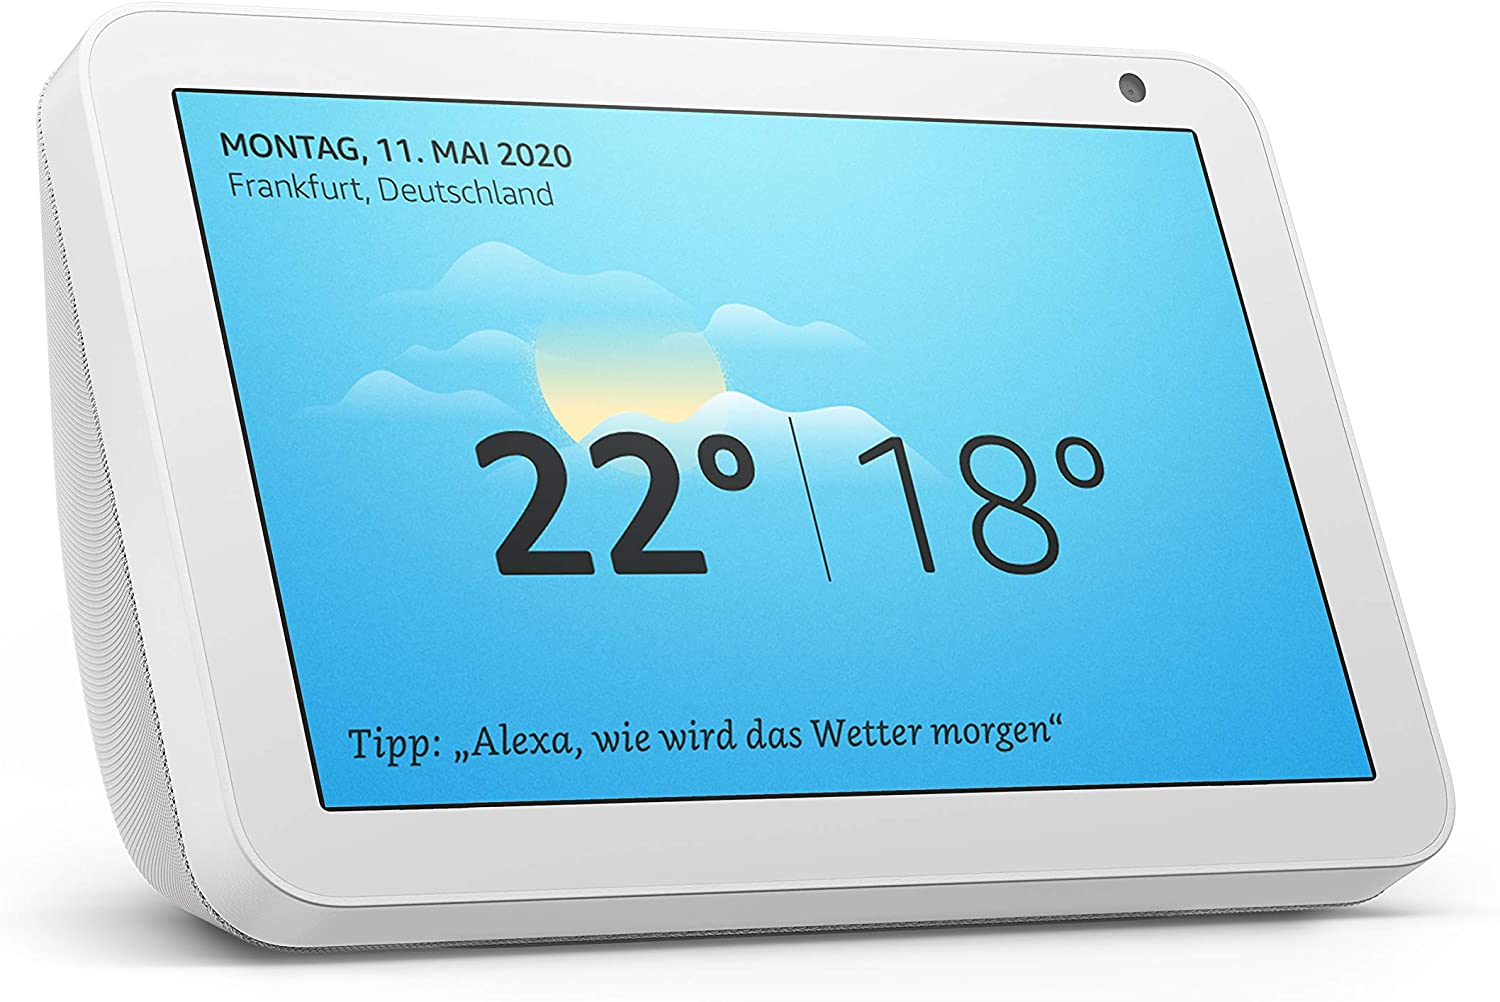
\includegraphics[width=0.9\textwidth]{img/alexa_echo_show8.jpg}
 			\caption[Amazon Alexa Echo Show 8]{Amazon Alexa Echo Show 8}
 			\label{fig:alexa-echo-show8}
 		\end{subfigure}
 		\hfill
 		\begin{subfigure}[t]{0.3\linewidth}
 			\centering
 			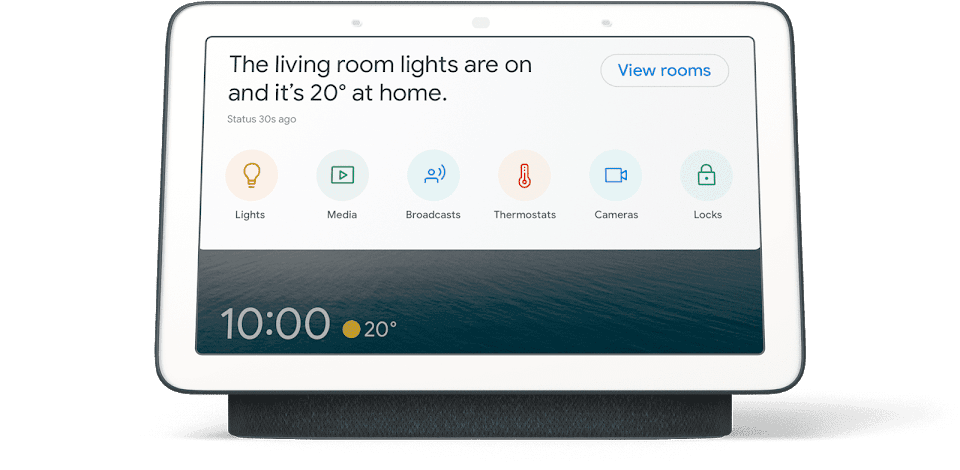
\includegraphics[width=0.9\textwidth]{img/google_nest_hub.png}
 			\caption[Google Nest Hub]{Google Nest Hub}
 			\label{fig:google-nest-hub}
 		\end{subfigure}
 		\hfill
 		\begin{subfigure}[t]{0.3\linewidth}
 			\centering
 			\includegraphics[width=0.9\textwidth]{img/glancr_smart_mirror.jpeg}
 			\caption[Glancr Smart Mirror]{Glancr Smart Mirror}
 			\label{fig:glancr-smart-mirror}
 		\end{subfigure}
 		\caption[Beispiele für Smart Home Zentralen]{Smart Home Zentralen}
 		\label{fig:smart-home-zentralen}
 	\end{figure}
	\textbf{Smart Home Zentralen}, auch \textbf{Smart Hubs} oder \textbf{Smart Mirrors} genannt, sind Geräte, die als zentraler Knotenpunkt in einem Smart Home Netzwerk sitzen und dort Informationen verarbeiten, weiterleiten und darstellen können.\par
 	Diese Geräte werden von den meisten Herstellern mit und ohne Bildschirm geliefert, um entweder ein neues Smart Home aufzubauen oder ein bestehendes Smart Home zu erweitern. 
 	\begin{quote}
 		\color{quotetext}
 		Bei einem Smart-Home-Hub handelt es sich um eine schlaue Zentrale, durch die all deine intelligenten Geräte miteinander vernetzt werden – und dadurch erst wirklich ihren gesamten Leistungsumfang ausschöpfen.\footnote{Li (2017): Was ist ein Smart-Home-Hub? Alles über die intelligente Zentrale}
 	\end{quote}
Als Smart Home Zentrale können auch Software-Lösungen gezählt werden, die mit den im Netz befindlichen Smart Hubs kommunizieren und die Informationen mit Hilfe eines Web-Interfaces oder einer Smartphone-Anbindung darstellen und steuern können. Beispiele hierfür sind homeassistant.io, openHAB und Google Home.\par
% WARUM WILL DAS NIT ANGEZEIGT WERDEN!!!
\begin{figure}[h!tb]
 	\centering
 	\begin{subfigure}[b]{0.3\linewidth}
 		\centering
 		
\includegraphics[width=0.7\textwidth]{img/home-assistant-io_logo.png}
 		\caption[Home Assistant Logo]{Home Assistant}
 		\label{fig:hassio-logo}
 	\end{subfigure}
 	\hfill
 	\begin{subfigure}[b]{0.3\linewidth}
 		\centering
 		
\includegraphics[width=0.7\textwidth]{img/google-cast_logo.png}
 		\caption[Google Home Logo]{Google Home}
 		\label{fig:google-home-logo}
 	\end{subfigure}
 	\hfill
 	\begin{subfigure}[b]{0.3\linewidth}
 		\centering
 		
\includegraphics[width=0.7\textwidth]{img/openhab_logo.png}
 		\caption[openHAB Logo]{openHAB}
 		\label{fig:openhab-logo}
 	\end{subfigure}
 	\caption[Beispiele für Smart Home Software]{Smart Home Software}
 	\label{fig:software-logos}
\end{figure}
% Datenschutzhinweis
\subsection{Datenschutzhinweis}
Aus Datenschutzgründen sind lokale IP-Adressen und lokale Domänennamen innerhalb der Dokumentation unkenntlich gemacht.
\newpage
 	% Zielsetzung
	\section{Zielsetzung}\label{zielsetzung}
Als Ziel für das Projekt war ein funktionsfähiges Smart Home Hub mit Zigbee-Anbindung auf Basis eines Raspberry Pi 4 geplant. Im Laufe des Projekts kam dann noch eine Erweiterungskarte für den Raspberry Pi, ein sog. Raspberry Pi HAT, hinzu, welcher aber aufgrund der vorliegenden Lage mit der COVID-19-Pandemie und den damit verbundenen Liefer- und Zollschwierigkeiten verworfen wurde. Die Planung des HAT ist daher nur rudimentär und nicht vollständig, kann aber bei Bedarf nach Beenden des Projekts durchgeführt werden. Das Smart Home Hub in seiner Grundfunktion soll in der Lage sein, die mit ihm verbundenen Geräte über den Zigbee-Standard anzusteuern. Darüber sollte die Möglichkeit einer Erweiterung mit einem Sprachassistenten gegeben sein.\par
% Konzeption
\subsection{Konzeption}
Zu Beginn des Projekts haben wir uns gemeinsam auf Nachforschung begeben und uns bereits vorhandene Open-Source-Lösungen im Bereich Smart Home angeschaut. Dabei sind wir neben dem Smart Mirror GLANCR auch auf die Gesamtlösung homeassistant.io sowie openHAB gestoßen. Darauf hin haben wir ein Grundkonzept in unserem Lastenheft zusammengefasst und dieses in Absprache mit unserem Betreuungslehrer, Herr Kohler, ausgearbeitet.\par
Nach Abgabe des Lastenhefts haben wir uns dann an die Beschaffung der unserer Meinung nach nötigen Komponenten für das Projekt gemacht.
% Anforderungen und gewünschte Features
\subsection{Anforderungen und gewünschte Features}\label{zs_anforderungen}
Die Anforderungen an das Projekt lauteten demnach wie folgt:
\begin{itemize}
	\item Anbindung von ZigBee-fähigen Endgeräten
	\item Steuerung der angebundenen Endgeräte
	\item Übermittlung der Zustände der angebundenen Geräte an z.B. ein Smartphone
\end{itemize}
Diese Anforderungen lassen sich mit einem Raspberry Pi und einem Zigbee-USB-Stick realisieren. Darüber hinaus waren von unserer Seite noch folgende Features gewünscht:
\begin{itemize}
	\item Ein- und Ausgabe über einen Touch-Bildschirm
	\item Einbindung eines Sprachassistenten zur Steuerung der eingebundenen Endgeräte
\end{itemize}
Nach Fortschritt des Projekts kam bei einer Rücksprache mit unserem Projektbetreuer die Idee auf, einen Raspberry Pi Hat speziell für das Projekt zu entwickeln. Dieser sollte die Hardware des Projekts falls möglich auf einer Platine vereinen, die dann auf den Raspberry Pi aufgesteckt werden konnte.\par
Diese Erweiterungsplatine sollte folgende Eigenschaften besitzen:
\begin{itemize}
	\item ZigBee-Controller und Antenne
	\item NFC-Controller und Antenne
	\item RGB-LED zur Statusanzeige
	\item Anschluss für Lüfter
	\item Sensoren für:
	\begin{itemize}
		 \item Luftfeuchtigkeit
		 \item Temperatur
		 \item Luftdruck
	\end{itemize}
	\item Pins zum Anschluss an Versuchsaufbau für Laborgebrauch
\end{itemize}
Die Erweiterungsplatine wurde aber wie zuvor aufgrund der aktuellen Pandemie-Situation und den damit verbundenen Beschaffungsschwierigkeiten verworfen.
Darauf wurde dann klar, dass eine Erstellung eines Installationsskripts für den Raspberry Pi eine sinnvolle Ergänzung der Projektarbeit wäre. Zusätzlich haben wir ein Gehäuse für die Hardware geplant, um das Endprodukt so wertiger gestalten zu können.
\newpage
	% Herangehensweise
	\section{Herangehensweise}
Nach Festlegung der Anforderungen haben wir uns dann mit der Beschaffung und der Einrichtung der benötigten Materialien gemacht. Hierfür haben wir zum Teil bereits vorhandene Hardware, z.B. den Raspberry Pi 4 mit weiteren Komponenten wie dem Touch-Bildschirm und den Lautsprechern sowie dem Mikrofon ergänzt.
% Hardware
\subsection{Hardware}\label{hgw_hardware}
Bei der Entwicklung der Hardware haben wir für unser Projekt intern einige Rahmenbedinungen festgelegt:
\begin{itemize}
	\item Das Projekt sollte nach Möglichkeit von durchschnittlichen Bastlern durchgeführt werden
	\item Zur Fertigstellung des Projekts sollte mit Handelsüblichen Bastler Werkzeugen möglich sein
	\item Die Grundplattform sollte der 2020 herausgebrachte Raspberry Pi 4 8GB sein\footnote{Wikipedia: Raspberry Pi - Generations}
	\item Das Gerät sollte möglichst von vielen Herstellern vertriebenen Zigbee-Endgeräte verwalten können.
\end{itemize}
\noindent Die Beschaffung der Teile lief dank Online-Versandhandel relativ problemlos. 
Beim Zusammenbau haben wir den Prototyp lediglich mit dem Bildschirm, dem Pi und dem Zigbee-USB-Stick aufgebaut (vgl. Abschnitt \ref{hw_prototype}: \nameref{hw_prototype}). 
Die beiden Standfüße stammen vom Hersteller des Bildschirms Sunfounder \footnote{Sunfounder: 10.1 Inch Touch Screen for Raspberry Pi(NEW) - 3D-printed Touch Screen Support}.
Diese haben wir aus PETG auf dem Ender 3 gedruckt. 
Anschließend haben wir die Softwareseite des Projekts bearbeitet (vgl. Abschnitt \ref{hgw_software}: \nameref{hgw_software} \& Kapitel \ref{software}: \nameref{software}).\par
\noindent Nachdem der Prototyp soweit funktionsfähig war, haben wir uns daran gemacht, das Präsentationsmodell zu entwerfen. 
Dabei ging es uns vornehmlich um die Unterbringung der geplanten Komponenten in einem simplen Gehäuse. 
Hierfür waren einige Verlängerungskabel nötig, um Stromzufuhr, Netzwerk und die Antenne des Zigbee-Sticks nach außen zu leiten (vgl. Abschnitt \ref{hw_case_modellentwicklung}: \nameref{hw_case_modellentwicklung} \& Abschnitt \ref{ku_produkt}: \nameref{ku_produkt}). \\
\noindent Das Gehäuse wurde dann nach dem Druck mit dem Bildschirm verklebt und die einzelnen Komponenten verbaut (vgl. Abschnitt \ref{hw_case_herstellung}: \nameref{hw_case_herstellung}). 
Nachdem das Gerät soweit fertig war, haben wir einen Versuchsaufbau zur Präsentation aufgebaut, der die Funktionsweise des Geräts in einem ,,typischen'' Heimnetzwerk darstellen soll (vgl. Abschnitt \ref{hw_testaufbau}: \nameref{hw_testaufbau}).\\
\noindent Näheres zur Herangehensweise im Kapitel \ref{hardware}: \nameref{hardware}.
% Software
\subsection{Software}\label{hgw_software}
\newpage
	% Zeitplan
	\section{Zeitplan}\label{zeitplan}
\begin{figure}[H]
	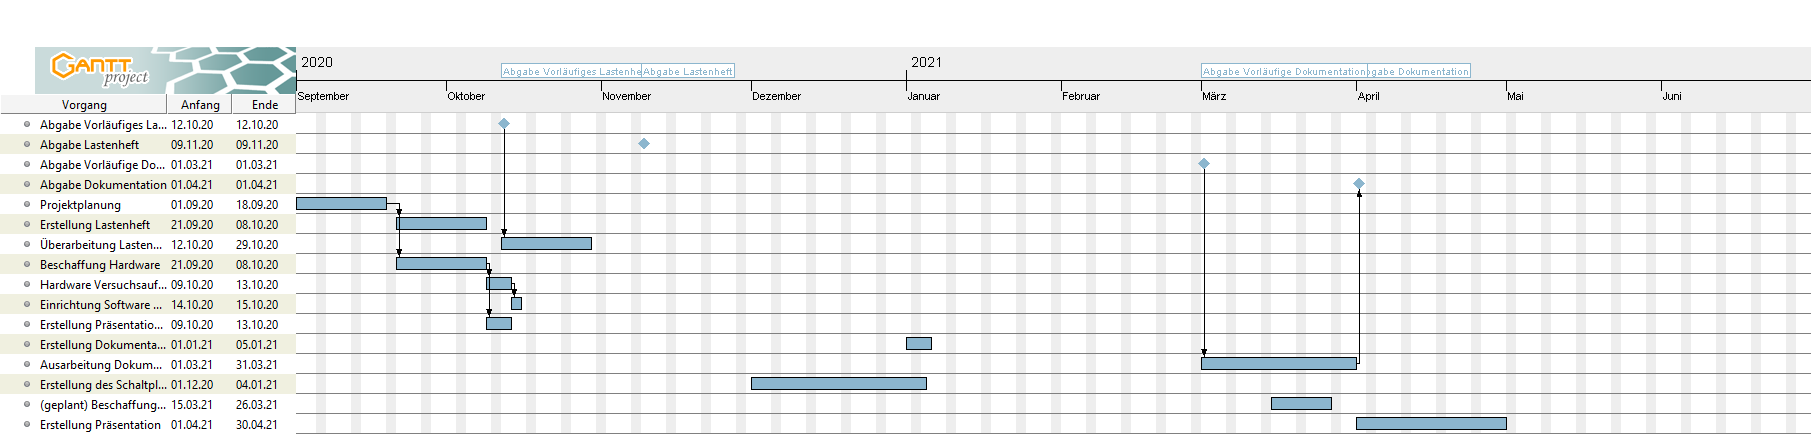
\includegraphics[width=1\textwidth]{img/TAR_FKMS_20202021.png}
	\caption[gantt-Diagramm des Projektablaufs]{gantt-Diagramm des Projektablaufs}
 	\label{fig:gantt-diagramm}
\end{figure}
Um einen besseren Überblick der Aufgaben zu haben, haben wir mit GanttProject ein Gantt-Diagramm mit den Aufgaben und Meilensteinen unseres Projekts angelegt (vgl. Abb. \ref{fig:gantt-diagramm}: \nameref{fig:gantt-diagramm}).
Die eigentliche Projektorganisation war als SCRUM Projekt geplant. Hierfür haben wir das KANBAN-Board in Microsoft Teams genutzt (vgl. Abb \ref{fig:kanban}: \nameref{fig_kanban}).
Dadurch haben wir stets einen Überblick über die noch zu erledigenden, offenen und erledigten Aufgaben.\\
\begin{figure}[H]
    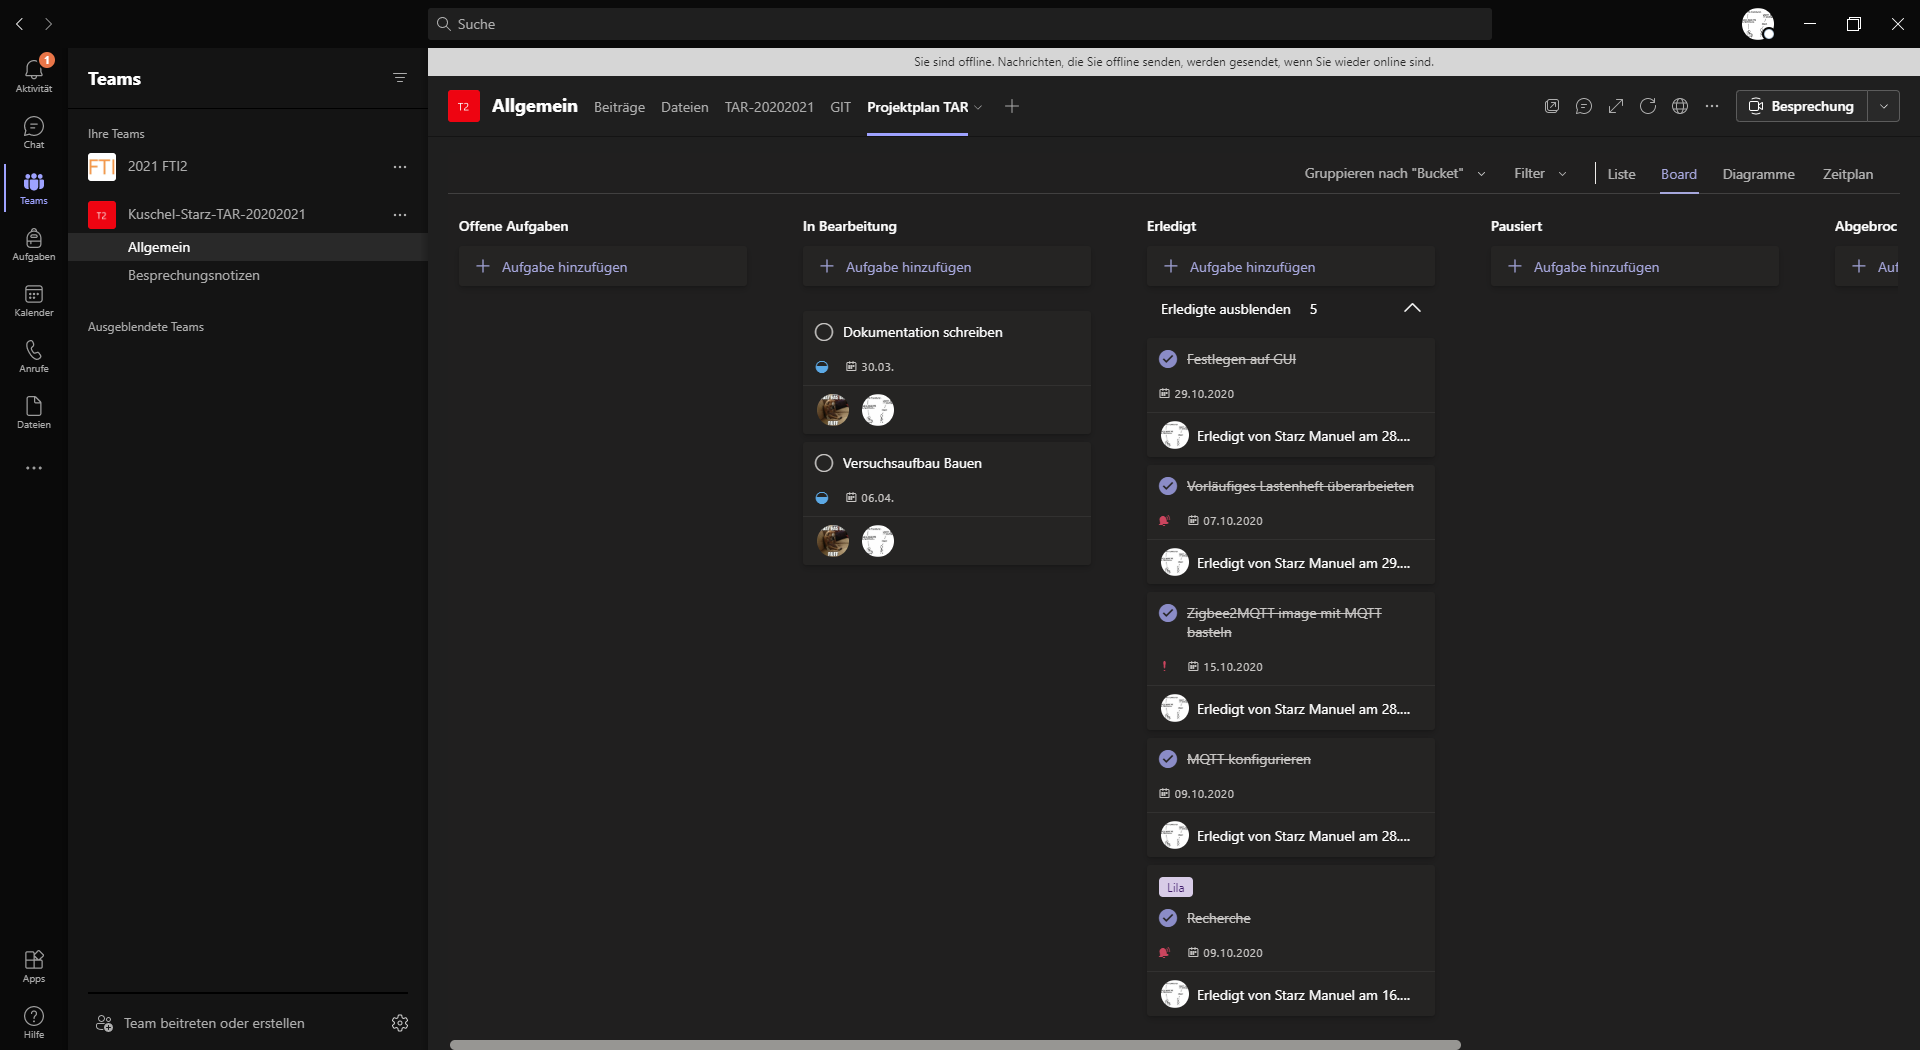
\includegraphics[width=1\textwidth]{img/teams_kanban.png}
    \caption[KANBAN-Board in Microsoft Teams]{KANBAN-Board in Microsoft Teams}
    \label{fig:kanban}
\end{figure}
\noindent Microsoft Teams hat uns auch als Kommunikationsplattform während der Lockdown-Zeiten. 
Dadurch konnten wir während der üblichen Zeiten mit Herr Kohler in Verbindung treten.
\newpage
	% Komplettübersicht
	\section{Komplettübersicht}
%Füllen ;)
\newpage
	% Hardware
	\section{Hardware}\label{hardware}
% Raspberry Pi 4
\subsection{Raspberry Pi 4}\label{hw_raspberrypi}
Als Basis für die Smart Home Zentrale haben wir einen Raspberry Pi in der Version 4 mit 8 GB gewählt, um als von anderen Servern unabhängige Plattform agieren zu können. 
Der Raspberry Pi 4 ist mit einem ARM Cortex-A72 Prozessor ausgestattet, der über 4 Kerne verfügt.
Zusätzlich hat der Raspberry Pi 4 über einen Gigabit-Netzanschluss.
In der Makerszene ist der Raspberry Pi weit verbreitet und dient bei anspruchsvolleren Projekten als Kern.\par
\begin{quote}
 		\color{quotetext}
 		Der Raspberry Pi hat sich seit der ersten Veröffentlichung Anfang 2012 weltweit schon millionenfach verkauft und erfreut sich immer noch größter Beliebtheit. Denn viele Raspberry Pi User haben nicht nur einen Einplatinen-Computer zu Hause, sondern teils 4-5 Stück.
Der eine fungiert als HD-Mediaplayer mit externer Festplatte für das heimische Kino oder als Internetradio mit Display, der nächste als Webcam-Server für die Kameraüberwachung mit Livestream auf das Handy, dann noch einer für die Hausautomatisierung wie bspw. die Heizungs- oder Lichtsteuerung und noch einer als einfacher WLAN-Druckerserver oder als Mini-Computer zum allgemeinen Surfen im Internet, um ein paar wenige Anwendungsszenarien zu nennen.
Sie merken, der kleine ,,Tausendsassa'' kann nicht nur viel, sondern ist zudem auch noch extrem günstig und eben das macht den Reiz aus. Lediglich den Hang zum Programmieren sollten Sie mitbringen und selbst nicht mal das, denn Sie können auch einfach nach Anleitung aus Foren oder Büchern nachprogrammieren, oder ganz bequem ein fertiges Image auf den Raspberry Pi installieren - trauen Sie sich! 
\footnote{reichelt.de: Produktbeschreibung des Raspberry Pi 4}
\end{quote}
\newpage
\par
% Aufbau des Prototypen
\subsection{Aufbau des Prototypen}\label{hw_prototype}
Der Prototyp war eine Kombination aus dem verwendeten Touchscreen sowie dem Raspberry Pi 4 und dem Zigbee-Stick. Dieser Prototyp diente als Entwicklungsplattform für die Software.
\begin{figure}[h!tb]
	\begin{subfigure}[b]{0.5\linewidth}
		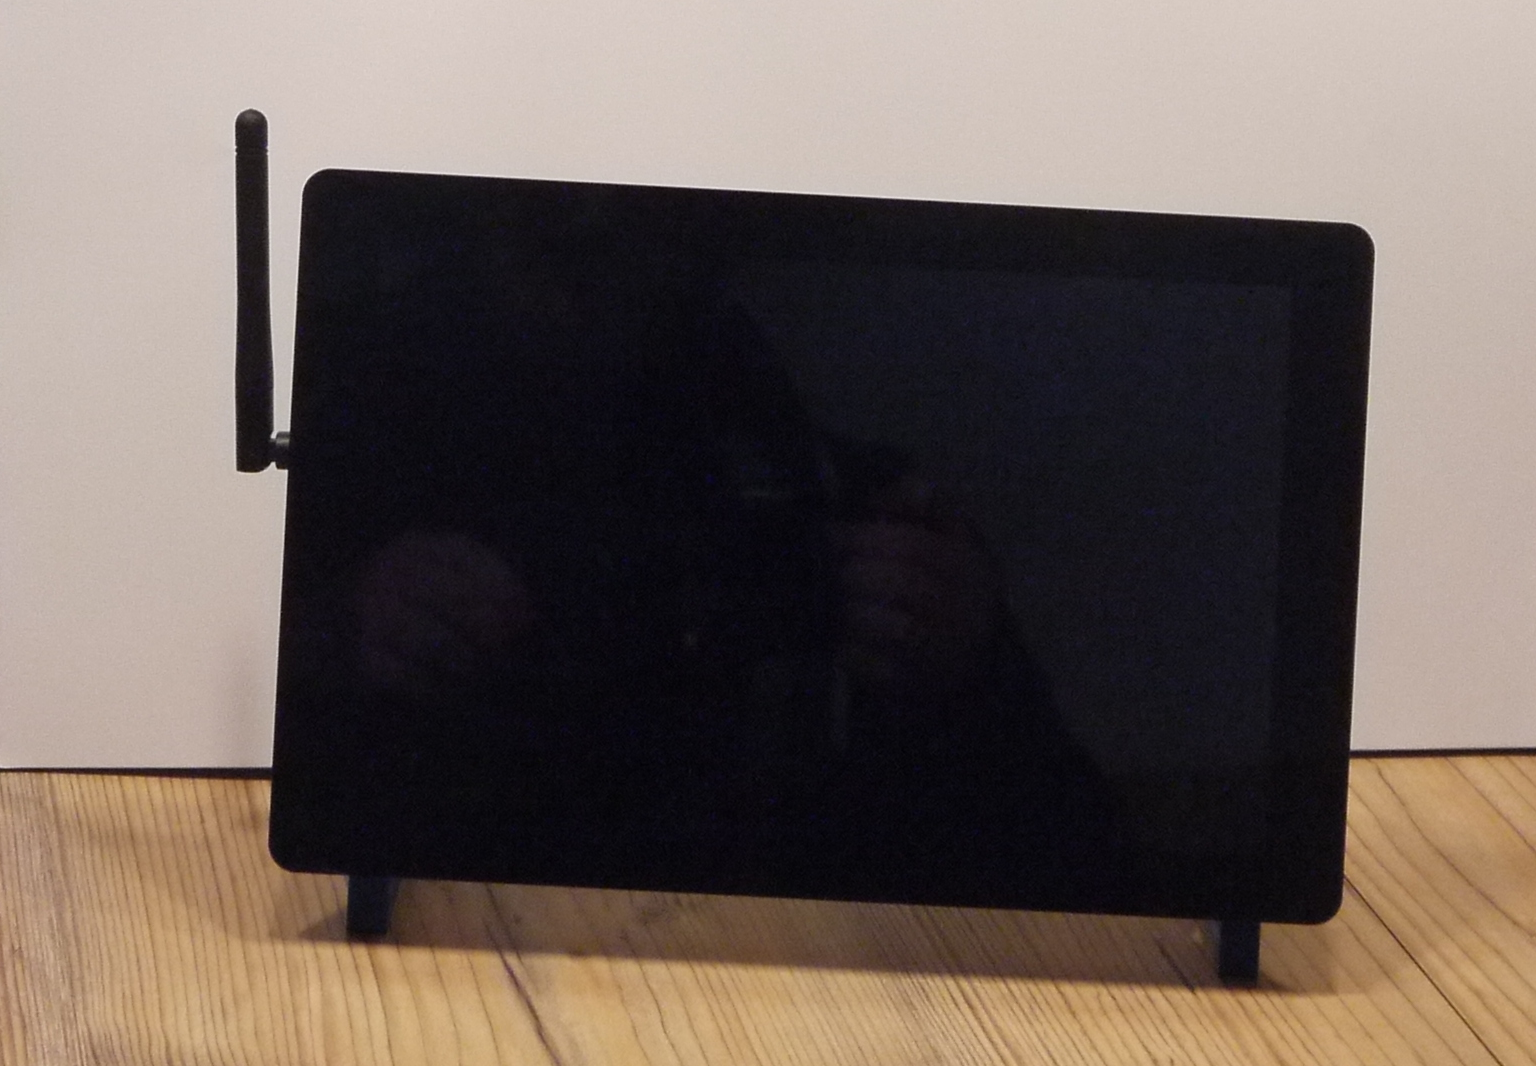
\includegraphics[width=1\textwidth]{img/prototype_front.png}
		\caption[Vorderseite des Prototypen]{Vorderseite des Prototypen}
	\end{subfigure}
	\begin{subfigure}[b]{0.5\linewidth}
		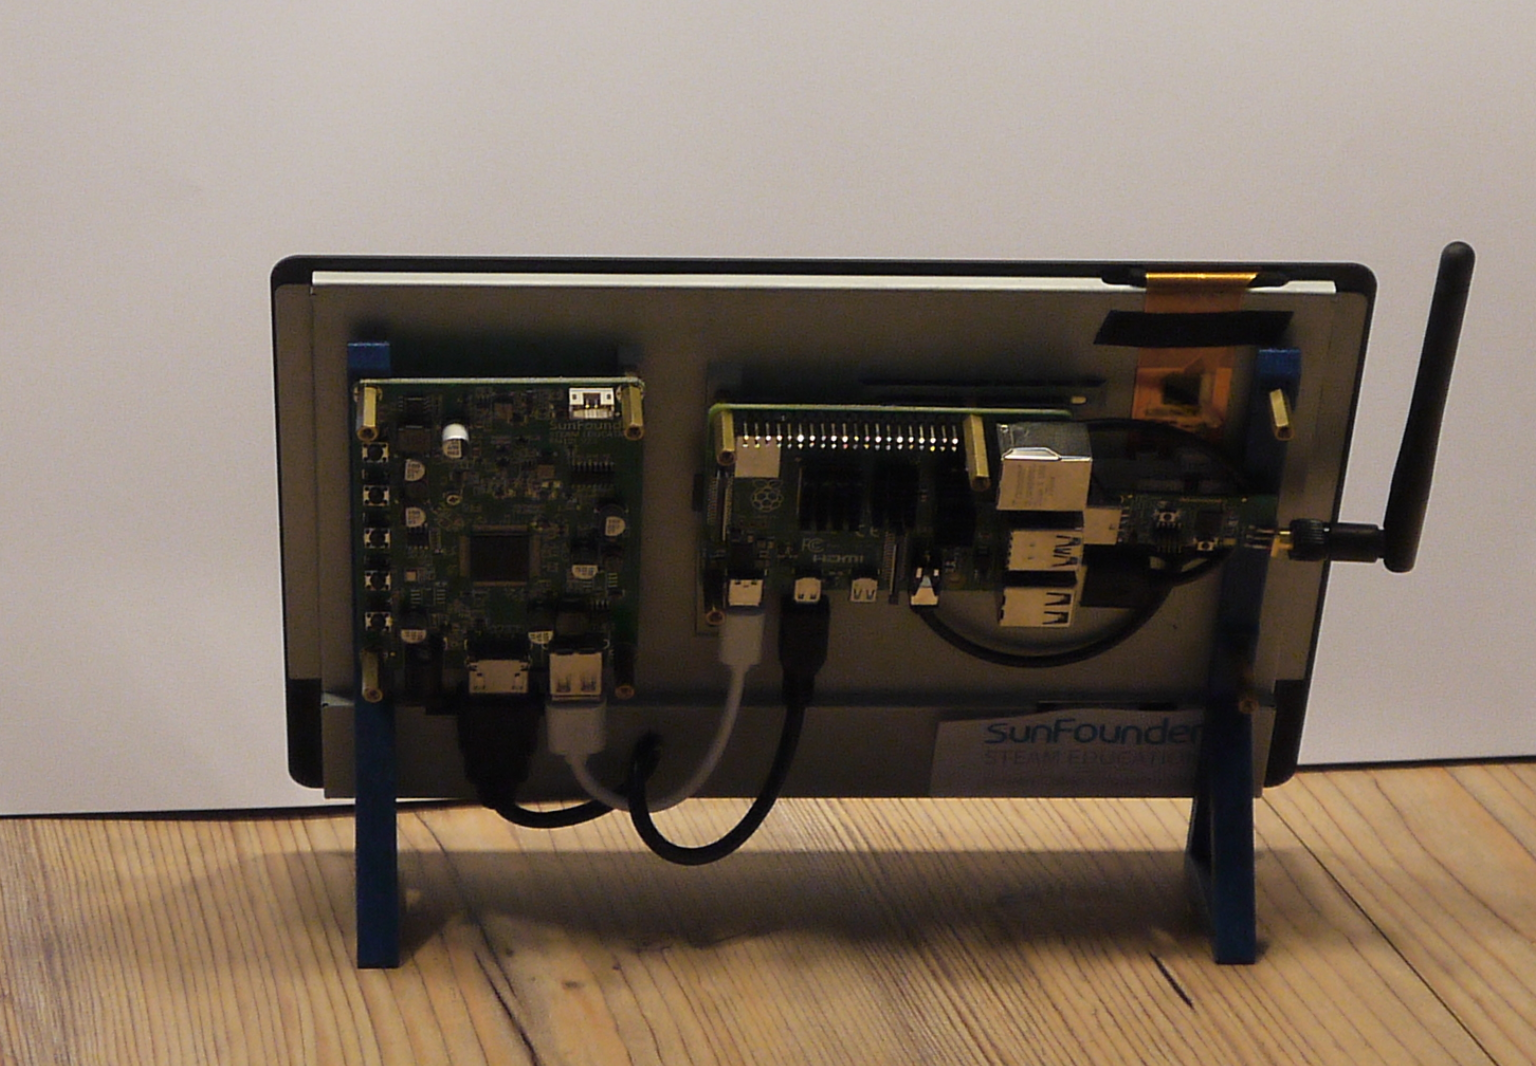
\includegraphics[width=1\textwidth]{img/prototype_back.png}
		\caption[Rückseiteseite des Prototypen]{Rückseite des Prototypen}
	\end{subfigure}
	\begin{subfigure}[b]{1\linewidth}
		\includegraphics[width=1\textwidth]{img/prototype_back_detail.png}
		\caption[Detailansicht der Rückseite]{Detailansicht der Rückseite}
	\end{subfigure}
	\caption[Prototyp der Smart Home Zentrale]{Prototyp der Smart Home Zentrale}
	\label{prototype}
\end{figure}
\newpage
\par
% Gehäuse
\subsection{Gehäuse}\label{hw_case}
% Erster Test
\subsubsection{Erster Test des Gehäuses}
Zur Erstellung des Gehäuses haben wir die Maße des Bildschirms als Anhaltspunkt genommen. Das Gehäuse befand sich zu diesem Zeitpunkt bei Felix Kuschel, der die Messungen vornahm. Der Bildschirm hatte an der Hinterseite eine Erhebung, weshalb er diese ebenfalls ausgemessen hatte. Die Maße beliefen sich dann auf:
\begin{itemize}
	\item 255,5 mm Breite
	\item 167 mm Höhe
	\item Kantenradius 10 mm
\end{itemize}
	\begin{figure}[h!t]
		\includegraphics[width=1\textwidth]{img/abmessungen_gehäuse.jpg}
		\caption[Abmessungen Bildschirm Rückseite]{Abmessungen Bildschirm Rückseite}
		\label{fig:screen-back-01}
	\end{figure}
	Die Maße an der Rückseite übermittelte er Manuel Starz als Bild. Anhand dieser Maße hat Manuel Starz dann in Fusion 360 eine Grundplanzeichnung erstellt und ein 3D-Modell gefertigt.\par	
	Nach Überprüfung der Maße mussten wir dann allerdings feststellen, dass der zur Verfügung stehende 3D-Drucker, ein Ender 3 Pro der Firma Creality3D, ein maximales Druckvolumen von 235x235x220mm besitzt und somit das Gehäuse nicht wie ursrpünglich geplant aus einem Stück sondern in mehreren Teilen gedruckt werden musste. Hierfür war eine Änderung der Konstruktion von Nöten. Das Gehäuse besteht nun aus vier Teilen, zwei bilden jeweils die Seitenwände während zwei den Deckel des Gehäuses bilden. Die Teile werden mit langen M3 Senkkopfschrauben verbunden, die zusätzlich als Verschluss des Gehäuses dient. \par
	
	\begin{figure}[h!]
		\includegraphics[width=1\textwidth]{img/druck_gehäuse_001.png}
		\caption[Platzierung der beiden Gehäusewände in CURA]{Platzierung der beiden Gehäusewände in CURA}
		\label{fig:print-case-test_01}
	\end{figure}
	\begin{figure}[h!]
		\includegraphics[width=1\textwidth]{img/druck_gehäuse_002.png}
		\caption[Verschiebung der Modelle entlang der Z-Achse um 45mm]{Verschiebung der Modelle entlang der Z-Achse um 45mm}
		\label{fig:print-case-test_02}
	\end{figure}
	\begin{figure}[h!]
		\includegraphics[width=1\textwidth]{img/druck_gehäuse_002.png}
		\caption[Slicen der Modelle]{Slicen der Modelle}
		\label{fig:print-case-test_03}
	\end{figure}
	\begin{figure}[h!]
		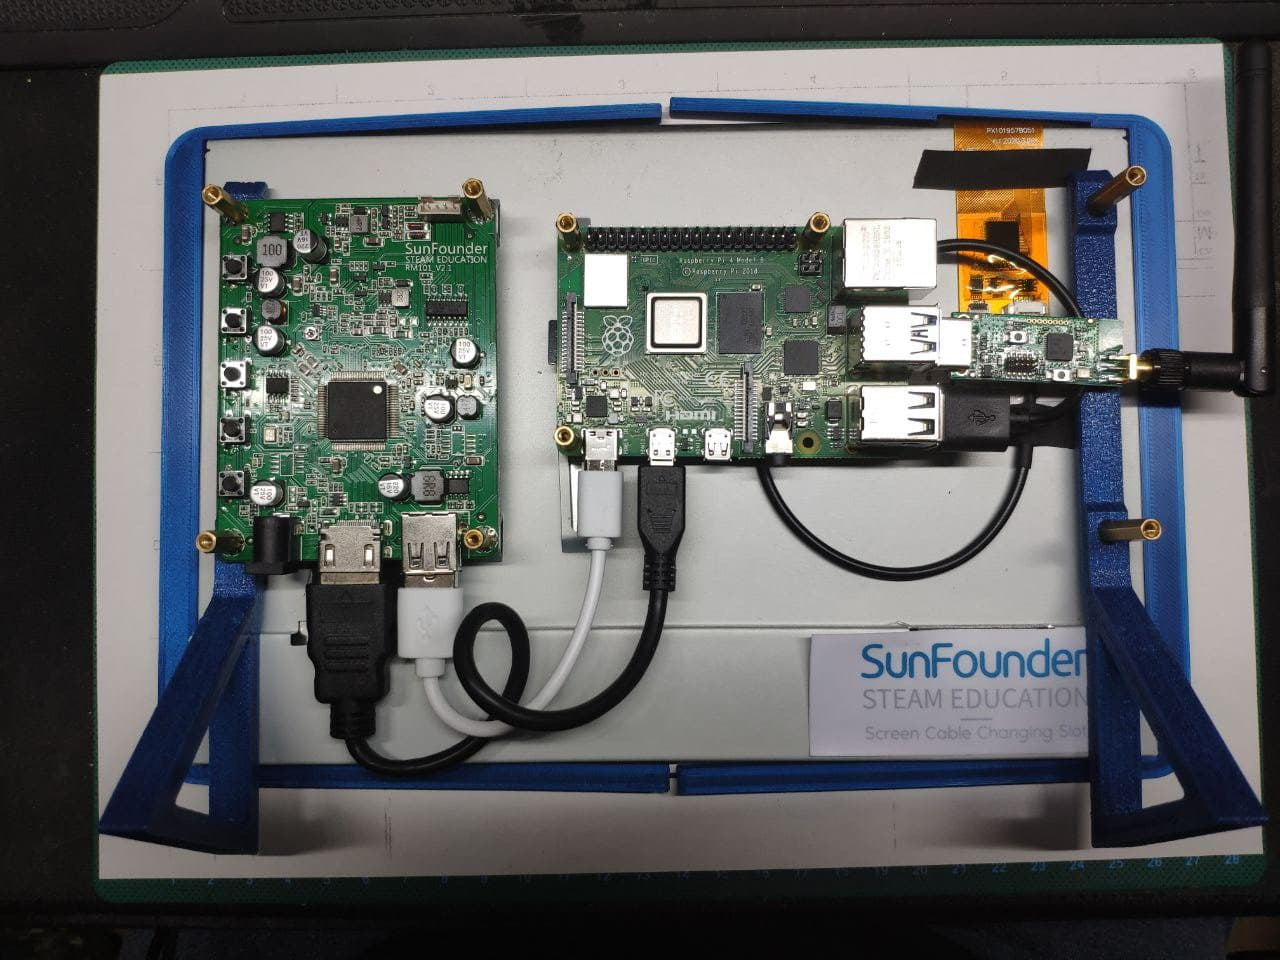
\includegraphics[width=1\textwidth]{img/testdruck_an_bildschirm.jpg}
		\caption[Passung des Testdrucks]{Passung des Testdrucks}
		\label{fig:print-case-test_04}
	\end{figure}
	Um die Genauigkeit der Konstruktion zu testen, hat Manuel Starz eine 5 Millimeter hohe Testschablone ausgedruckt, die an den Bildschirm angelegt werden kann. Diese entstand mit Hilfe des Slicers CURA (vgl. Abbildung \ref{fig:print-case-test_01}), in dem die Modelle der beiden Seitenteile so angeordnet wurden, dass lediglich 5 Millimeter des Teils im druckbaren Bereich des Druckers verblieben (vgl. Abbildung \ref{fig:print-case-test_02}).\par
% Modellentwicklung am Objekt
\subsubsection{Modellentwicklung am Objekt}\label{hw_case_modellentwicklung}
\paragraph{Grundskizze}
Nachdem das Testmodell (vgl. Abbildung \ref{fig:print-case-test_04}) nicht zu 100 \% gepasst hat, hat Manuel Starz die Abmessungen neu geklärt und diese in Fusion 360 übertragen (vgl. \ref{fig:case_footprint}). Um Material für den 3D-Druck zu sparen, wurde die Zeichnung dann im Maßstab 1:1 auf Papier gedruckt, ausgeschnitten und angelegt.\par
Da hier einige Maße noch nicht gestimmt haben, hat Manuel Starz den Plan überarbeitet (vgl. \ref{fig:case_footprint_final}). Diese neuen Bemaßungen waren dann korrekt.\par
Daraufhin wurde dann die Zeichnung in zwei eigenständige Dateien gesplittet, um die linke und die rechte Seite des Gehäuses zu konstruieren.\par
Die Grundabmessung des Bildschirms werden in Fusion 360 als neue Zeichnung angelegt. Hierzu wurde ein einfaches Rechteck mit den entsprechenden Außenmaßen angelegt (vlg. \ref{fig:design-case-01}). Anschließend wurden die Ecken mit einem Radius von 7mm abgerundet. (vgl. \ref{fig:design-case-02}). Abschließend wurde die Zeichnung in der Mitte geteilt, um die beiden Hälften des Gehäuses unabhängig von einander zu konstruieren.\par
\begin{figure}[h!tb]
	\begin{subfigure}[b]{.5\linewidth}
		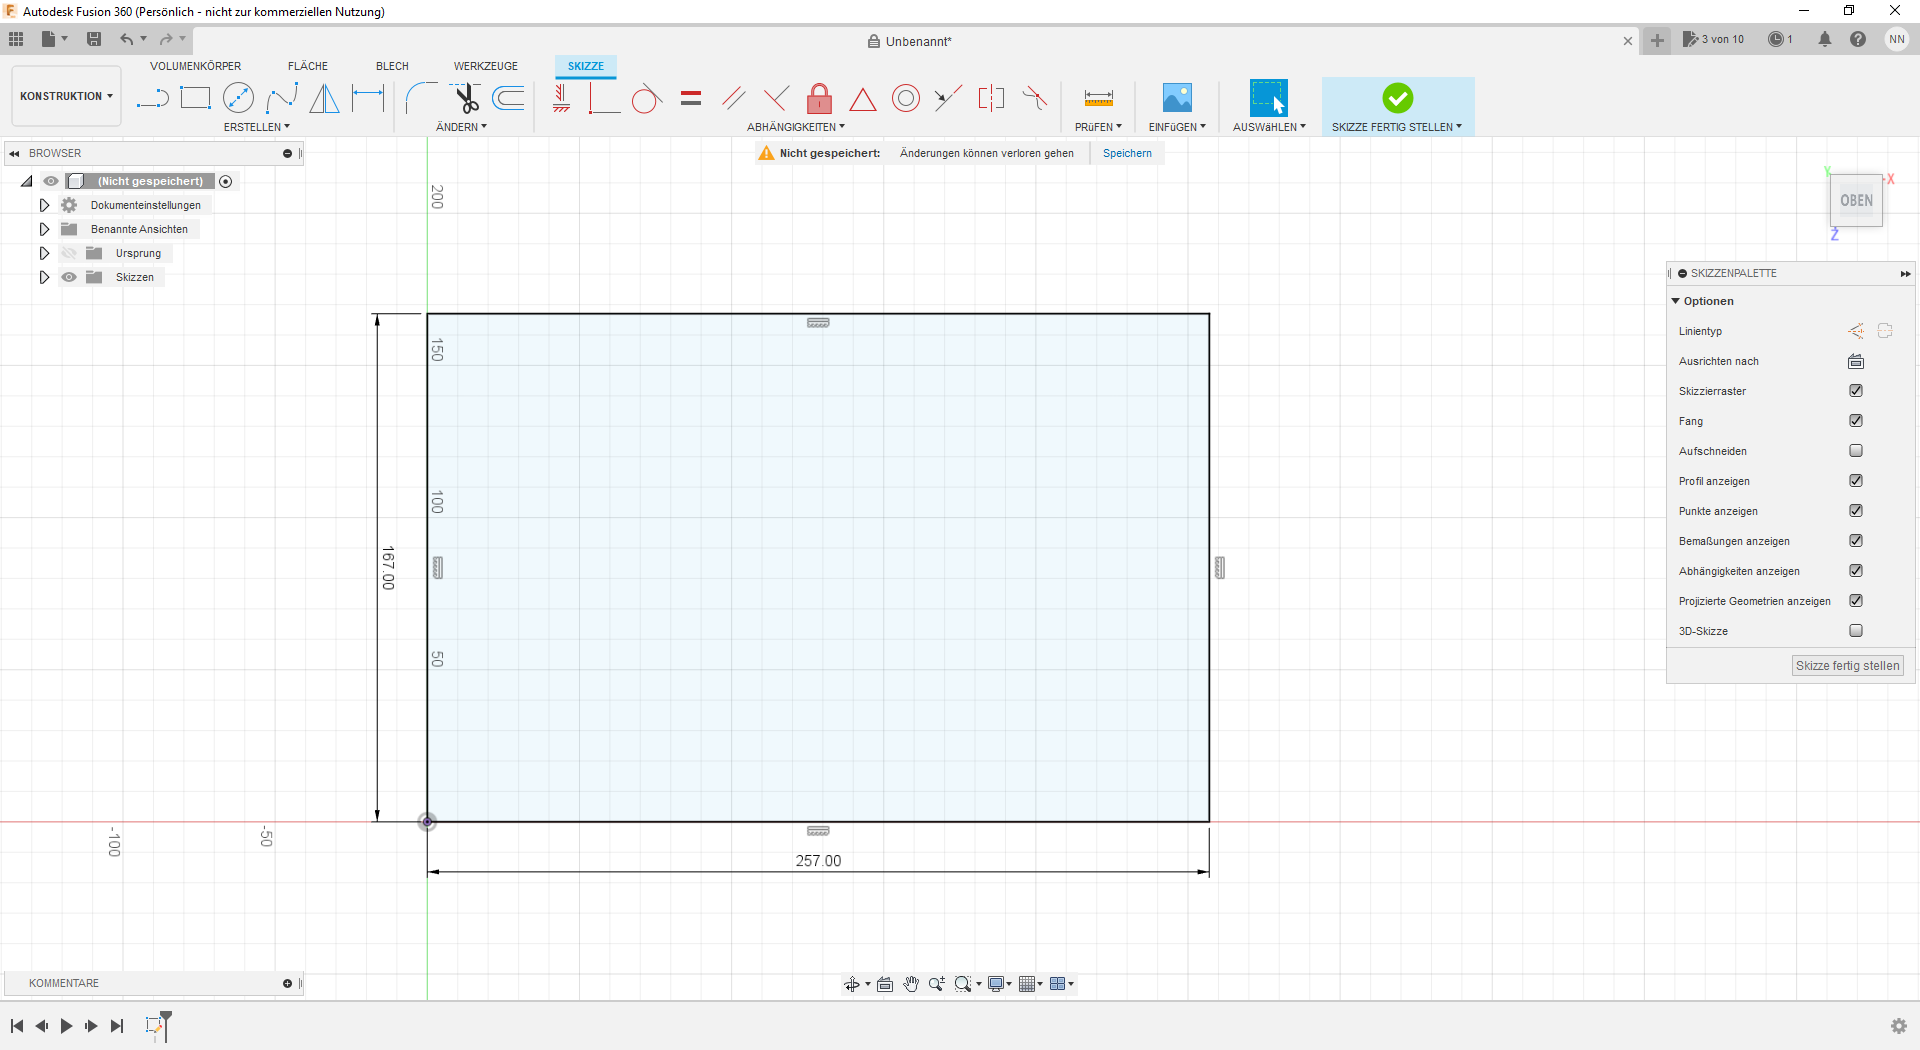
\includegraphics[width=1\textwidth]{img/konstruktion_gehaeuse_001.png}
		\caption[Zeichnen der Außenmaße]{Zeichnen der Außenmaße}
		\label{fig:design-case-01}
	\end{subfigure}
	\begin{subfigure}[b]{.5\linewidth}
		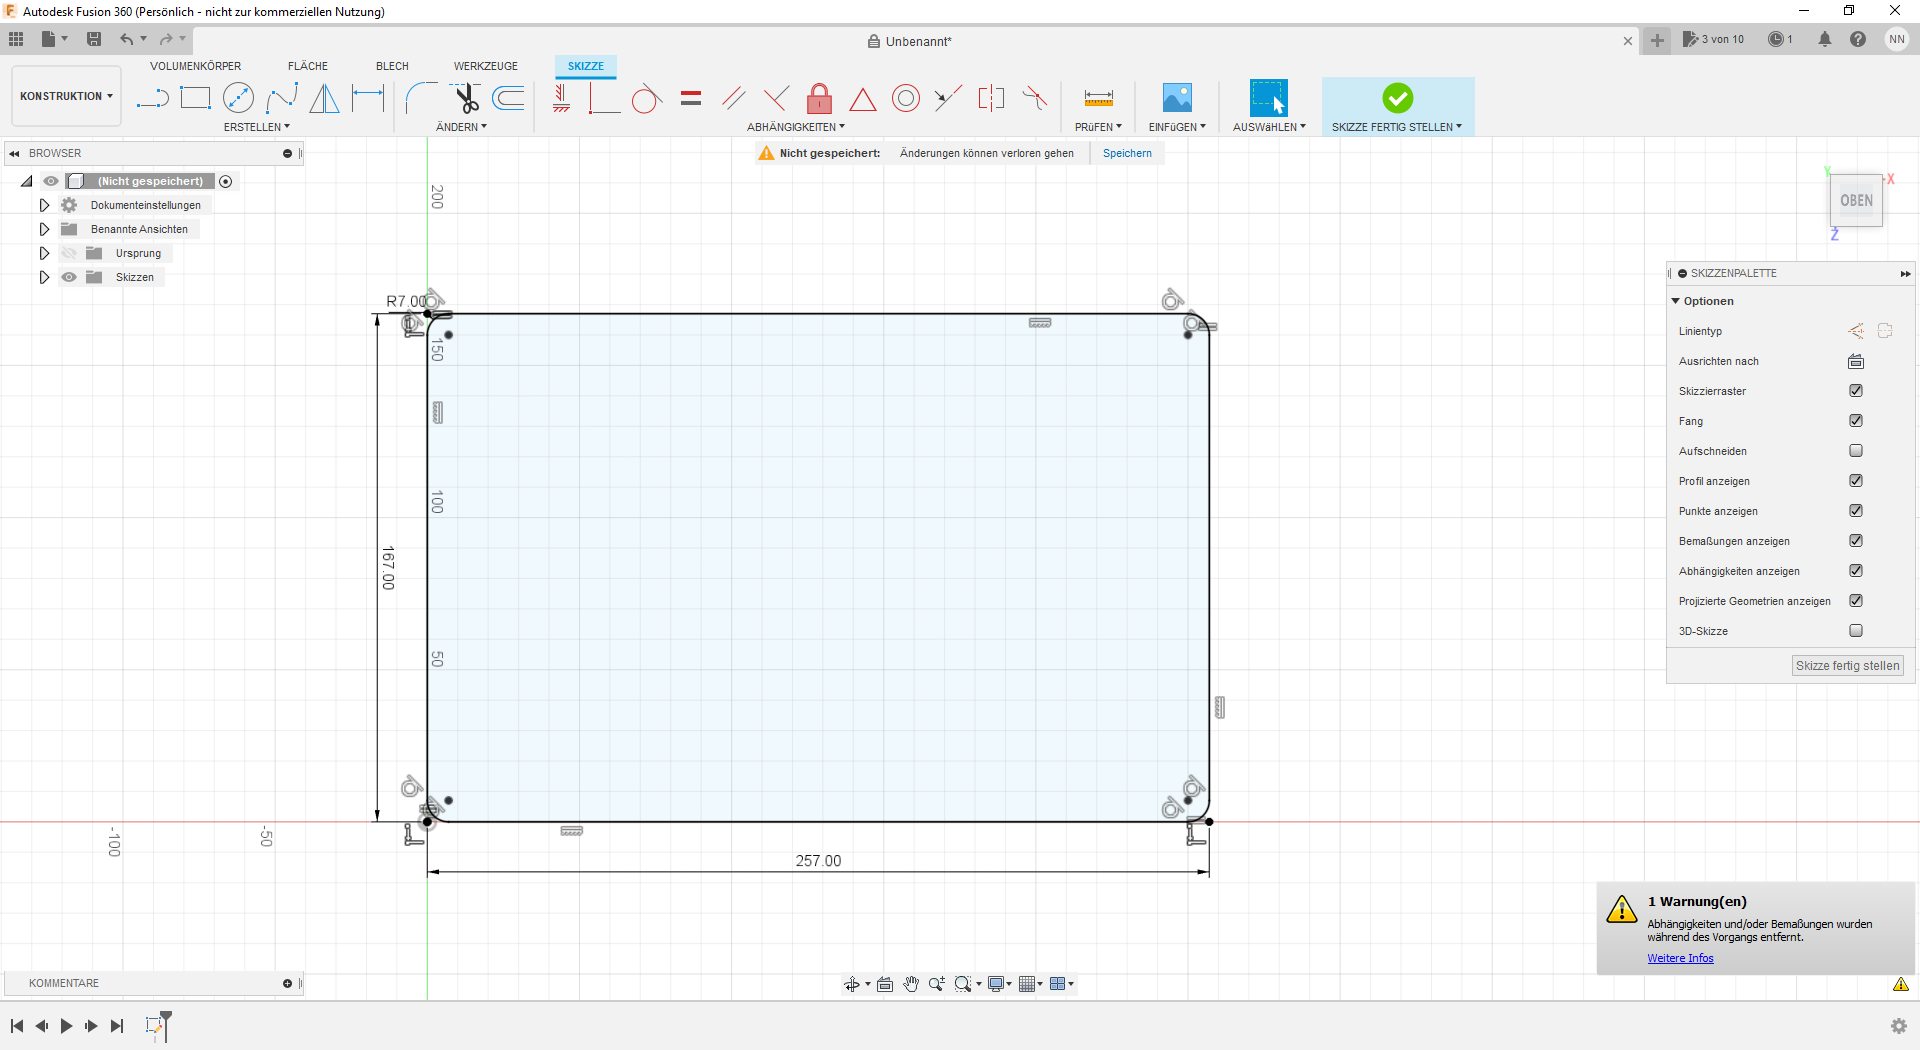
\includegraphics[width=1\textwidth]{img/konstruktion_gehaeuse_002.png}
		\caption[Abrunden der Ecken]{Abrunden der Ecken}
		\label{fig:design-case-02}
	\end{subfigure}
	\begin{subfigure}[b]{.5\linewidth}
		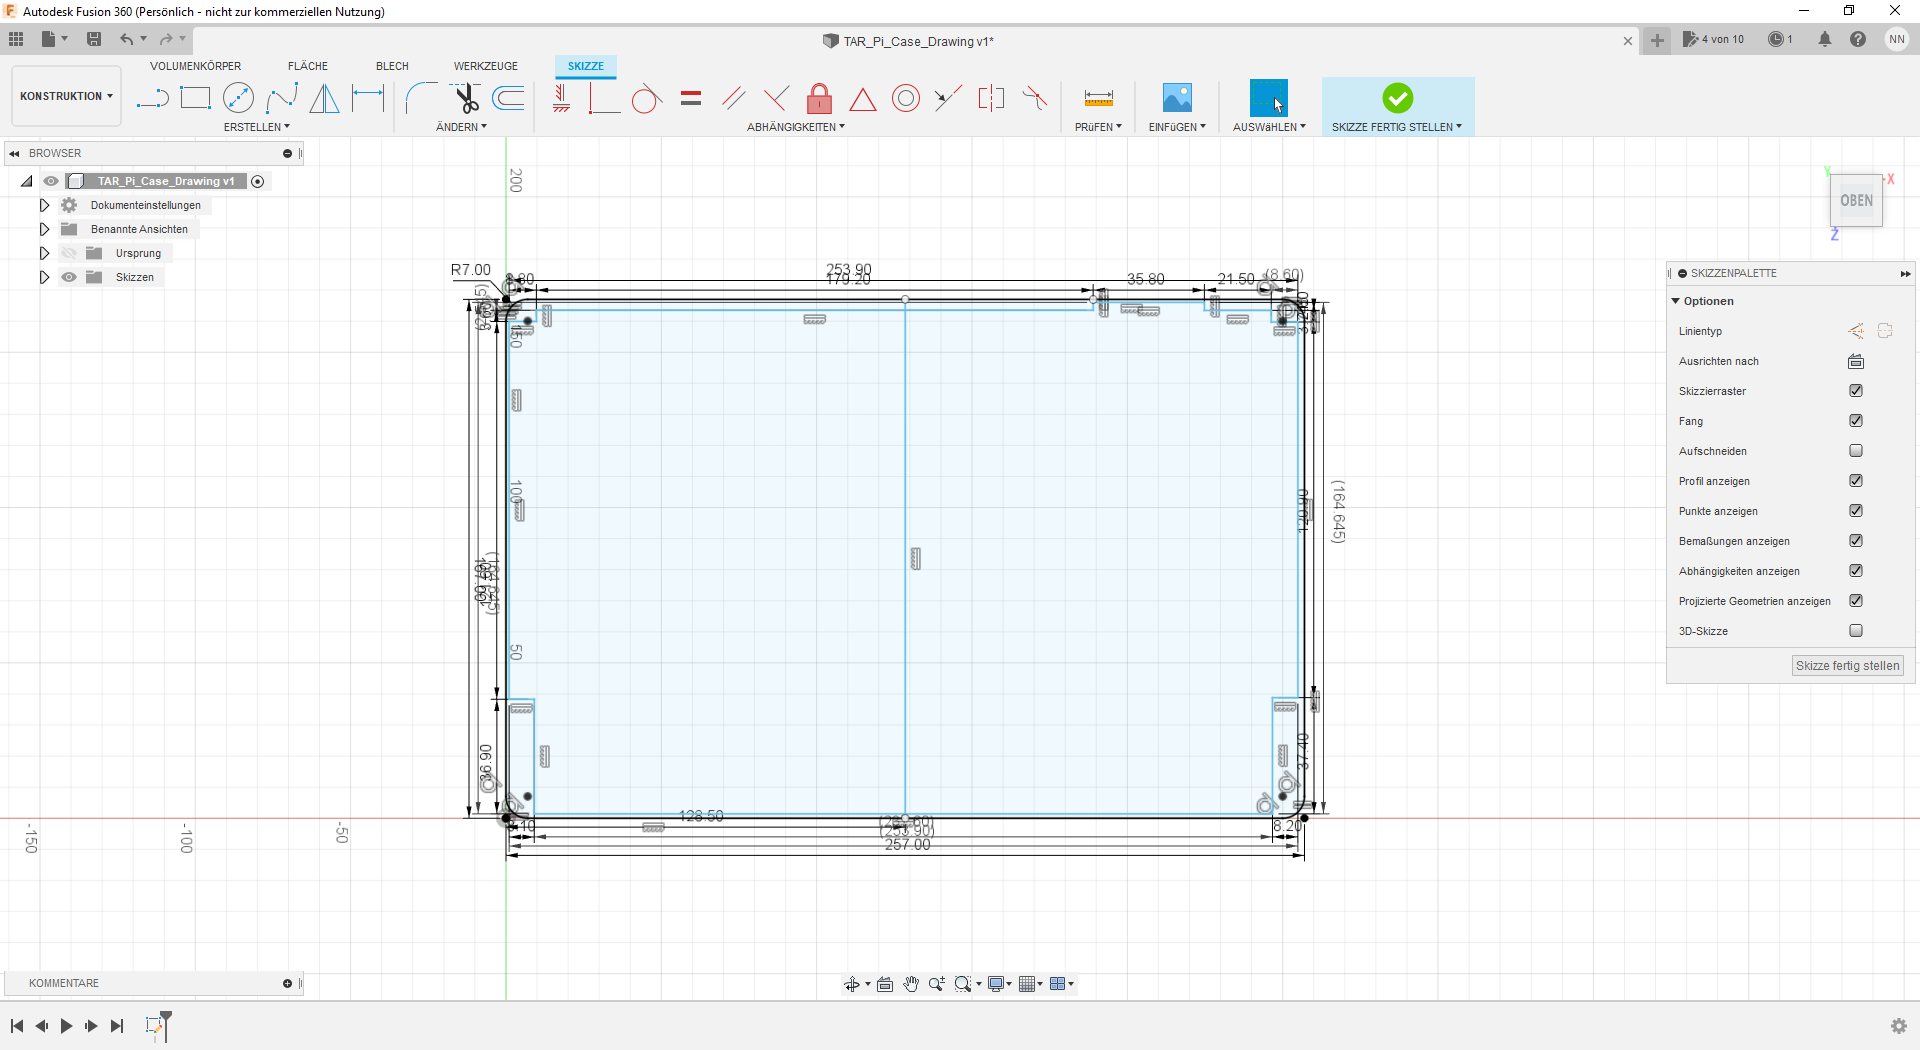
\includegraphics[width=1\textwidth]{img/konstruktion_gehaeuse_003.png}
		\caption[Zeichnen der Auflageflächen für das Gehäuse]{Zeichnen der Auflageflächen}
		\label{fig:design-case-03}
	\end{subfigure}
	\caption[Grundzeichnung als Basis des Modells]{Grundzeichnung als Basis des Modells}
	\label{fig:design-case-base}
\end{figure}\par
Die so entstandene Zeichnung (vgl. \ref{fig:design-case-03}) wurde dann in eine weitere Datei kopiert um als Grundlage für die beiden geteilten Seitenteile zu dienen. Von hier aus wurden die beiden Wand-Teile mehr oder weniger unabhängig voneinander entworfen.\par
\paragraph{Linkes Wandteil}
Beim linken Wandteil wurde der entsprechende Teil der Zeichnung um 2 mm entlang der Z-Achse extrudiert (vgl. \ref{fig:design-left-01}). Auf der erhöhten Seite wurde darauf hin eine weitere Zeichnung gelegt, die die Bleche an der Rückseite des Bildschirms überdecken sollte (vgl. \ref{fig:design-left-02}), die dann wie zuvor um 3 mm entlang der Z-Achse extrudiert wurde (vgl. \ref{fig:design-left-03}). Diese sollte dem Gehäuse genug Auflagefläche an dem Bildschirm bieten, um die Verklebung so stark wie möglich zu machen. Auf die nun entstandene erhöhte Seite wurde eine Zeichnung der ,,tatsächlichen'' Wandstärke von 3 mm erstellt (vgl. \ref{fig:design-left-04}). Diese wurde dann um 6 mm entlang der Z-Achse extrudiert, um für die Verbinder genügend Platz vor dem klobigen Blechbereich im unteren Teil des Bildschirms zu bieten (vgl. \ref{fig:design-left-05}). Auf die nun obenliegende Seite wurde die Zeichnung der Verbindungsstücke gelegt (vgl. \ref{fig:design-left-06}) und um 19 mm entlang der Z-Achse extrudiert (vgl. \ref{fig:design-left-07}) und im Kreismittelpunkt der Zeichnungen eine Bohrung für M3-Gewinde gesetzt (vgl. \ref{fig:design-left-08}). Auf die nun  entstandene Oberfläche wurde die Zeichnung für die Deckelverbindung gesetzt (vgl. \ref{fig:design-left-09}), um 25 mm entlang der Z-Achse extrudiert (vgl. \ref{fig:design-left-10}) und ebenfalls mit Bohrungen für M3-Gewinde versehen (vgl. \ref{fig:design-left-11}).\\
%beschreibungstext links
\begin{figure}[h!tb]
	\begin{subfigure}[t]{.3\linewidth}
		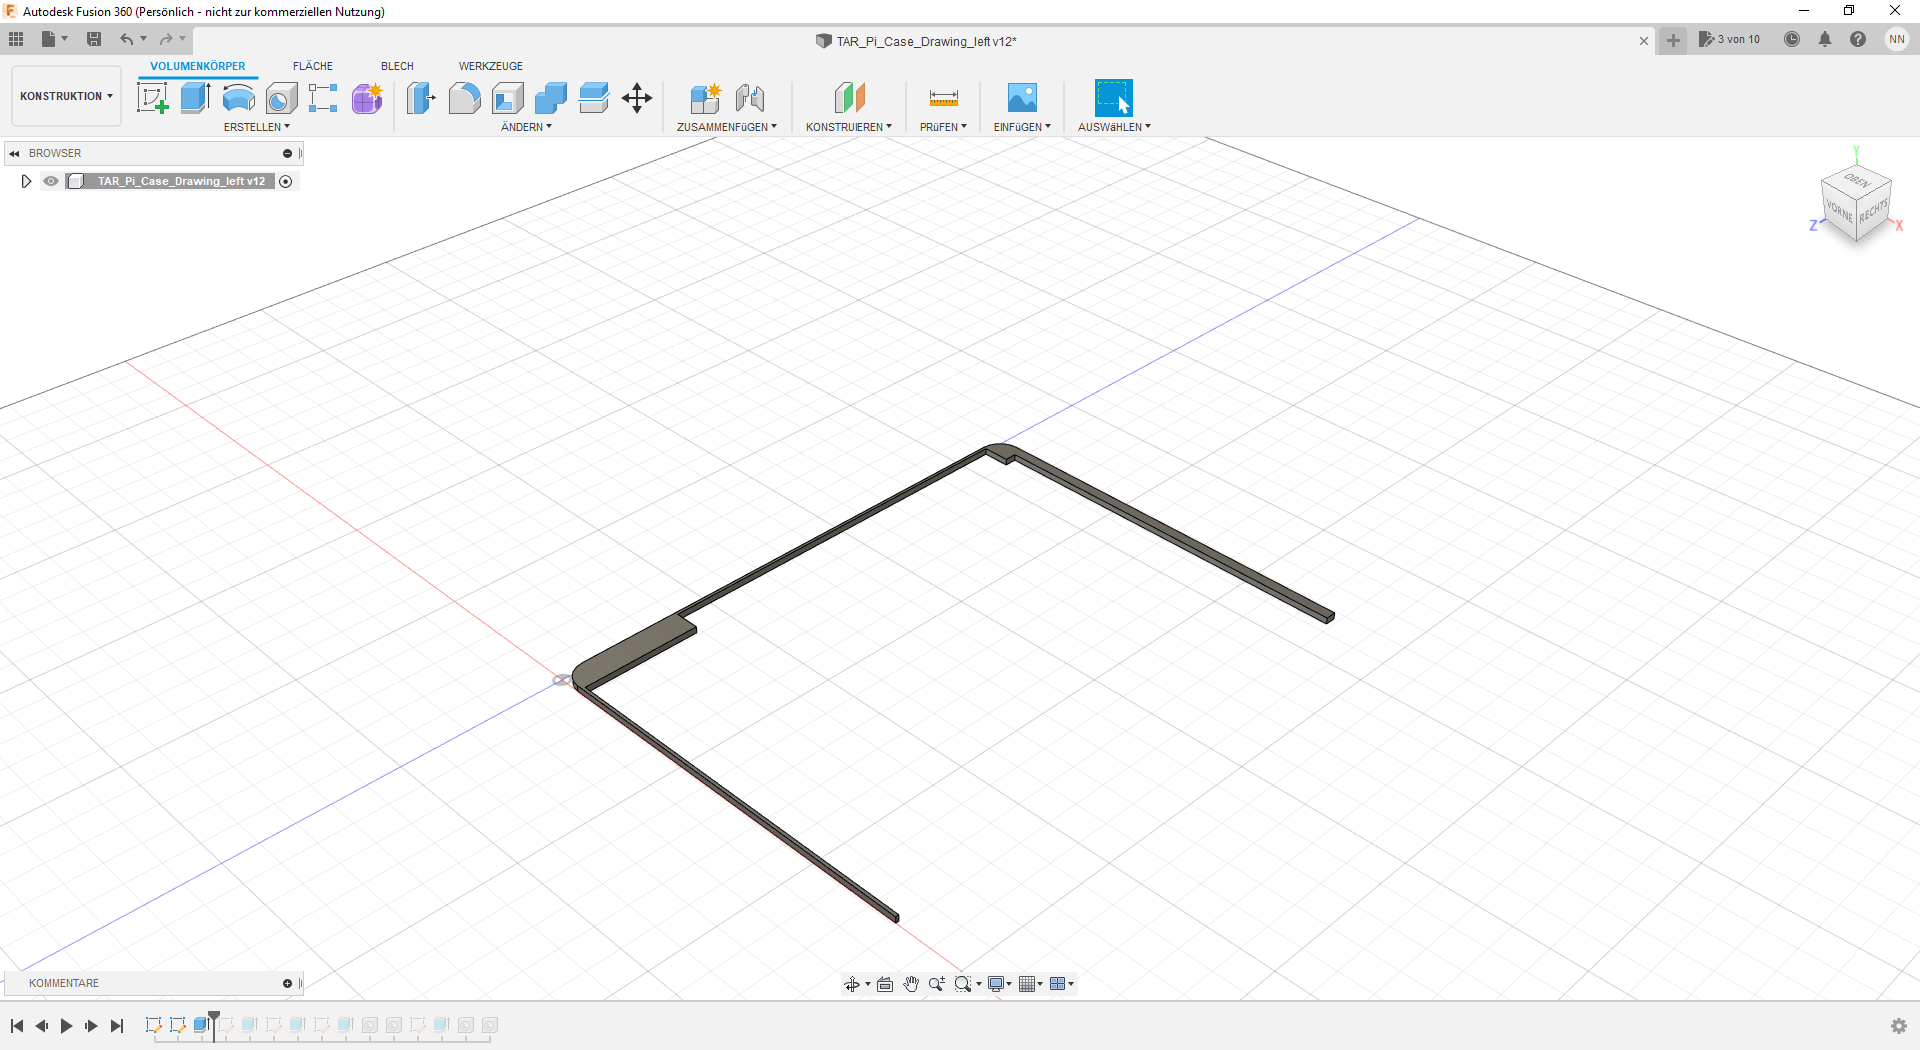
\includegraphics[width=\linewidth]{img/konstruktion_gehaeuse_links_001.png}
		\caption[Extrusion der Grundzeichnung]{Extrusion der Grundzeichnung}
		\label{fig:design-left-01}
	\end{subfigure}
	\begin{subfigure}[t]{.3\linewidth}
		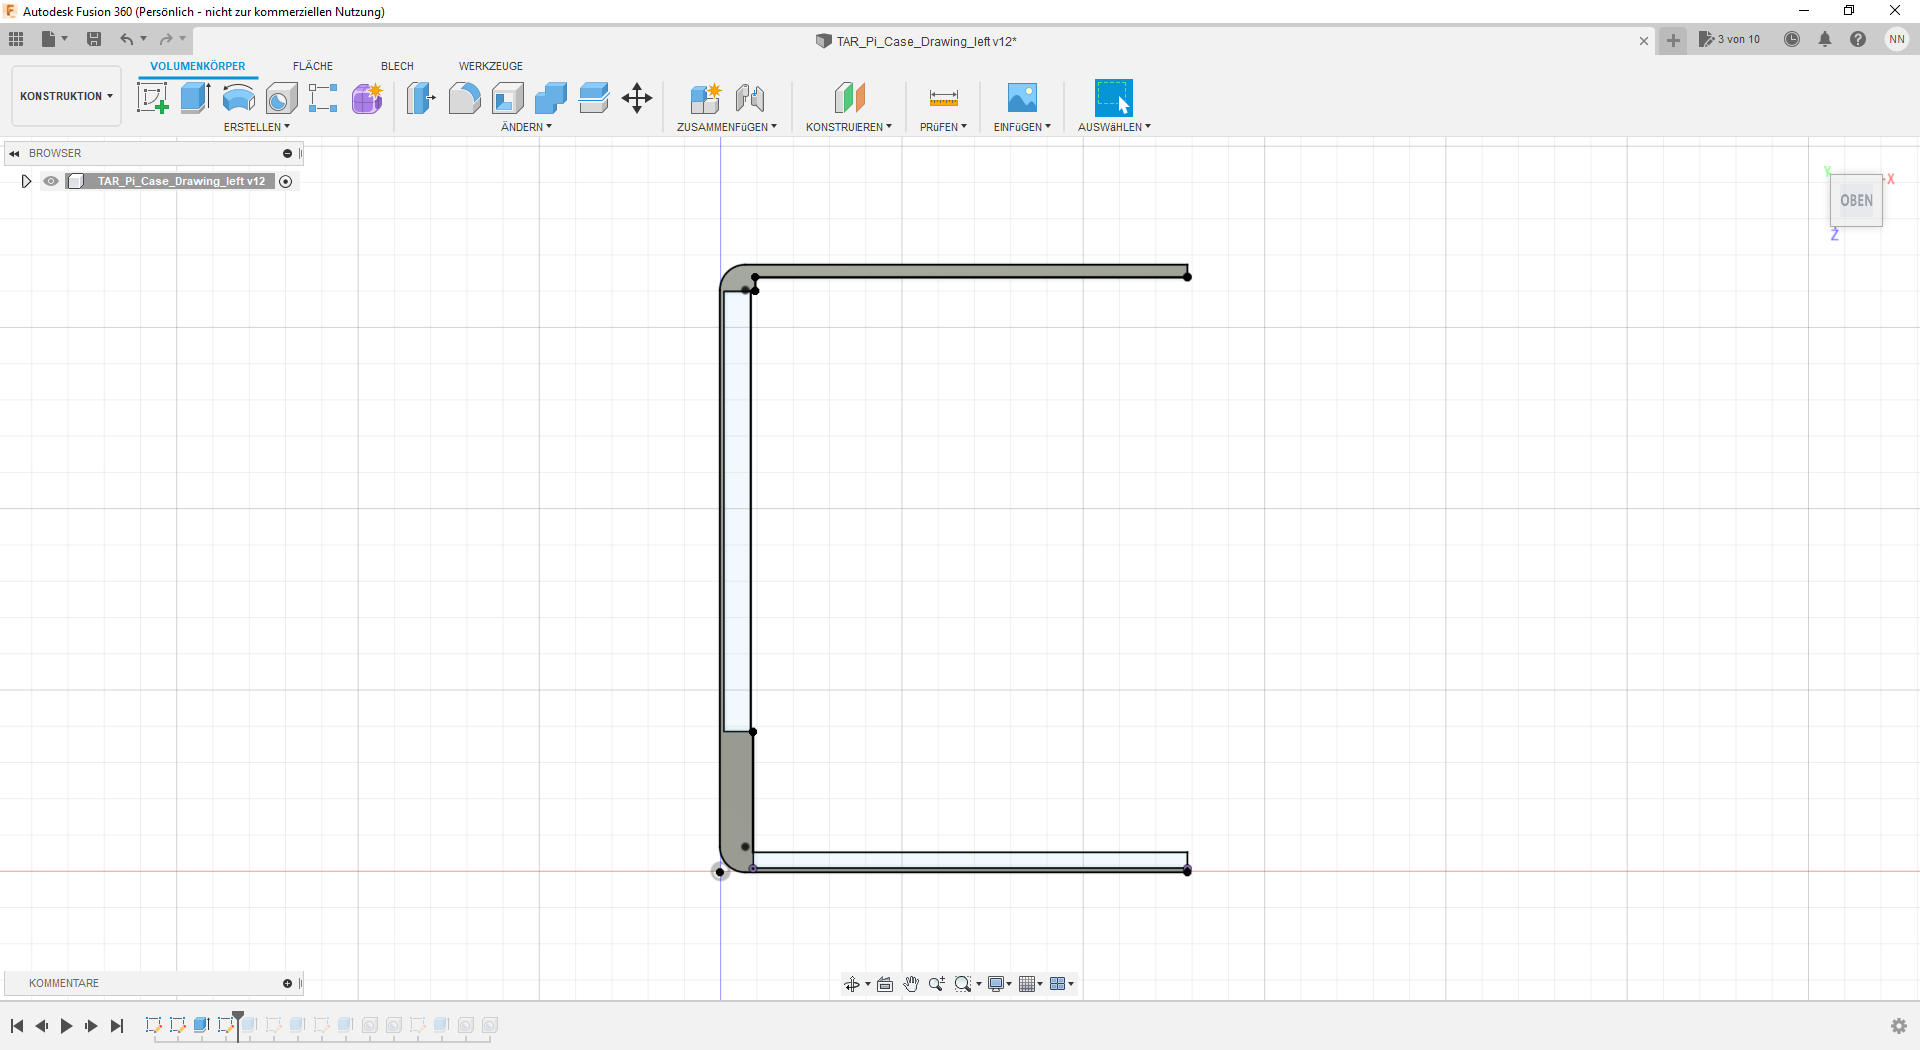
\includegraphics[width=\linewidth]{img/konstruktion_gehaeuse_links_002.png}
		\caption[Erstellung der Folgezeichnung um Blech]{Erstellung der Folgezeichnung um Blech}
		\label{fig:design-left-02}
	\end{subfigure}
	\begin{subfigure}[t]{.3\linewidth}
		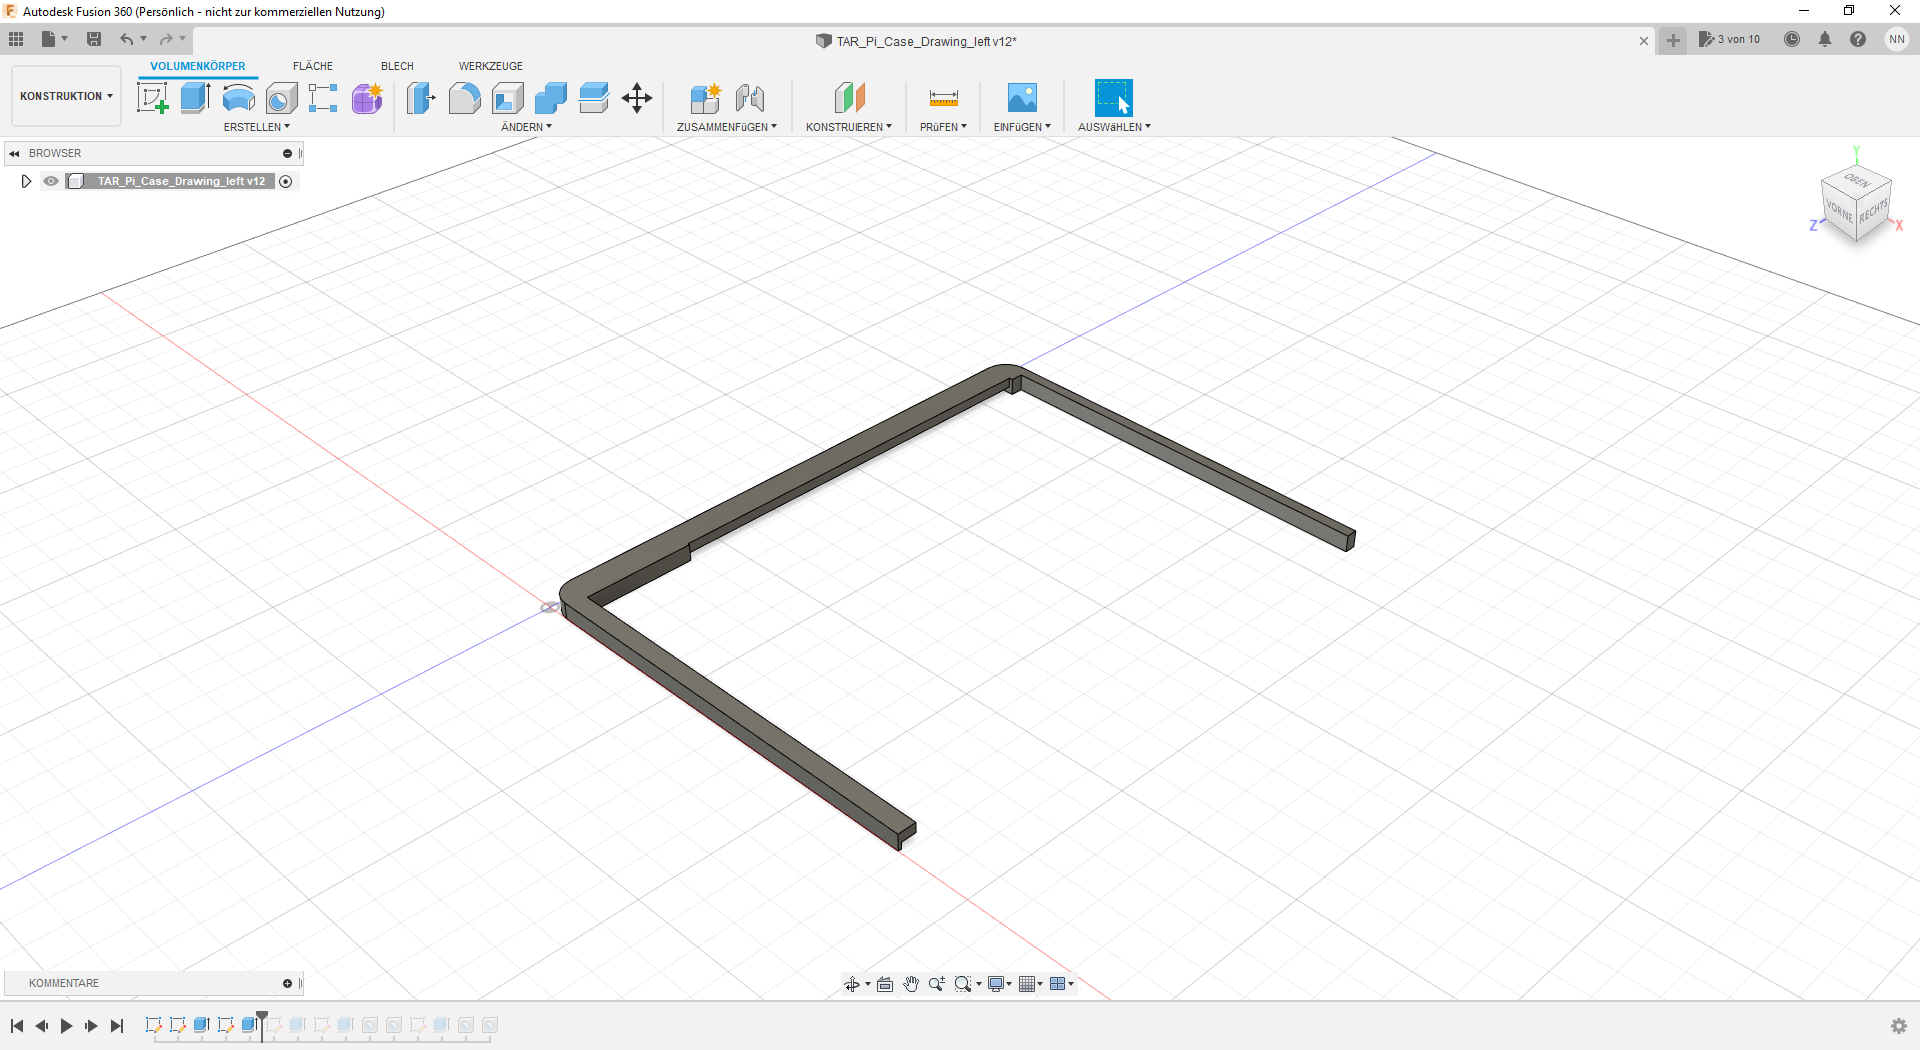
\includegraphics[width=\linewidth]{img/konstruktion_gehaeuse_links_003.png}
		\caption[Extrusion der neuen Zeichnung]{Extrusion der neuen Zeichnung}
		\label{fig:design-left-03}
	\end{subfigure}
	\begin{subfigure}[t]{.3\linewidth}
		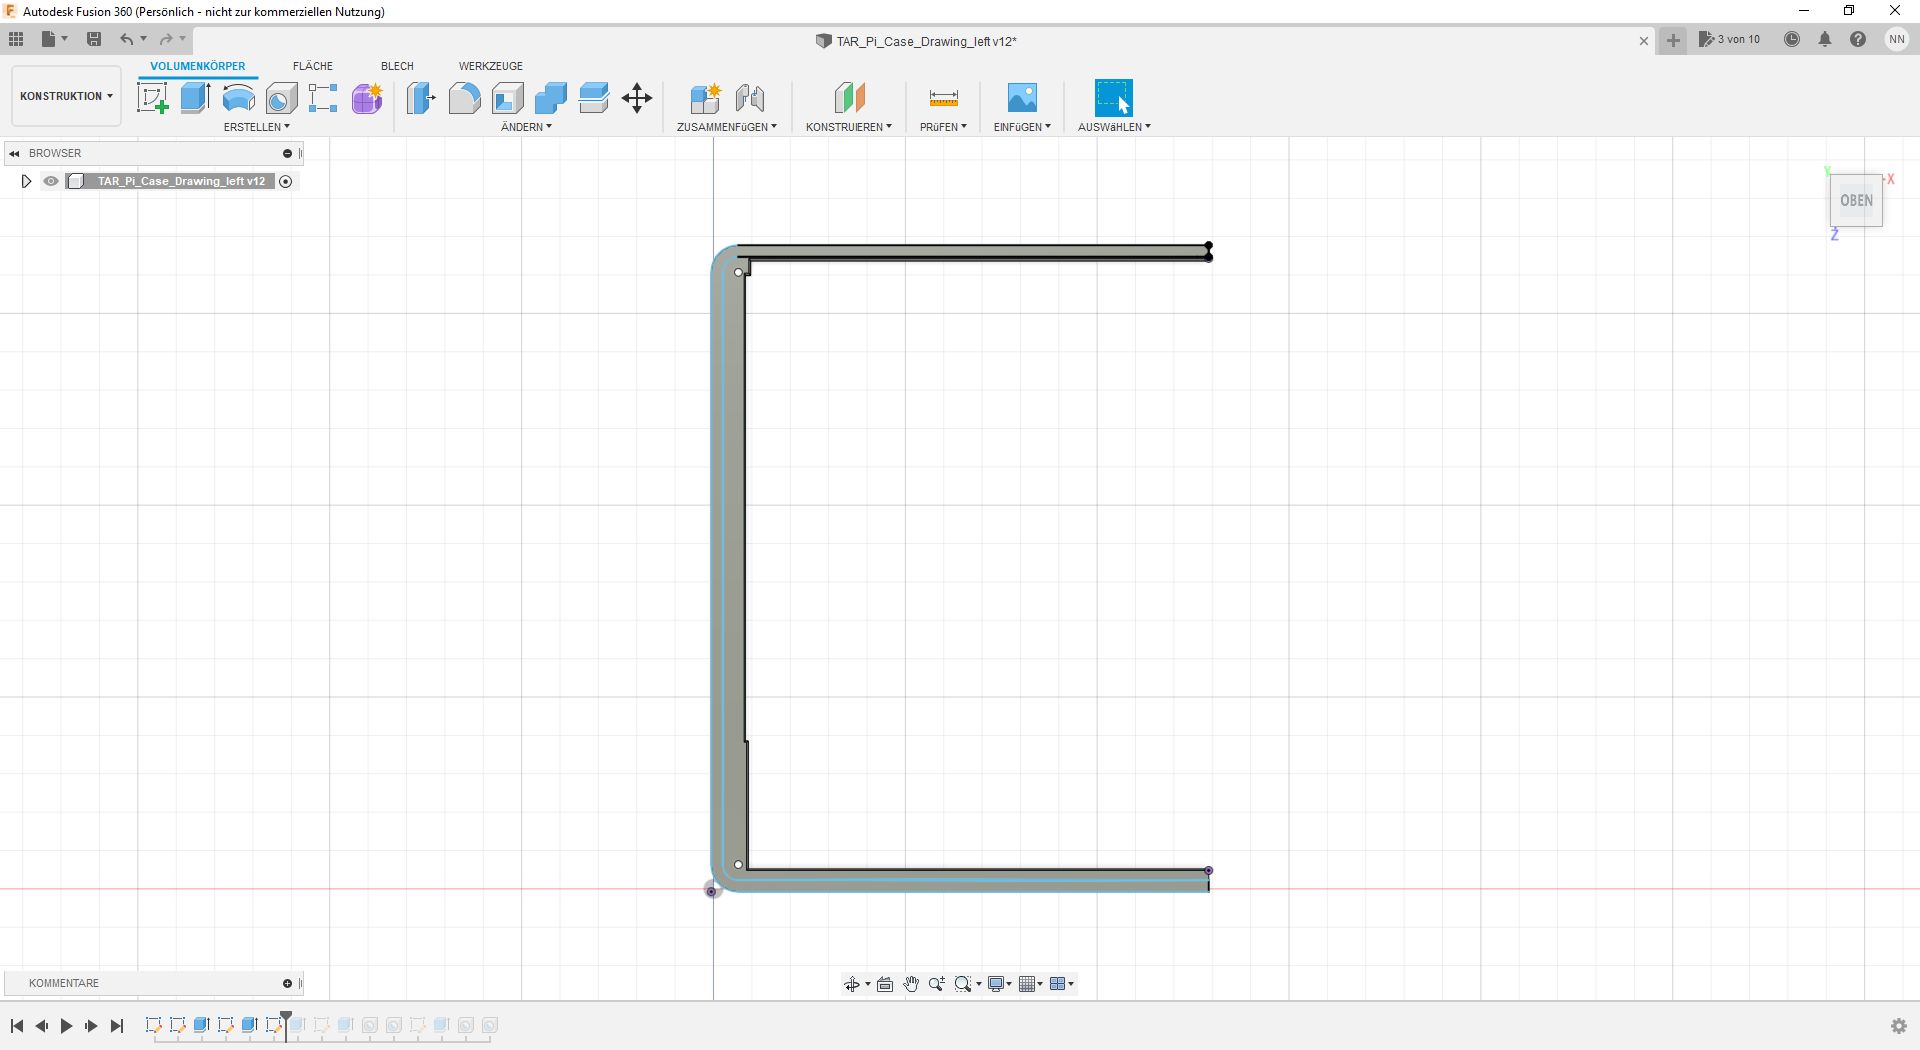
\includegraphics[width=\linewidth]{img/konstruktion_gehaeuse_links_004.png}
		\caption[Zeichnung der Hauptwandstärke]{Zeichnung der Hauptwandstärke}
		\label{fig:design-left-04}
	\end{subfigure}
	\begin{subfigure}[t]{.3\linewidth}
		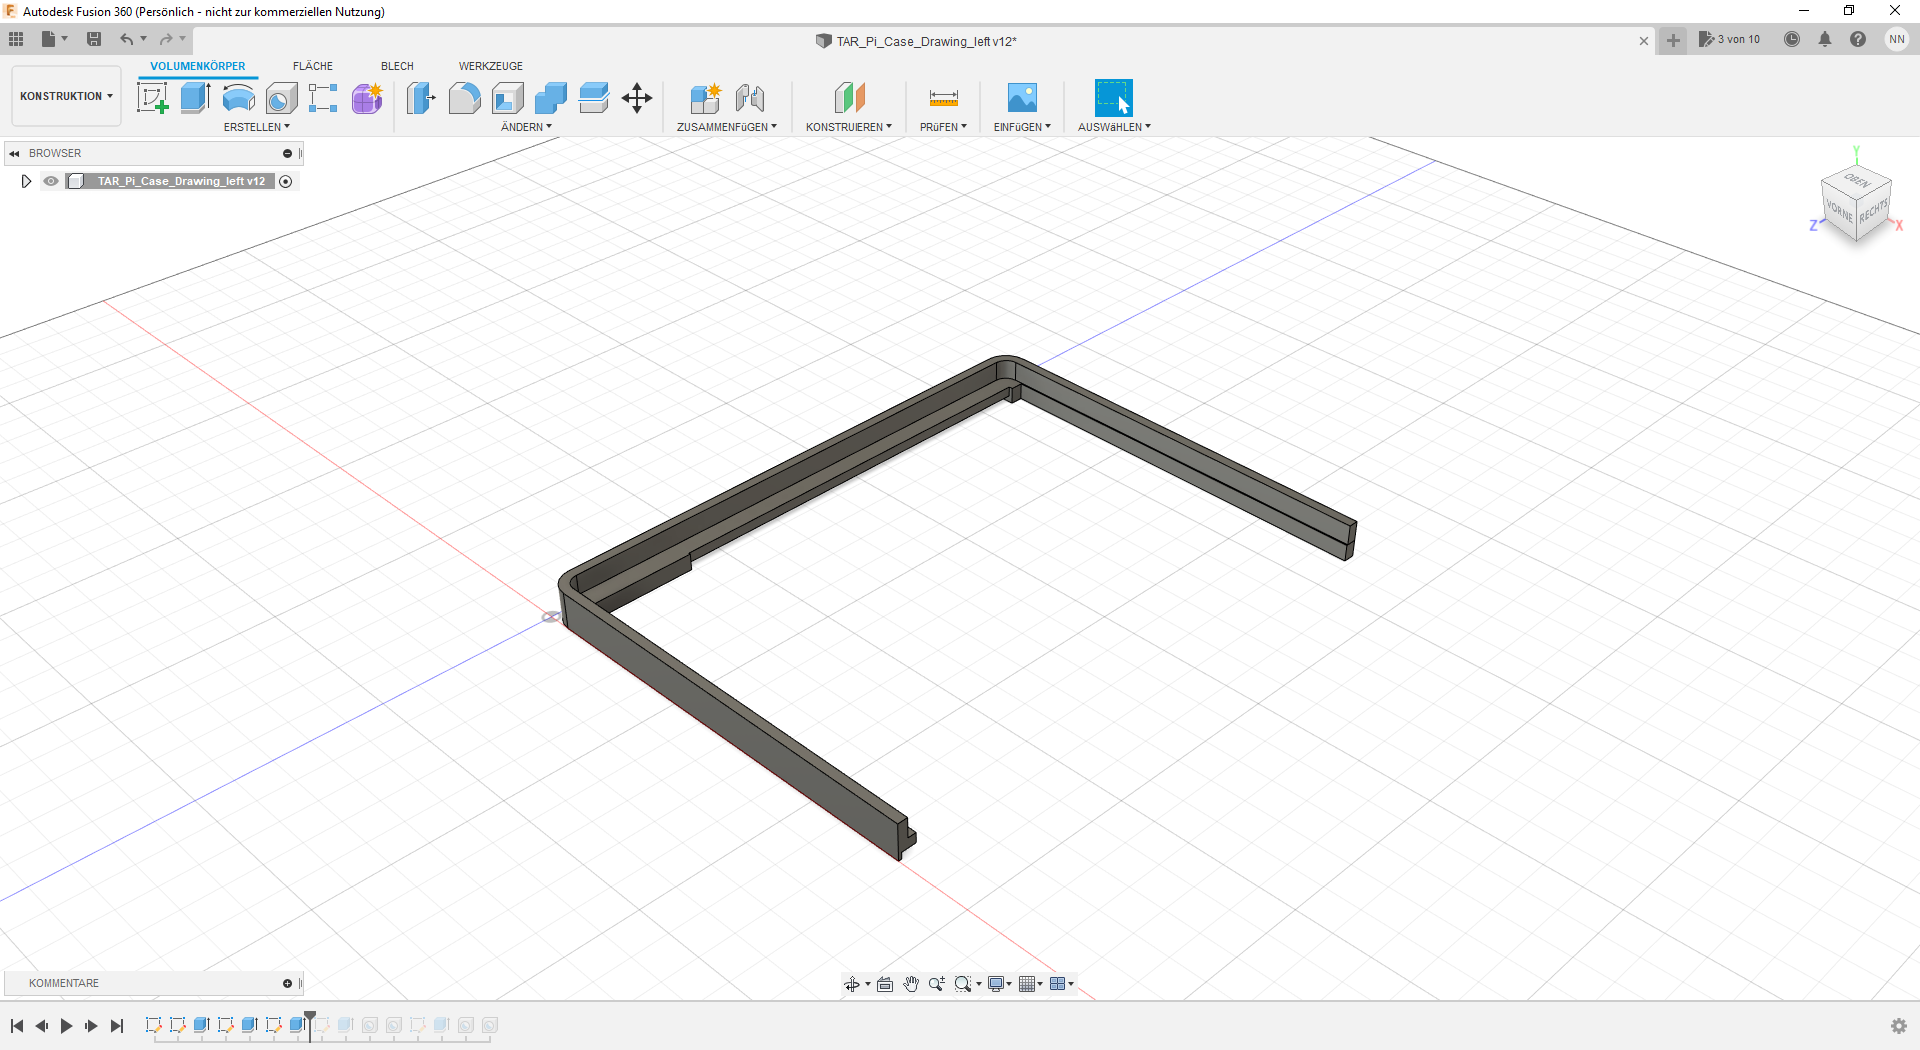
\includegraphics[width=\linewidth]{img/konstruktion_gehaeuse_links_005.png}
		\caption[Extrusion der Hauptwand]{Extrusion der Hauptwand}
		\label{fig:design-left-05}
	\end{subfigure}
	\begin{subfigure}[t]{.3\linewidth}
		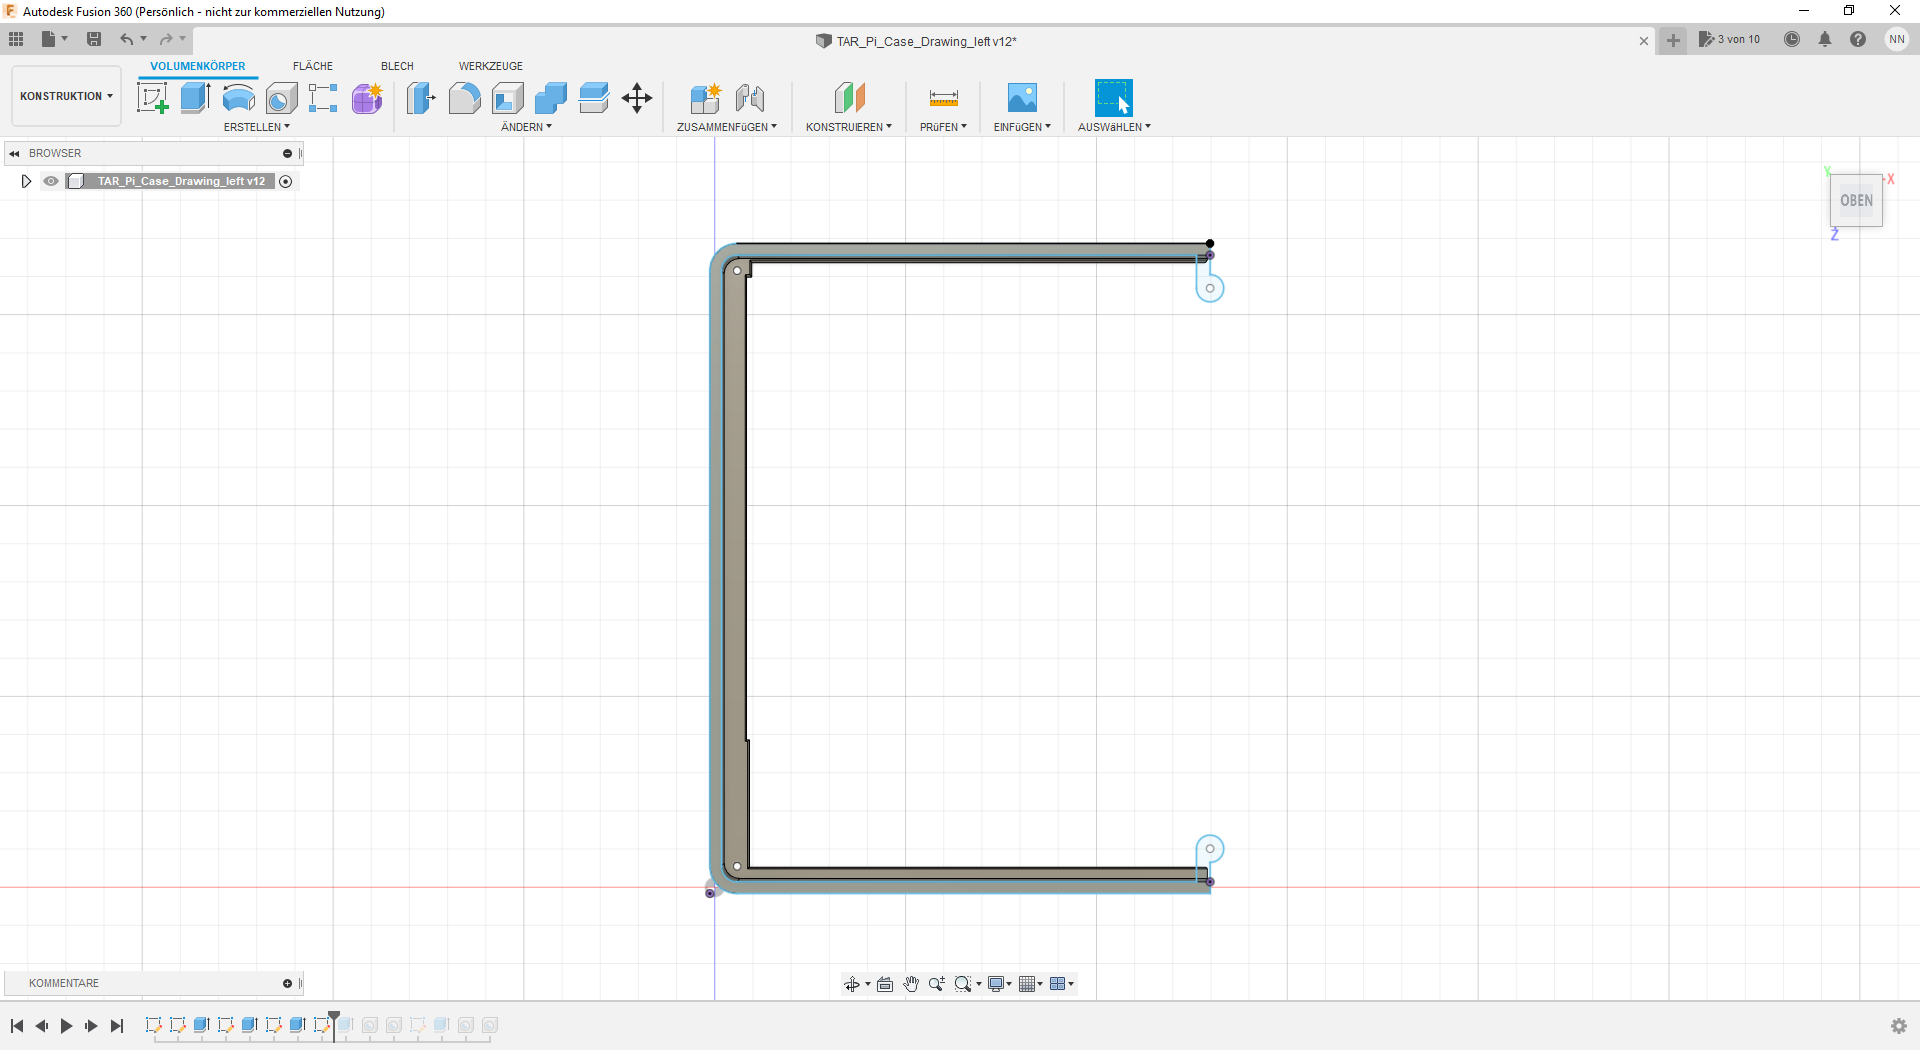
\includegraphics[width=\linewidth]{img/konstruktion_gehaeuse_links_006.png}
		\caption[Zeichnung der Verbindungsstücke]{Zeichnung der Verbindungsstücke}
		\label{fig:design-left-06}
	\end{subfigure}
	\begin{subfigure}[t]{.3\linewidth}
		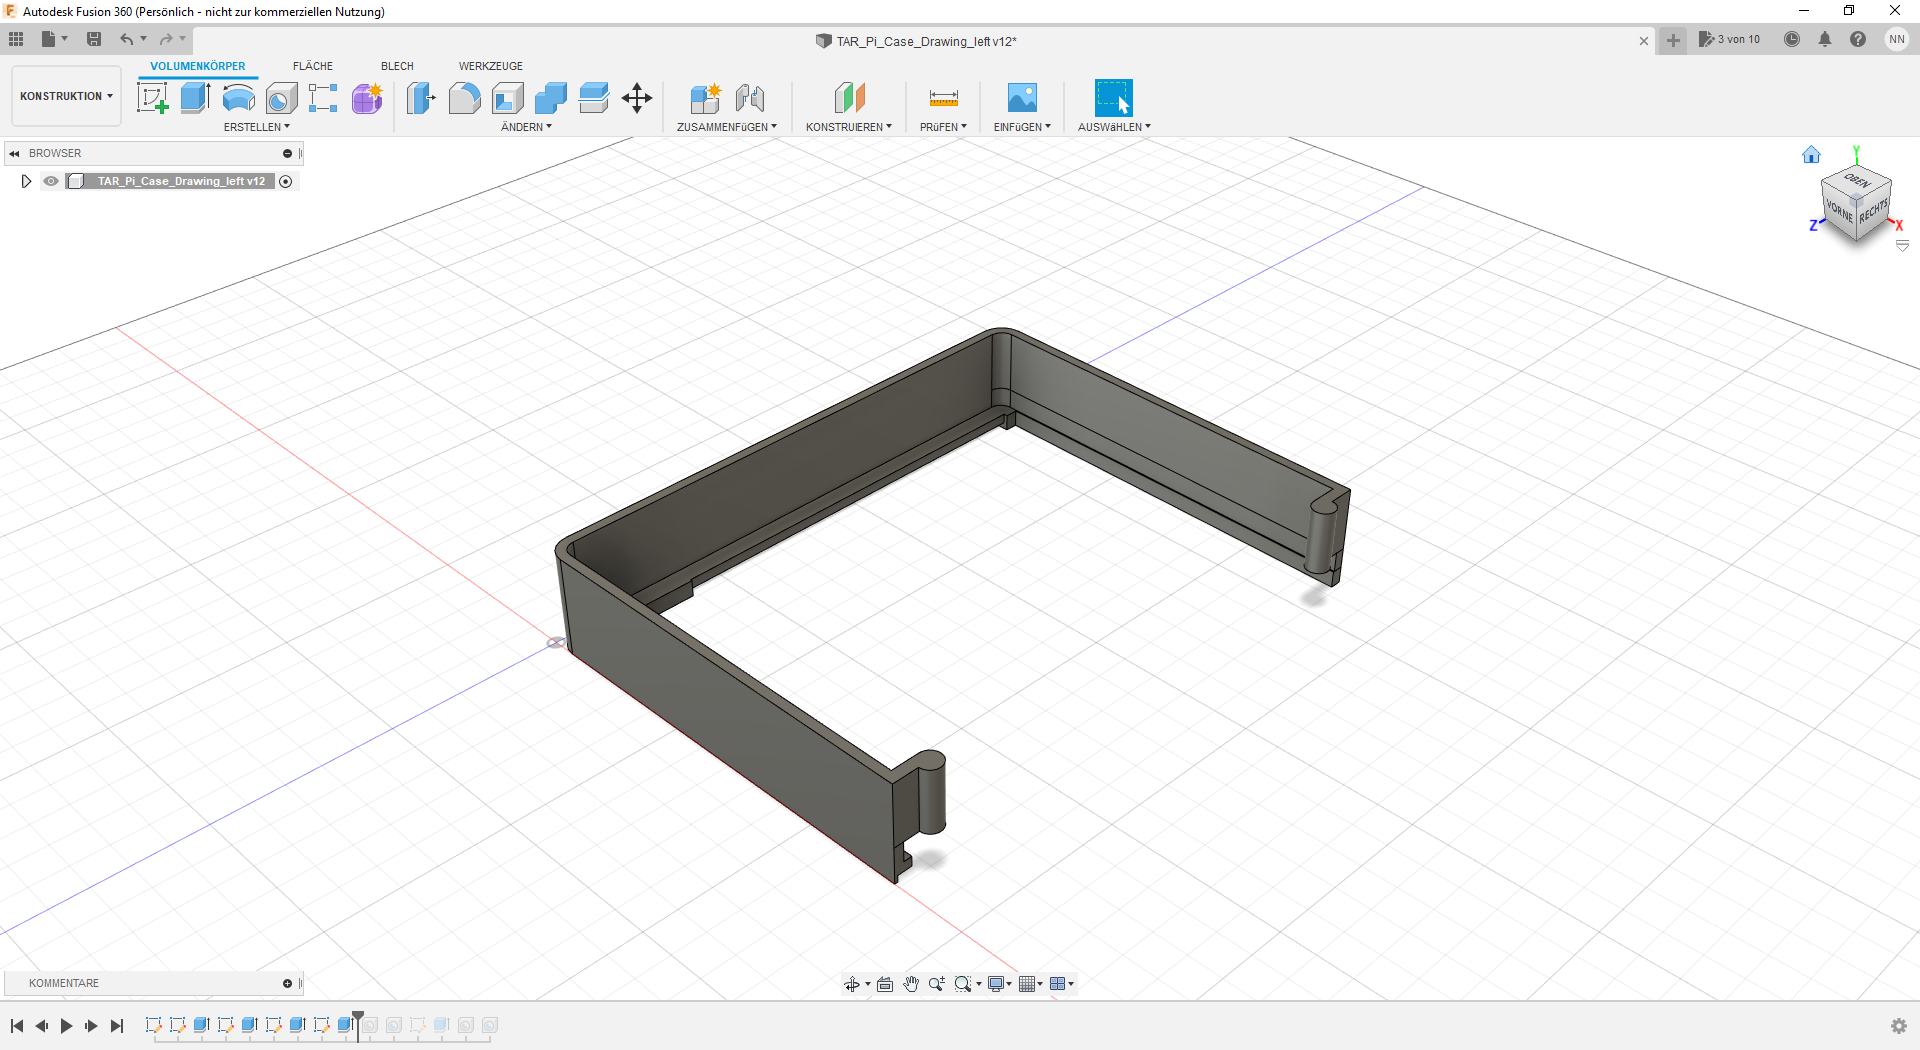
\includegraphics[width=\linewidth]{img/konstruktion_gehaeuse_links_007.png}
		\caption[Extrusion der Hauptwand mit Verbindungsstücken]{Extrusion der Hauptwand mit Verbindungsstücken}
		\label{fig:design-left-07}
	\end{subfigure}
	\begin{subfigure}[t]{.3\linewidth}
		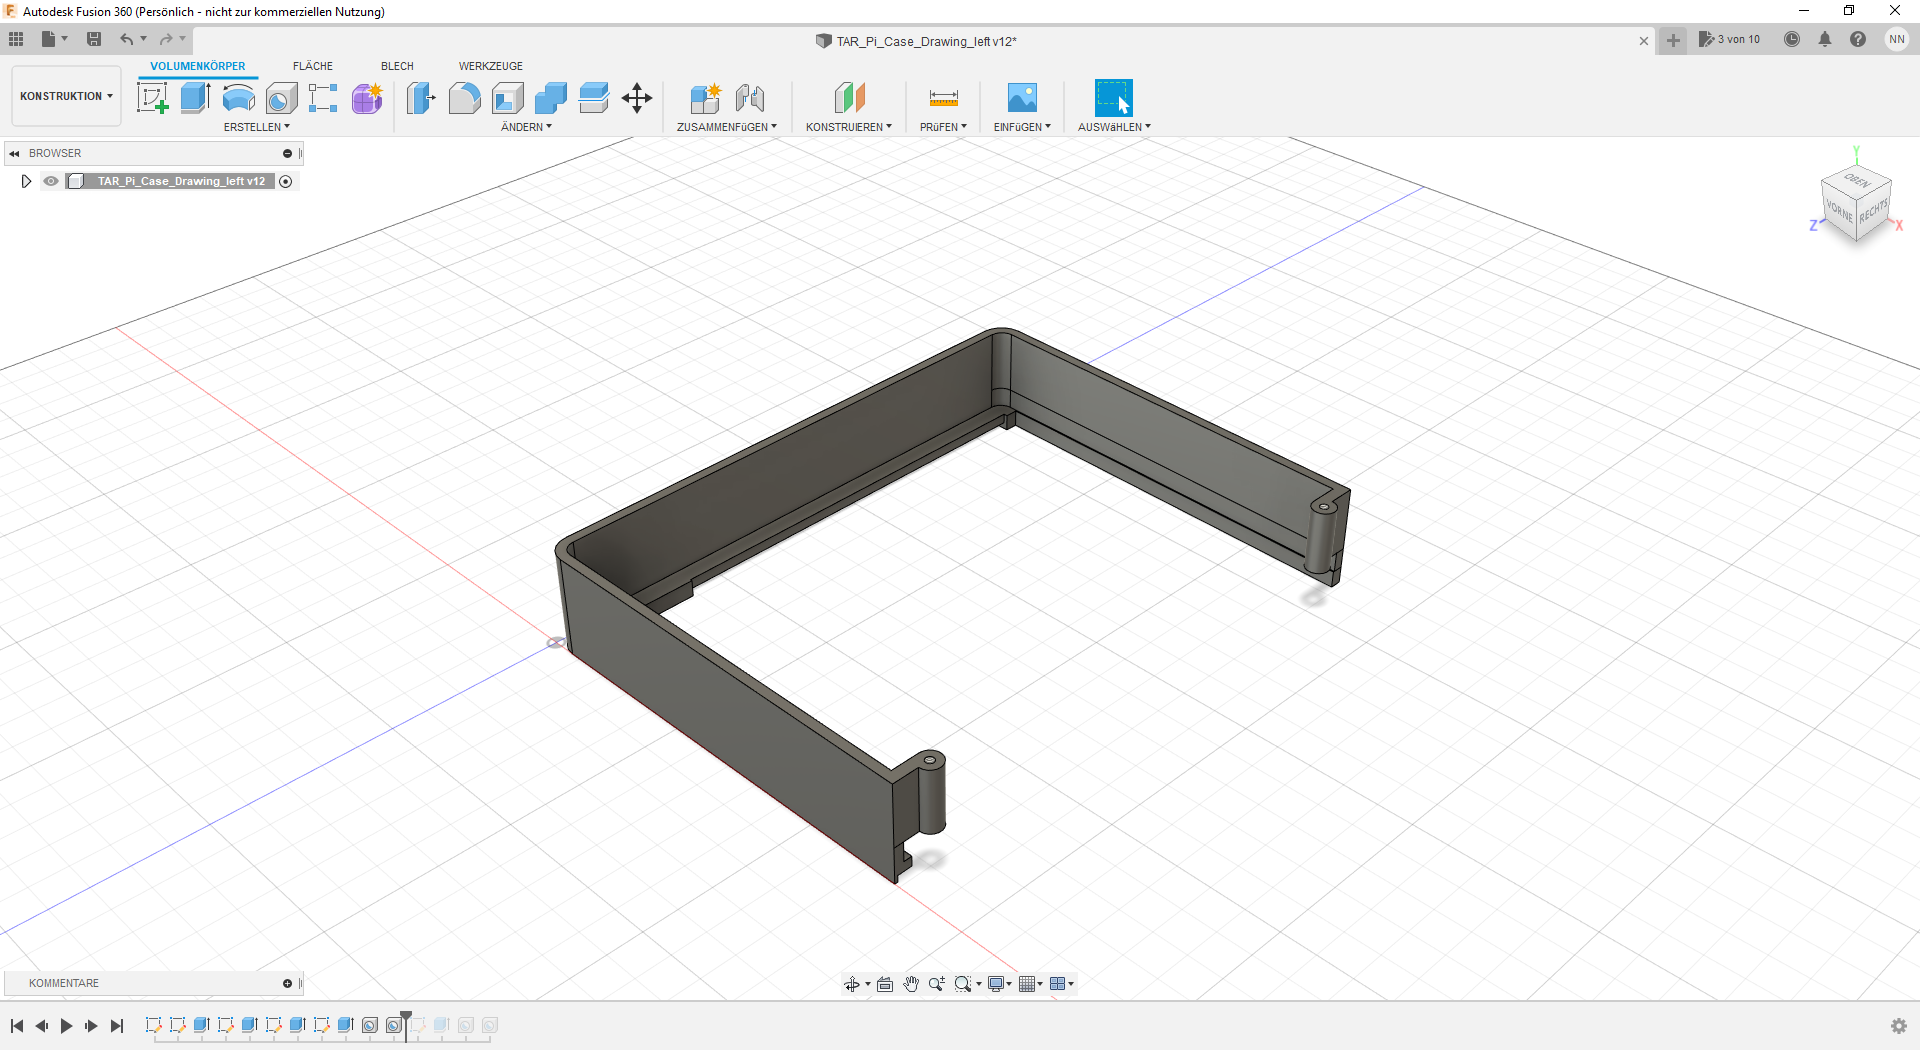
\includegraphics[width=\linewidth]{img/konstruktion_gehaeuse_links_008.png}
		\caption[Bohrung für Schrauben]{Bohrung für Schrauben}
		\label{fig:design-left-08}
	\end{subfigure}
	\begin{subfigure}[t]{.3\linewidth}
		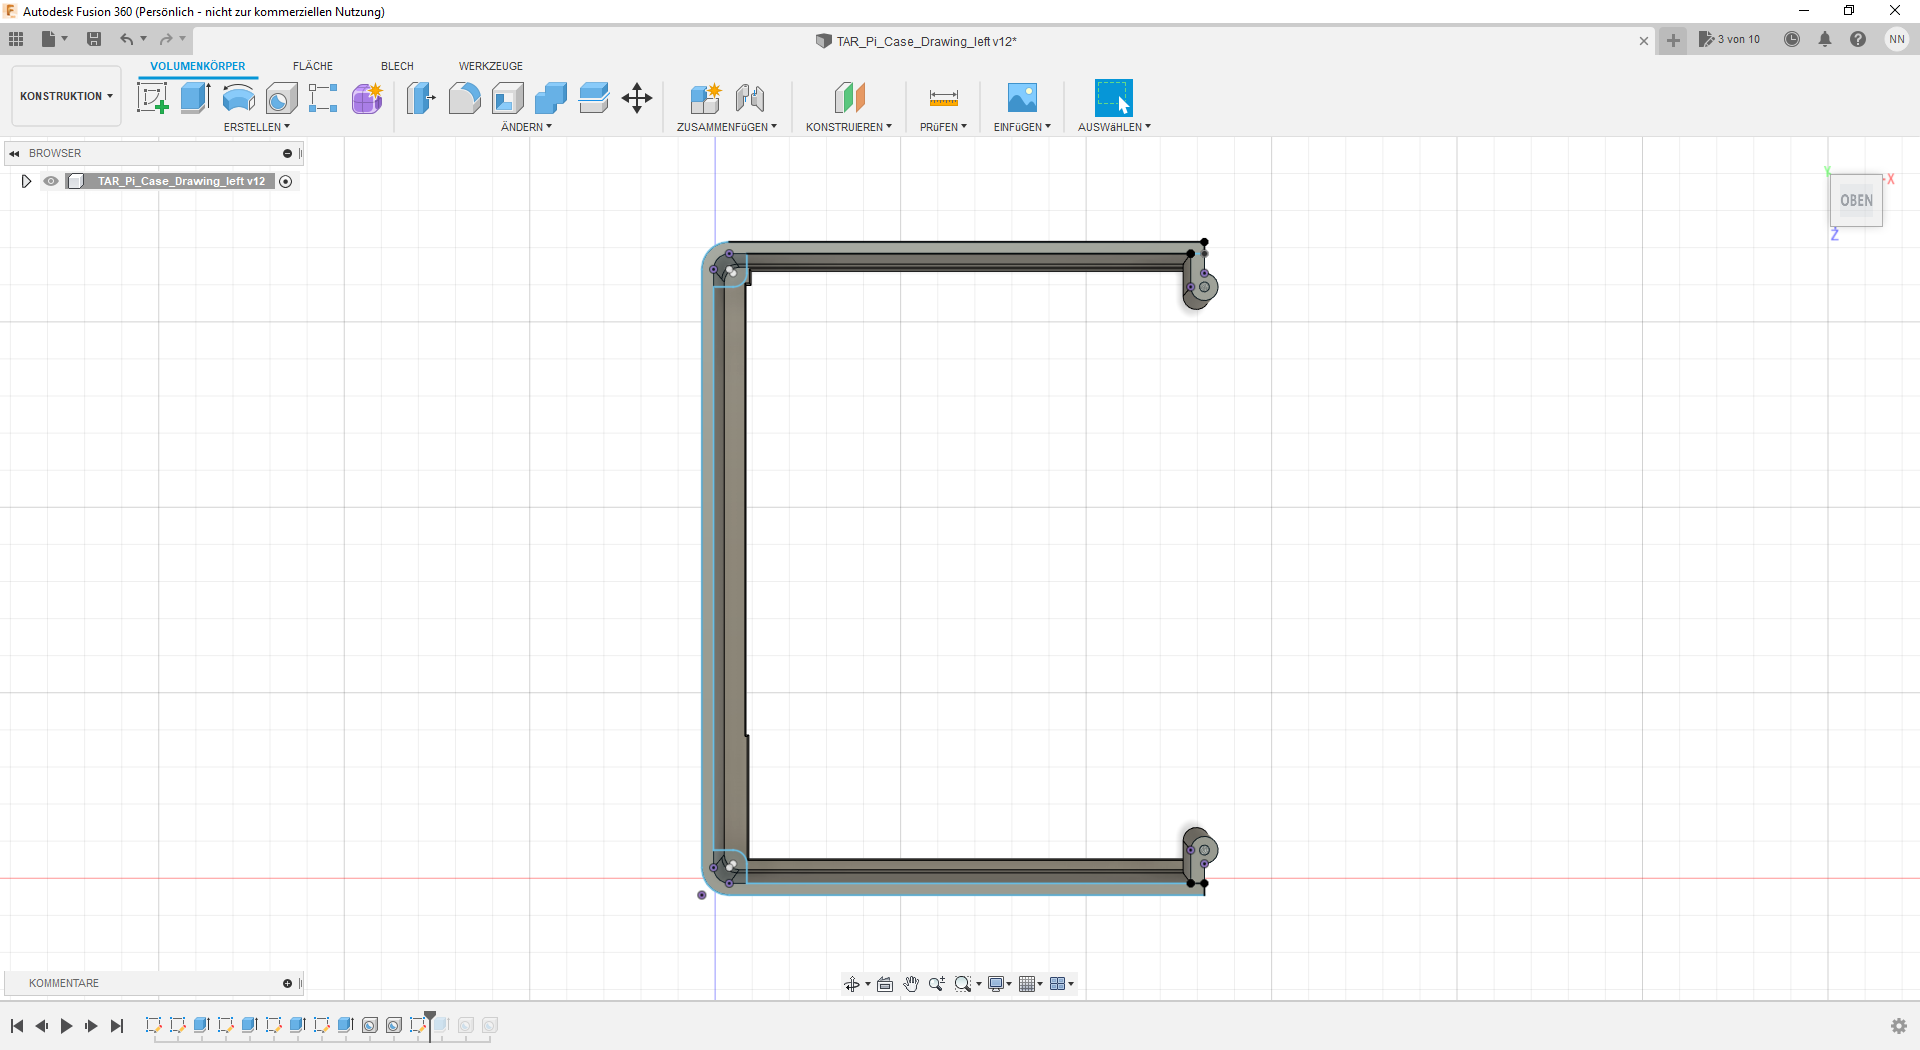
\includegraphics[width=\linewidth]{img/konstruktion_gehaeuse_links_009.png}
		\caption[Zeichnung der Deckelverbindung]{Zeichnung der Deckelverbindung}
		\label{fig:design-left-09}
	\end{subfigure}
	\begin{subfigure}[t]{.3\linewidth}
		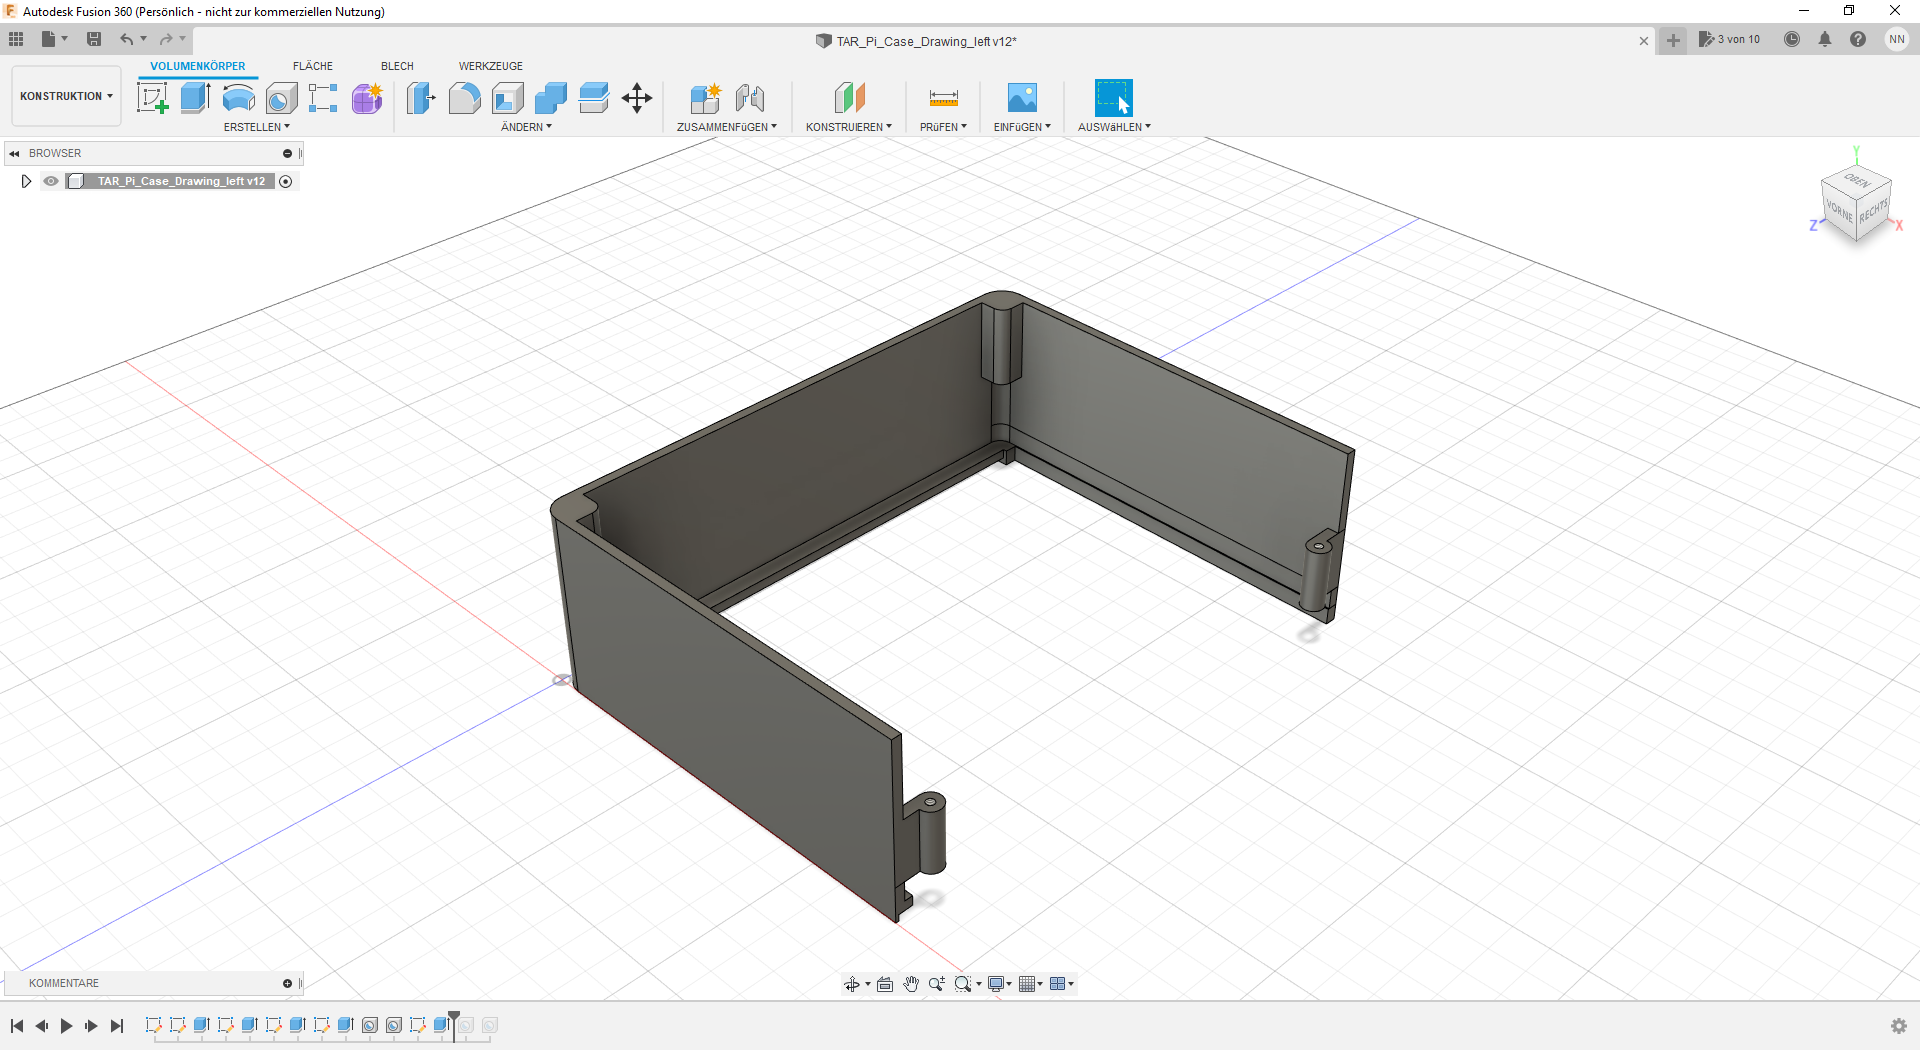
\includegraphics[width=\linewidth]{img/konstruktion_gehaeuse_links_010.png}
		\caption[Extrusion der Hauptwand mit Deckelverbindung]{Extrusion der Hauptwand mit Deckelverbindung}
		\label{fig:design-left-10}
	\end{subfigure}
	\begin{subfigure}[t]{.3\linewidth}
		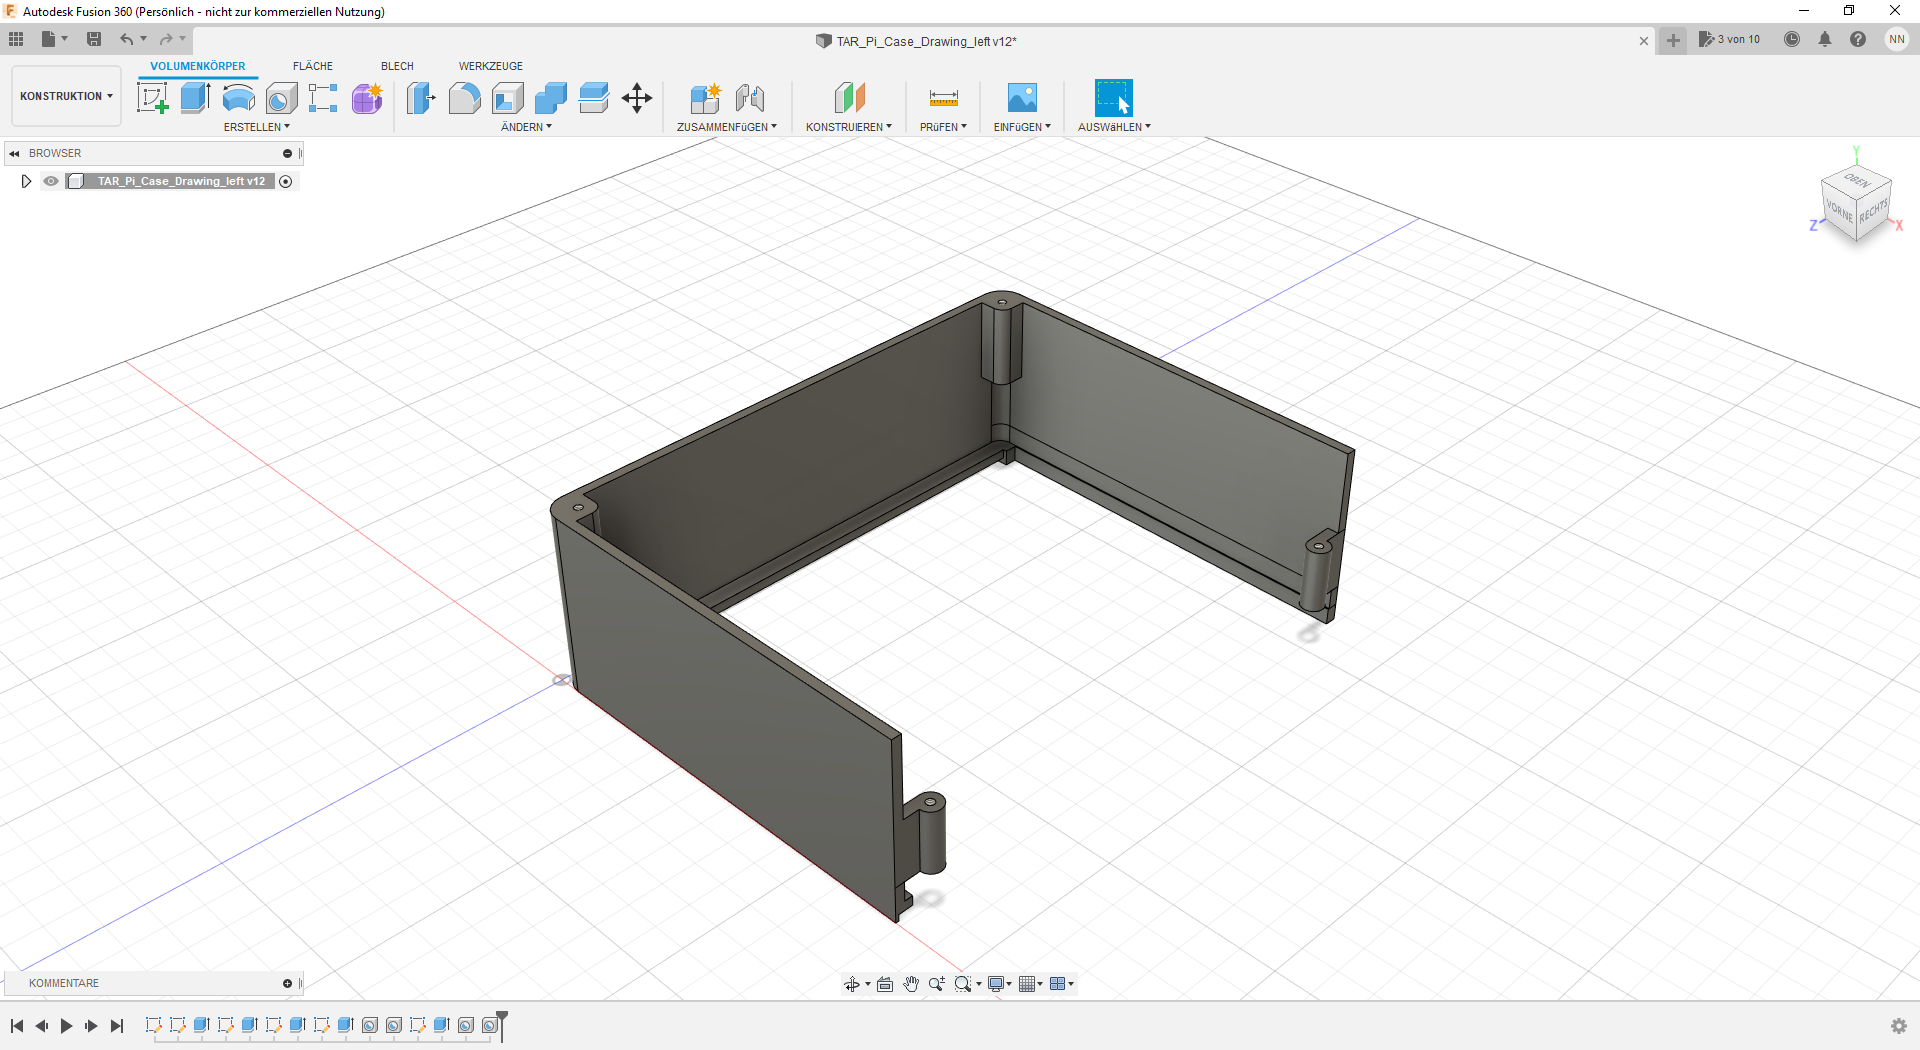
\includegraphics[width=\linewidth]{img/konstruktion_gehaeuse_links_011.png}
		\caption[Bohrungen der Deckelverbindung]{Bohrungen der Deckelverbindung}
		\label{fig:design-left-11}
	\end{subfigure}
	\caption[Entwurf des linken Wandteils]{Entwurf des linken Wandteils}
	\label{fig:design-left}
\end{figure}\par
\paragraph{Rechtes Wandteil}
Beim rechten Teil des Gehäuses war die Vorgehensweise weitestgehend die selbe wie beim linken Gehäuseteil (vgl. \ref{fig:design-right-01} - \ref{fig:design-right-08} mit \ref{fig:design-left}). Der Unterschied zwischen beiden Teilen, abgesehen von den Verbindungsstücken und der Aussparung für das Flachkabel des Bildschirms, waren die Aussparungen für Lüfter, Antenne, Netzwerkanschluss und Strombuchse. Für den Lüfter und die Antenne wurde auf der ,,Oberseite'' des Gehäuses eine Zeichnung aufgelegt (vgl. \ref{fig:design-right-09}), die dann ins Negative extruiert wurde, was die gezeichnete Fläche aus dem Körper löscht (vgl. \ref{fig:design-right-10}). Auf ähnliche Weise wurde die Aussparung für eine RJ45-Verlängerung und eine 5,5 mm DC-Buchse gesetzt. Zuerst wurde die Zeichnung für die Aussparung auf die Seite gelegt (vgl. \ref{fig:design-right-11}), die dann ebenfalls ins Negative extruiert wurde (vgl. \ref{fig:design-right-12}). Um für die Befestigung der 5,5 mm DC-Buchse eine Unterlage im Gehäuse zu haben, wurde der Grundriss eines Rechtecks auf die Innenseite des Gehäusebodens gelegt (vgl. \ref{fig:design-right-13}) und extruiert (vgl. \ref{fig:design-right-14}), um die Möglichkeit zu bieten, die Buchse im Gehäuse zu verkleben. Damit die Buchse nicht zu tief im Gehäuse steckt, wurde eine Zeichnung eines konzentrischen Kreises auf die bereits vorhandene Aussparung auf die Innenseite gelegt  (vgl. \ref{fig:design-right-15}) und dann um einige Millimeter ins Negative extruiert, um die Aussparung zu generieren (vgl. \ref{fig:design-right}).\\
\begin{figure}[h!tb]
	\begin{subfigure}[t]{.3\linewidth}
		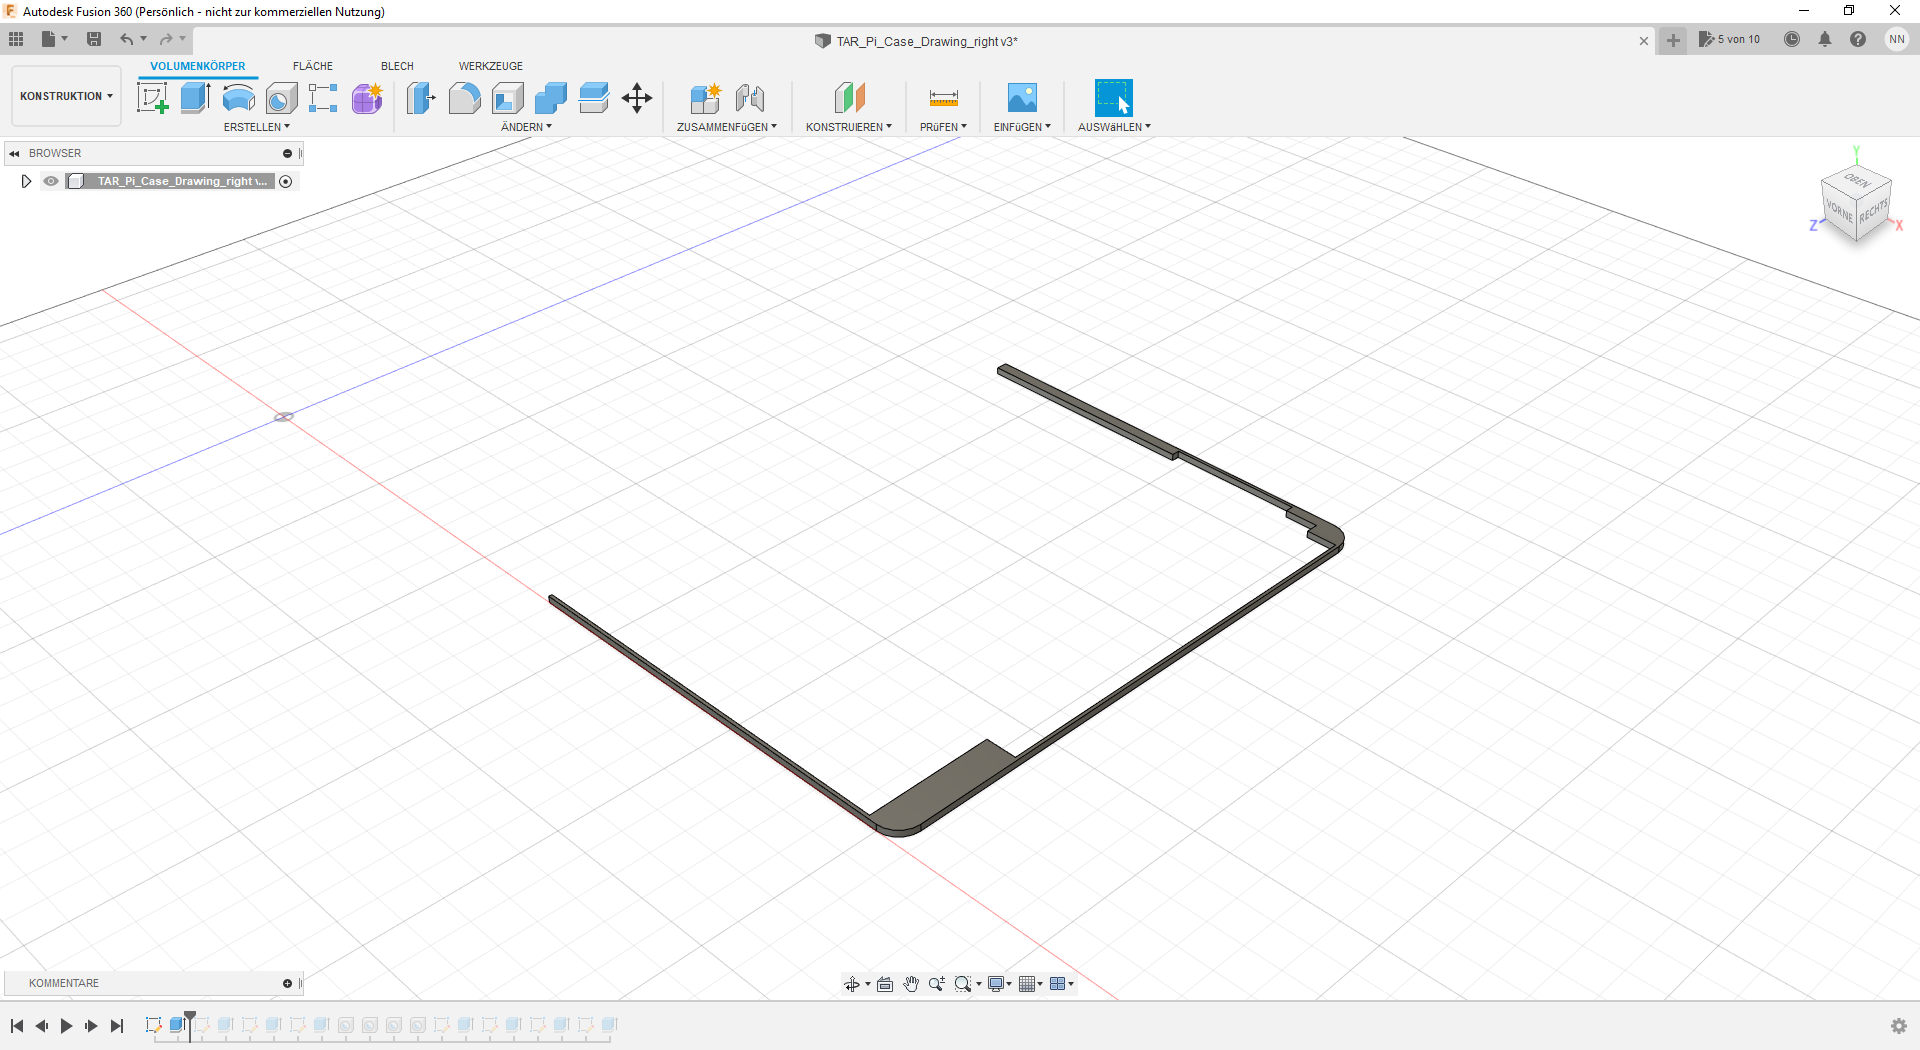
\includegraphics[width=\linewidth]{img/konstruktion_gehaeuse_rechts_001.png}
		\caption[]{}
		\label{fig:design-right-01}
	\end{subfigure}
	\begin{subfigure}[t]{.3\linewidth}
		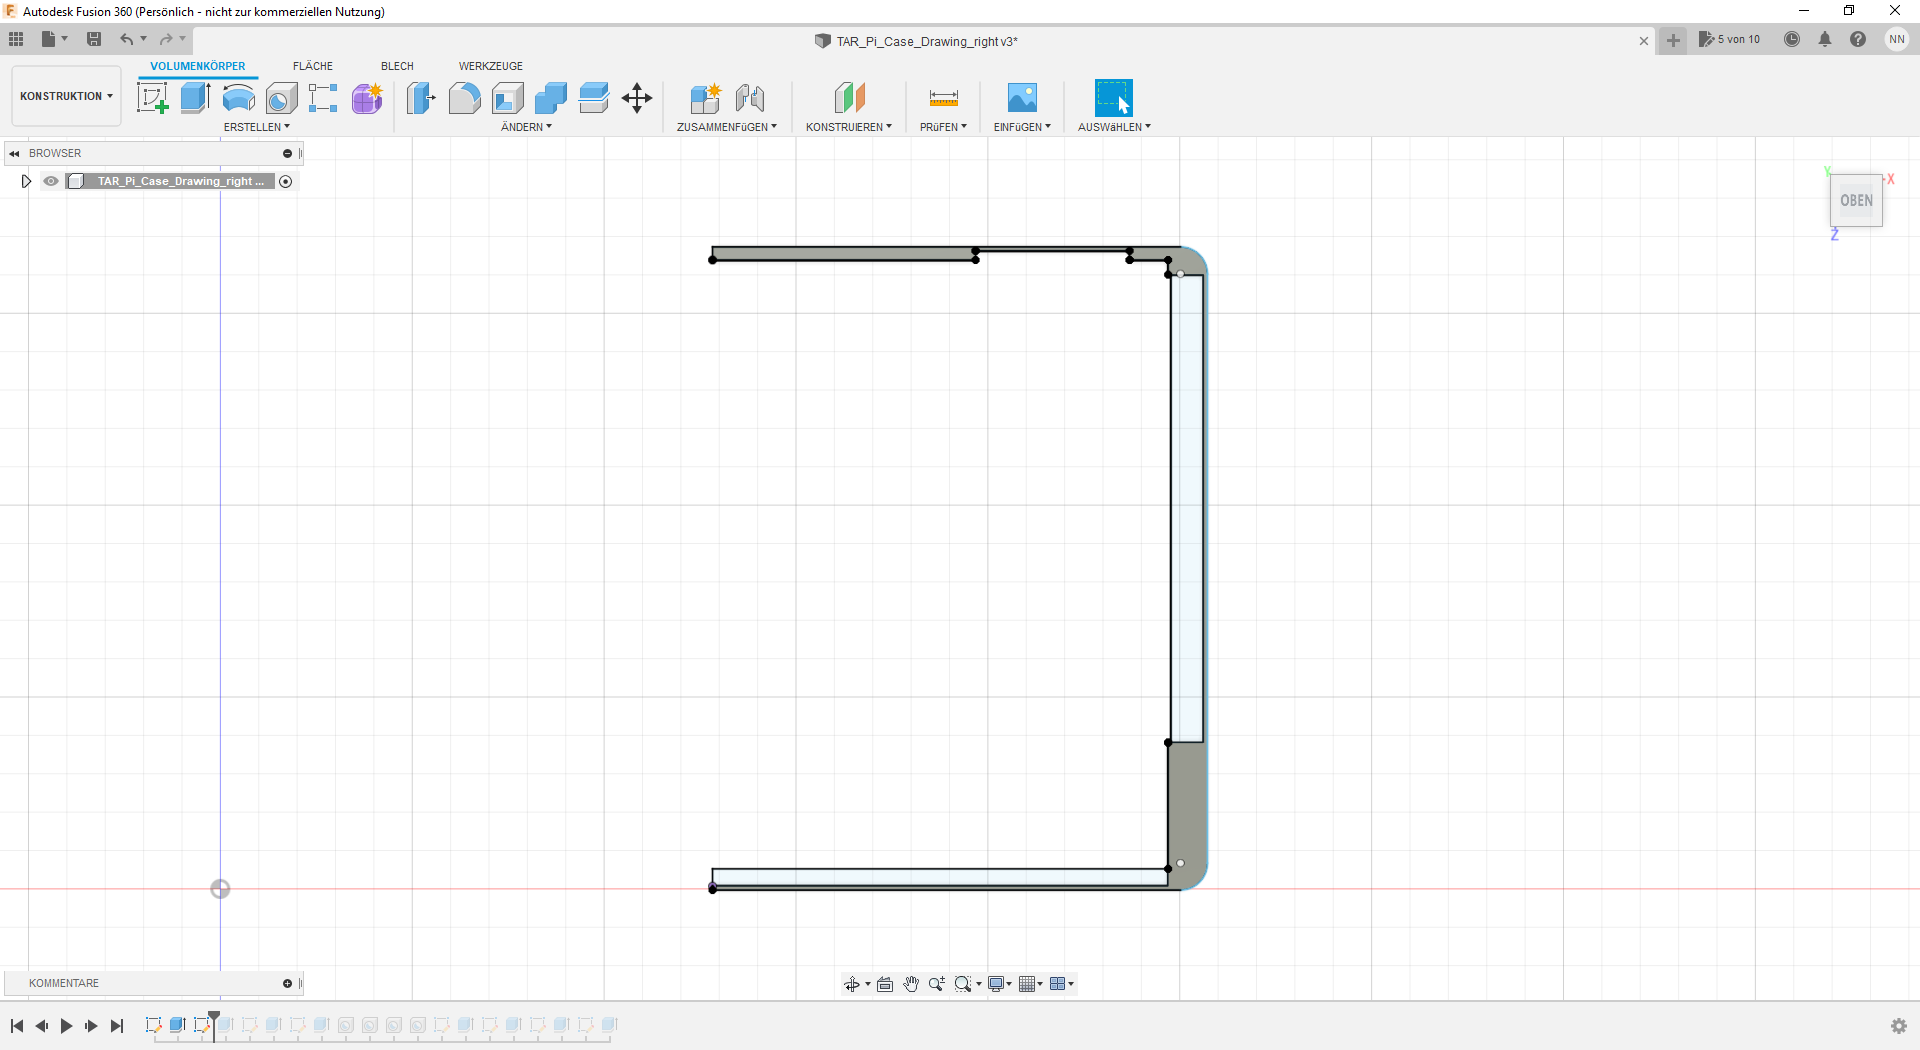
\includegraphics[width=\linewidth]{img/konstruktion_gehaeuse_rechts_002.png}
		\caption[]{}
		\label{fig:design-right-02}
	\end{subfigure}
	\begin{subfigure}[t]{.3\linewidth}
		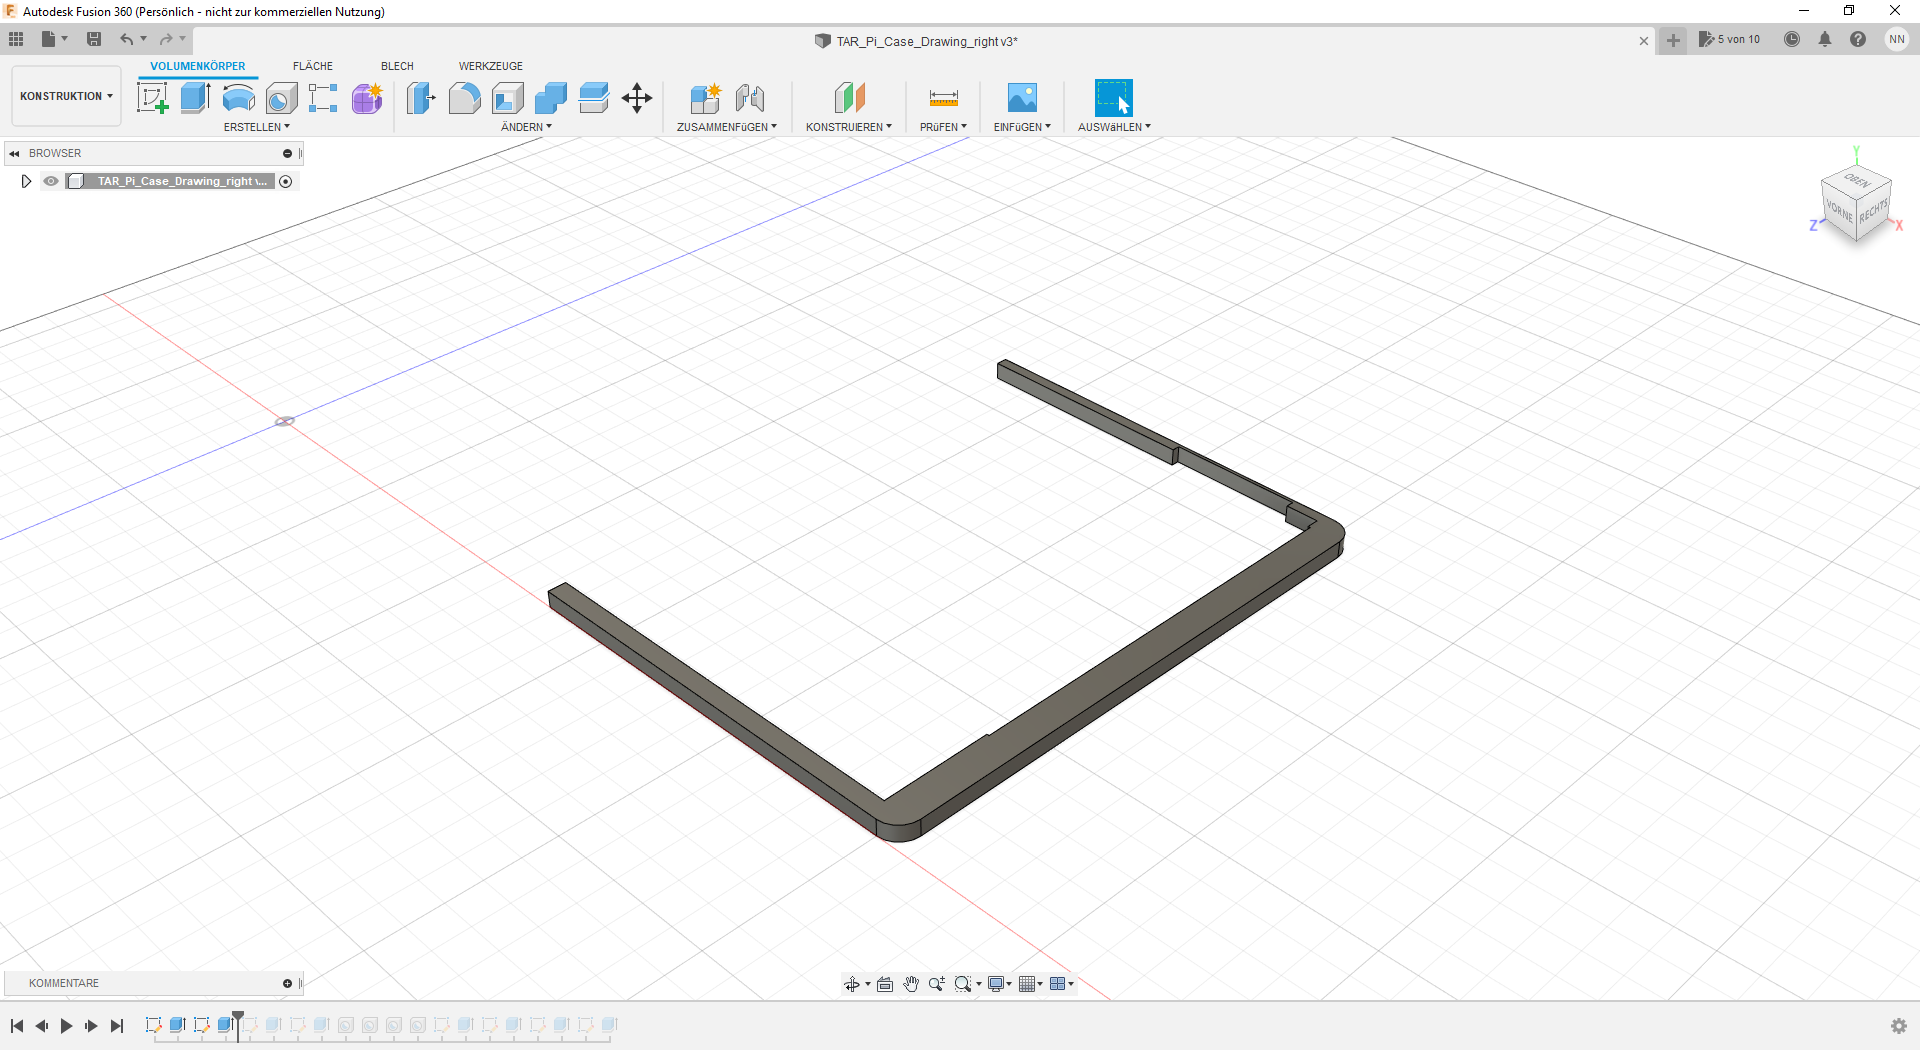
\includegraphics[width=\linewidth]{img/konstruktion_gehaeuse_rechts_003.png}
		\caption[]{}
		\label{fig:design-right-03}
	\end{subfigure}
	\begin{subfigure}[t]{.3\linewidth}
		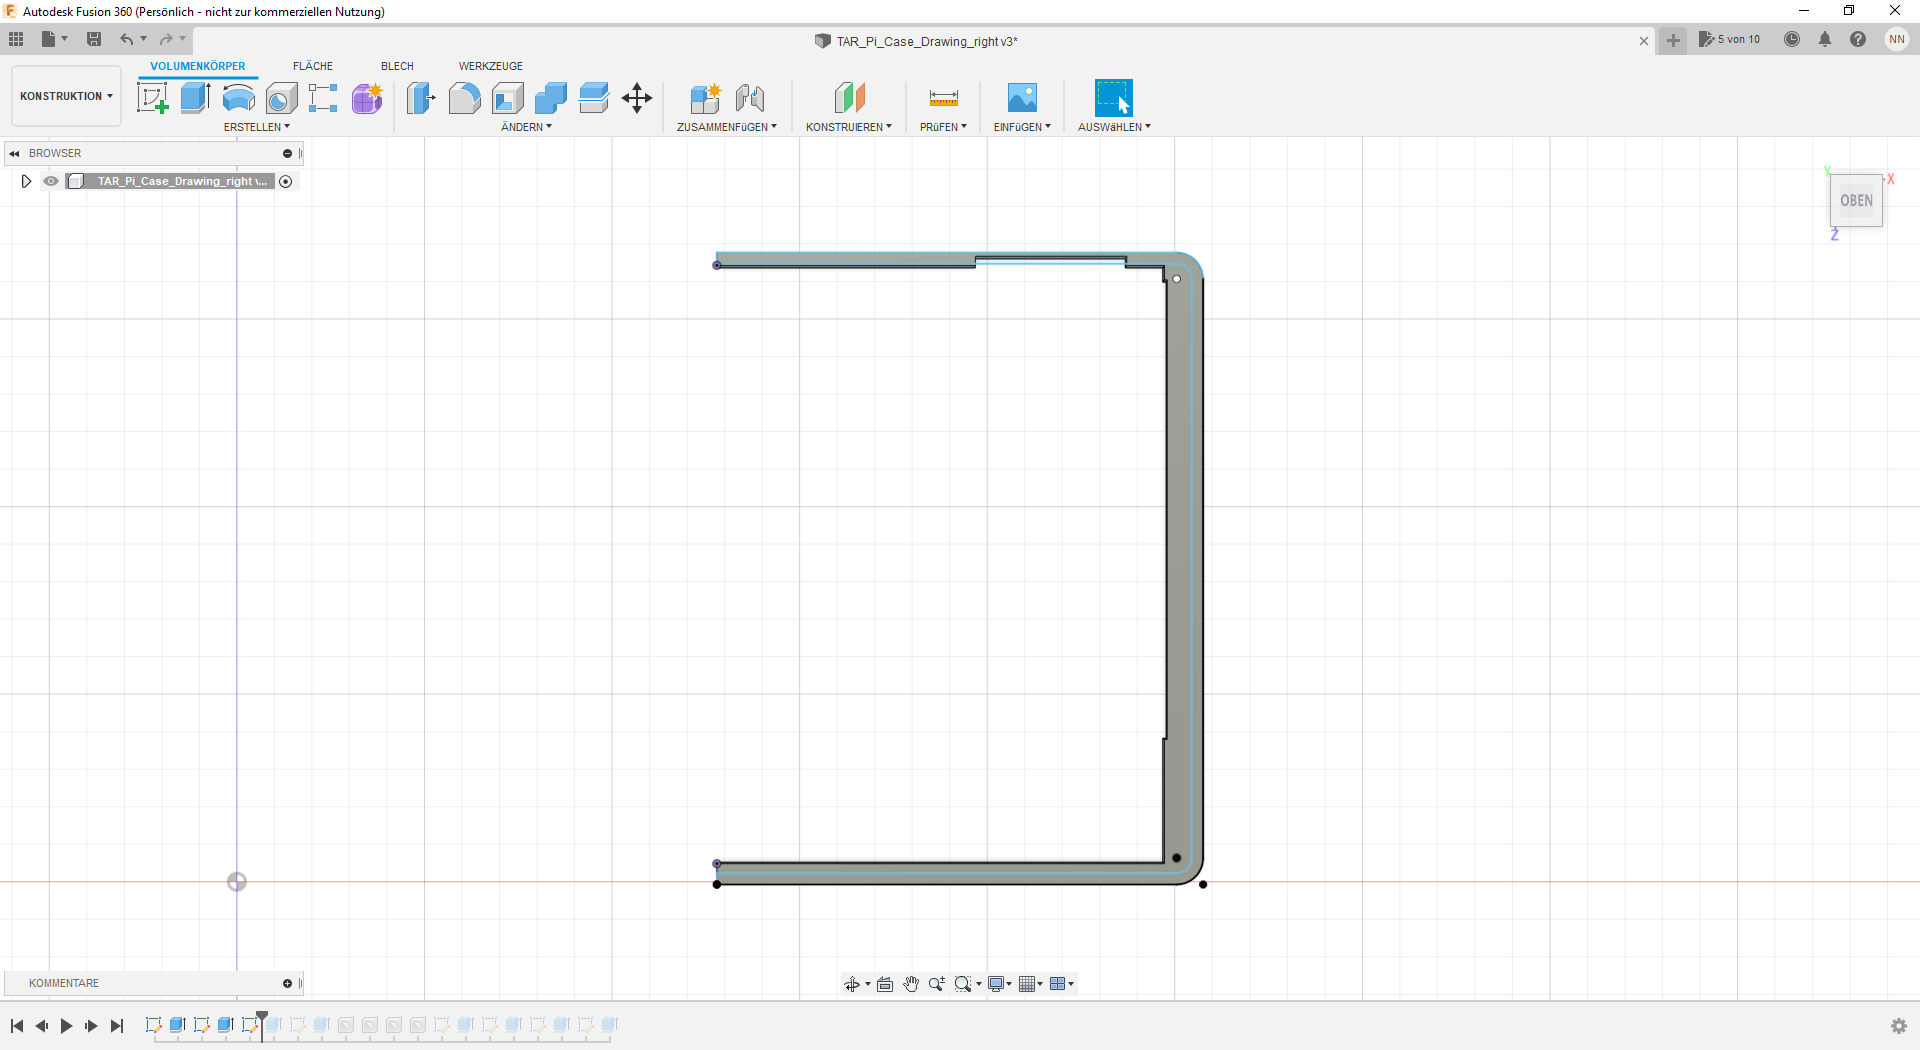
\includegraphics[width=\linewidth]{img/konstruktion_gehaeuse_rechts_004.png}
		\caption[]{}
		\label{fig:design-right-04}
	\end{subfigure}
	\begin{subfigure}[t]{.3\linewidth}
		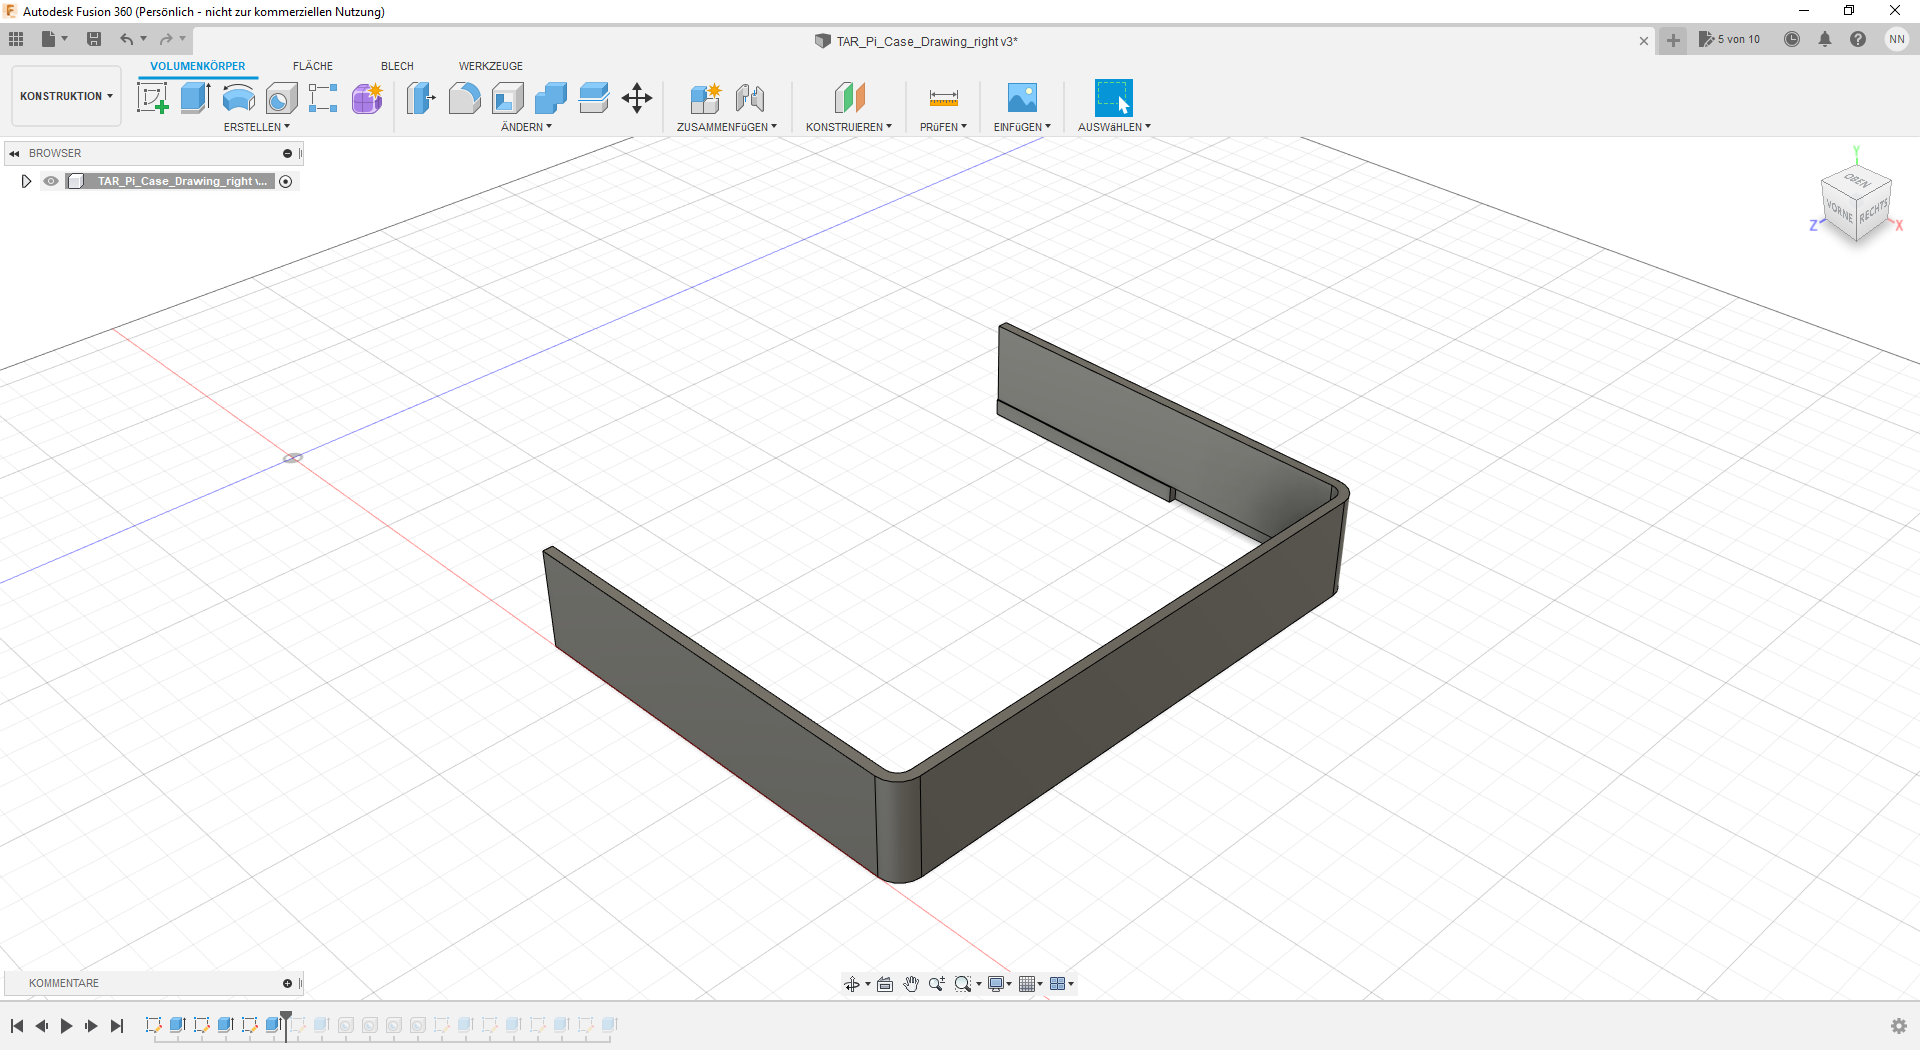
\includegraphics[width=\linewidth]{img/konstruktion_gehaeuse_rechts_005.png}
		\caption[]{}
		\label{fig:design-right-05}
	\end{subfigure}
	\begin{subfigure}[t]{.3\linewidth}
		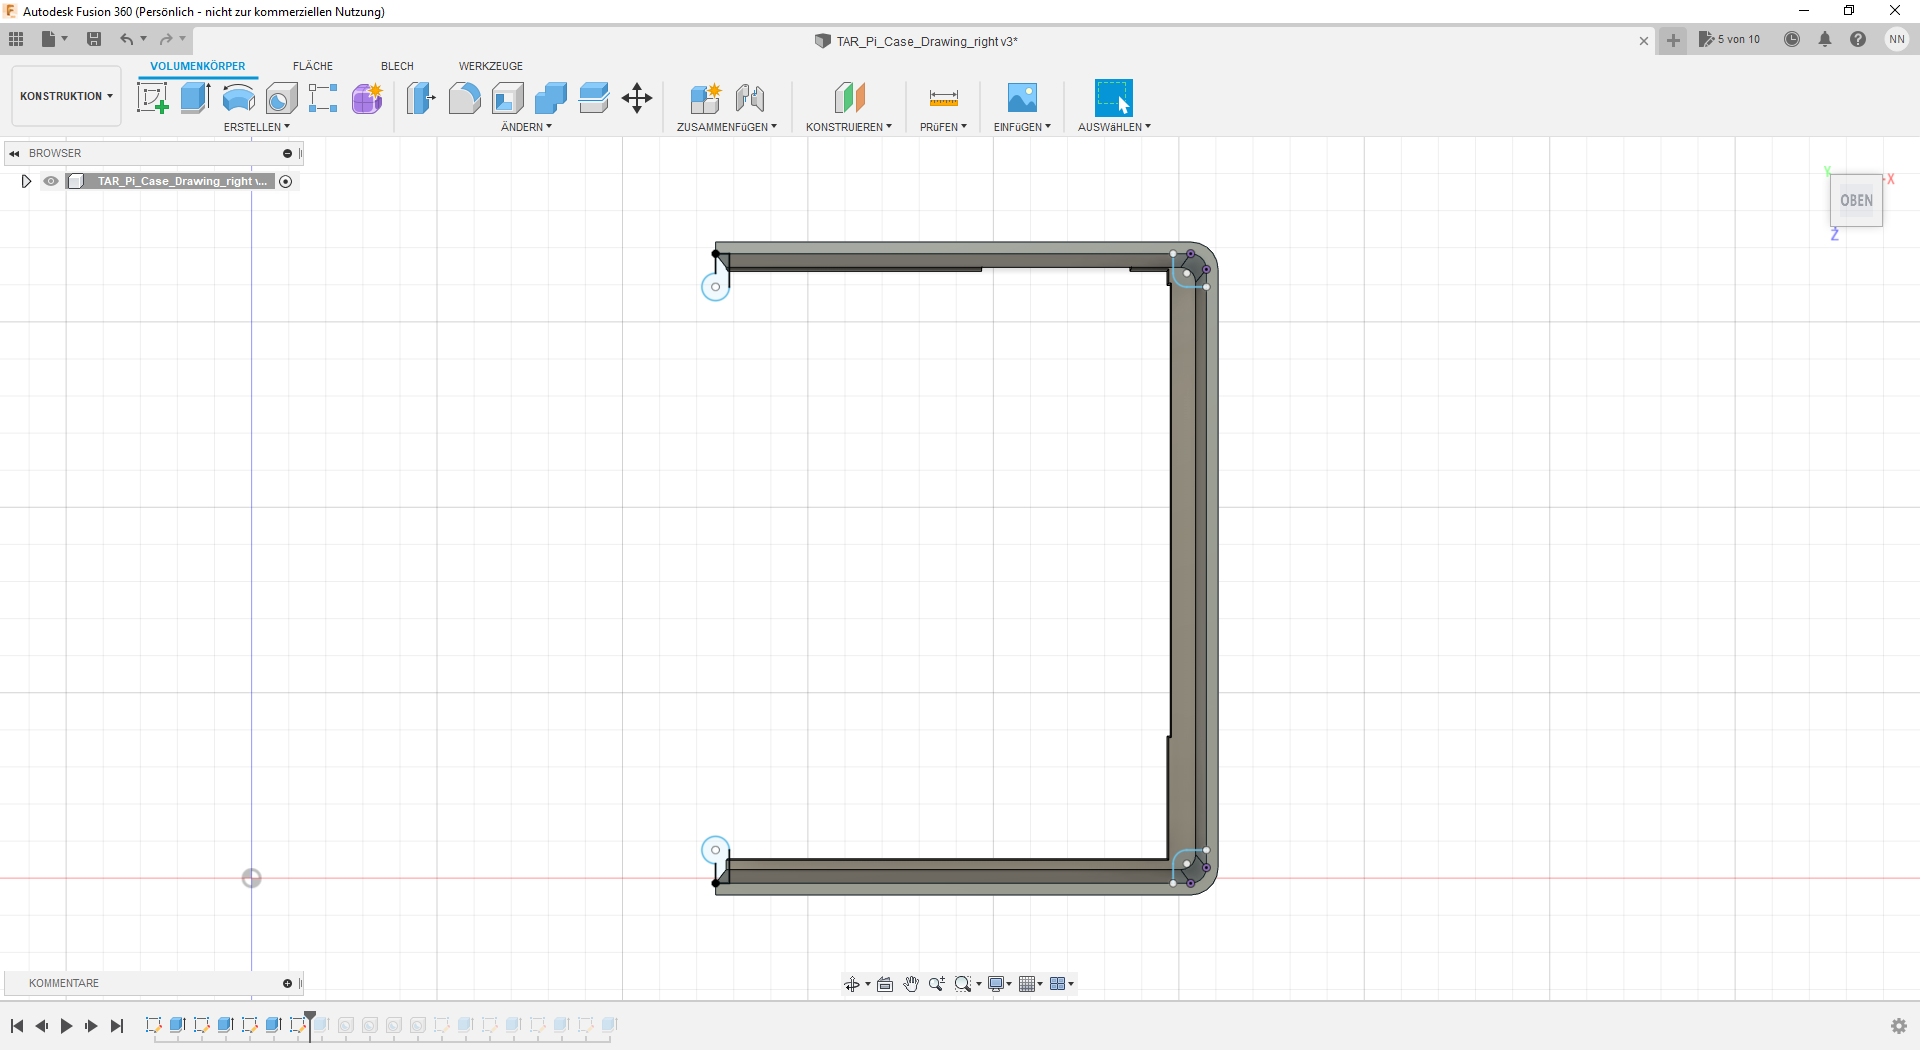
\includegraphics[width=\linewidth]{img/konstruktion_gehaeuse_rechts_006.png}
		\caption[]{}
		\label{fig:design-right-06}
	\end{subfigure}
	\begin{subfigure}[t]{.3\linewidth}
		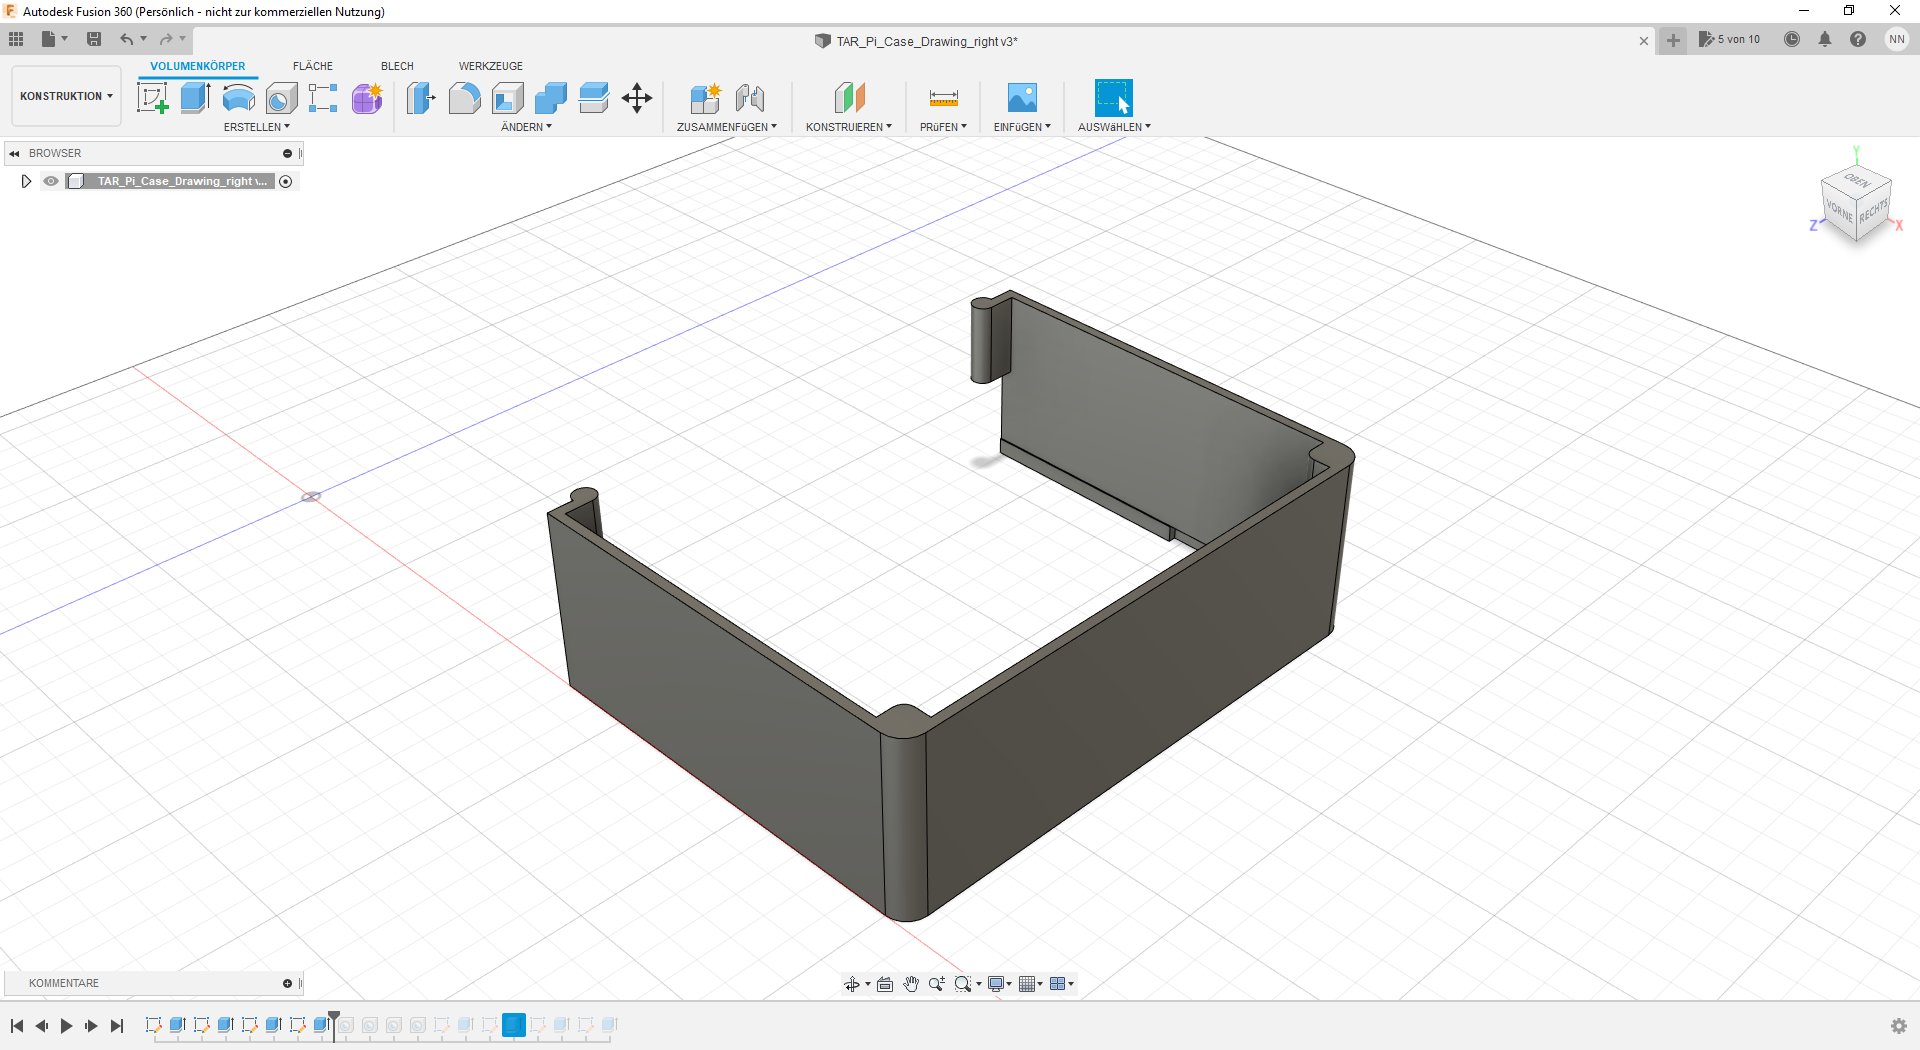
\includegraphics[width=\linewidth]{img/konstruktion_gehaeuse_rechts_007.png}
		\caption[]{}
		\label{fig:design-right-07}
	\end{subfigure}
	\begin{subfigure}[t]{.3\linewidth}
		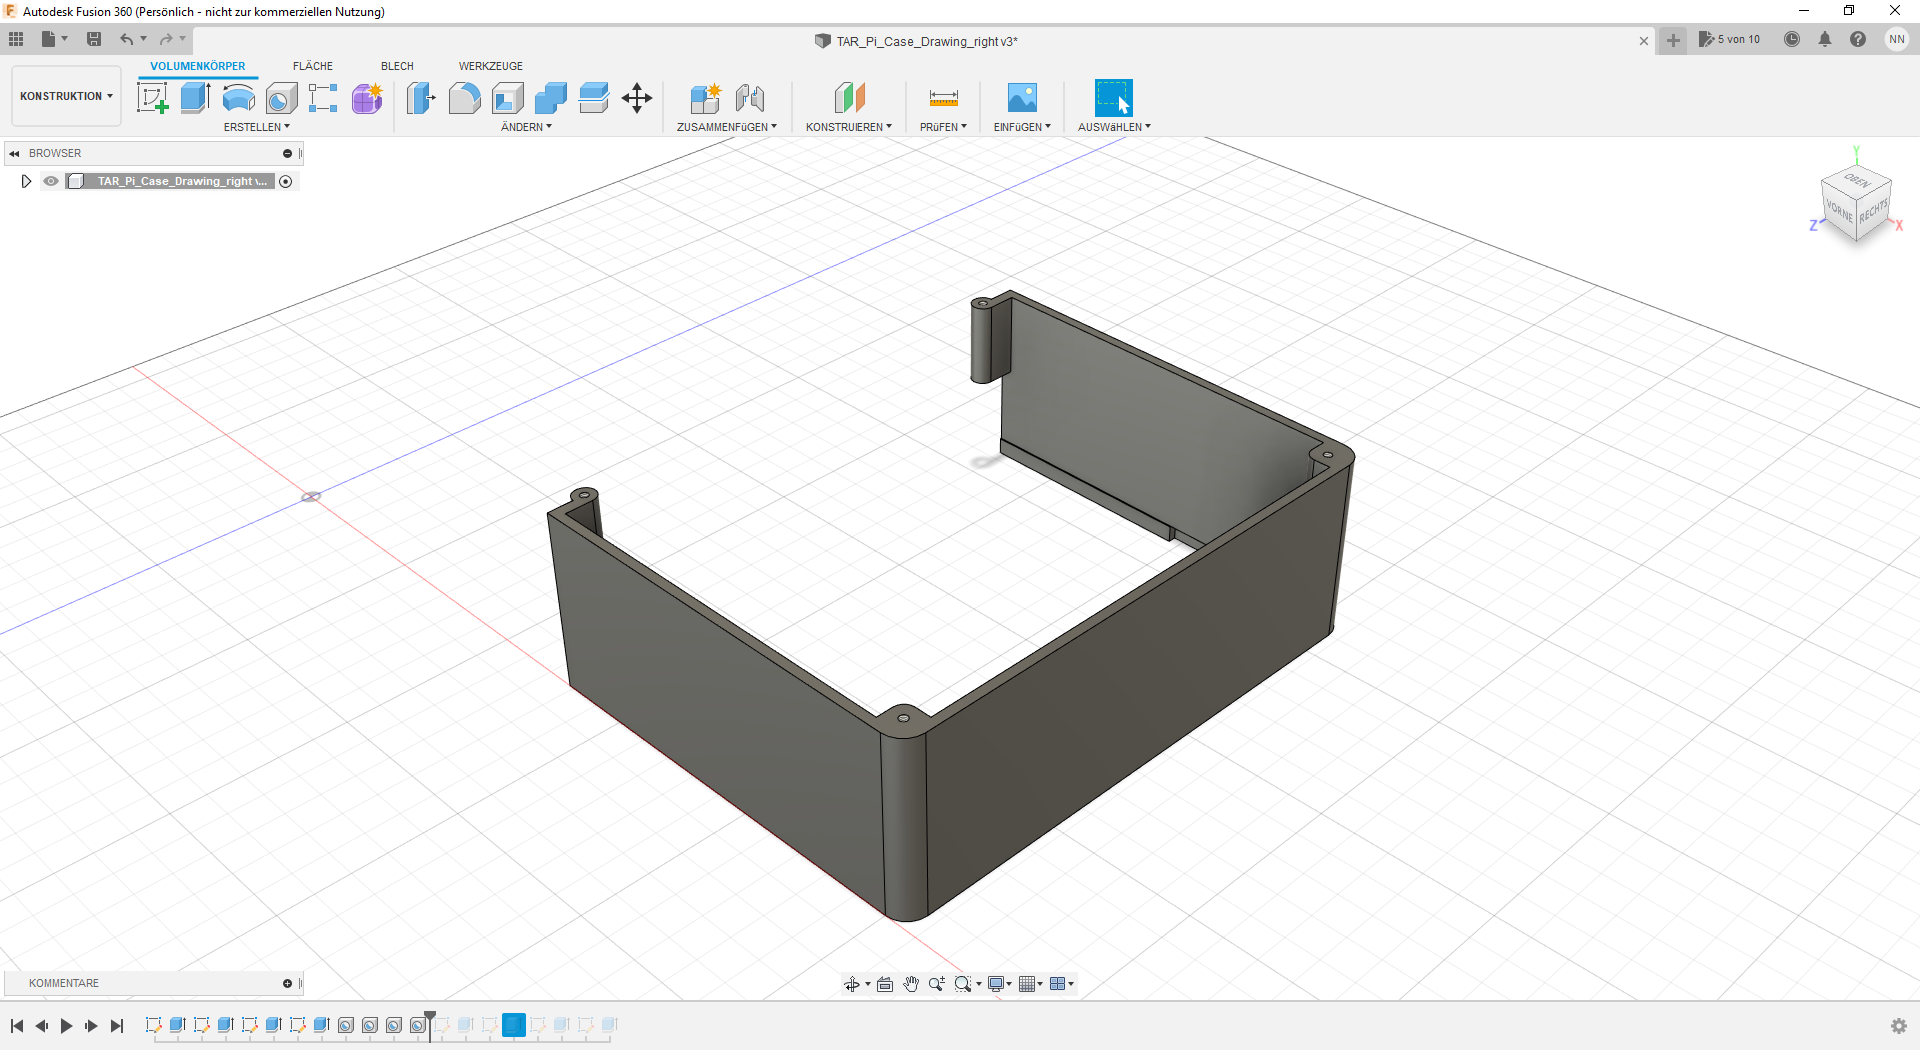
\includegraphics[width=\linewidth]{img/konstruktion_gehaeuse_rechts_008.png}
		\caption[]{}
		\label{fig:design-right-08}
	\end{subfigure}
	\begin{subfigure}[t]{.3\linewidth}
		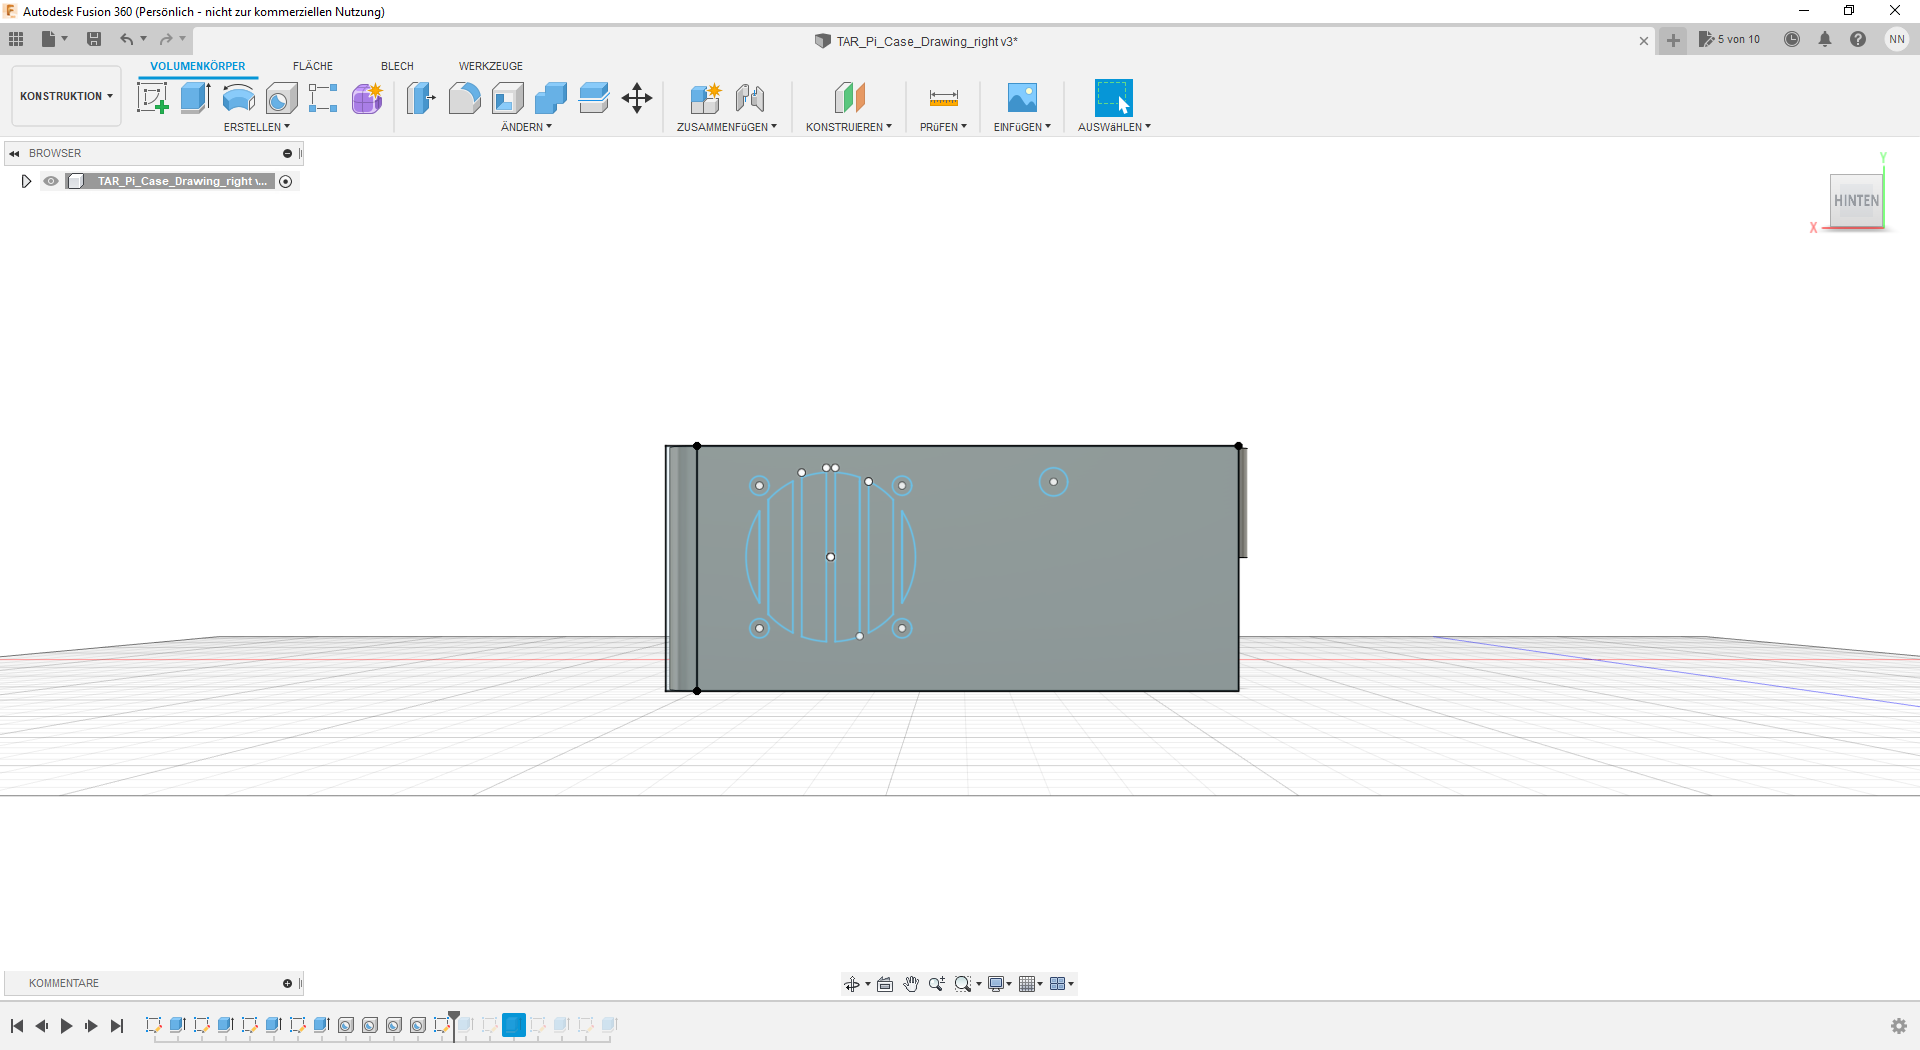
\includegraphics[width=\linewidth]{img/konstruktion_gehaeuse_rechts_009.png}
		\caption[]{}
		\label{fig:design-right-09}
	\end{subfigure}
	\begin{subfigure}[t]{.3\linewidth}
		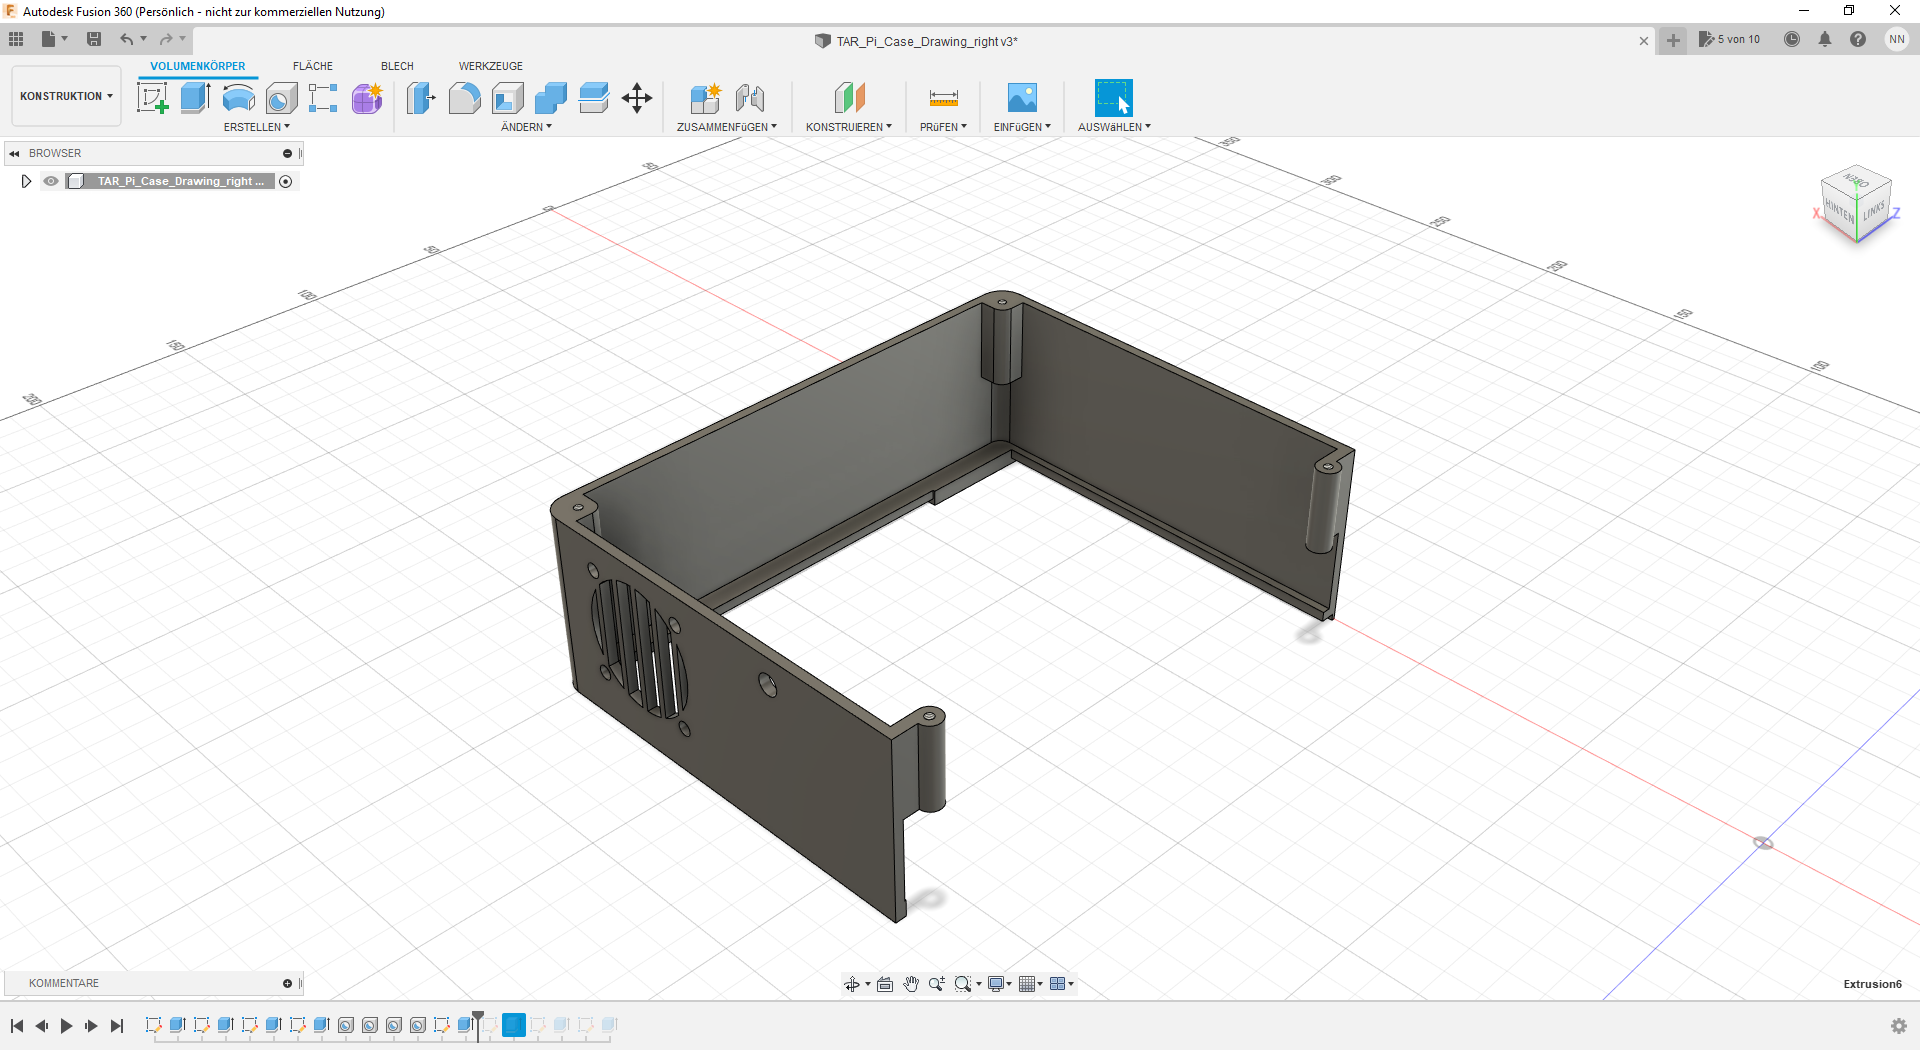
\includegraphics[width=\linewidth]{img/konstruktion_gehaeuse_rechts_010.png}
		\caption[]{}
		\label{fig:design-right-10}
	\end{subfigure}
	\begin{subfigure}[t]{.3\linewidth}
		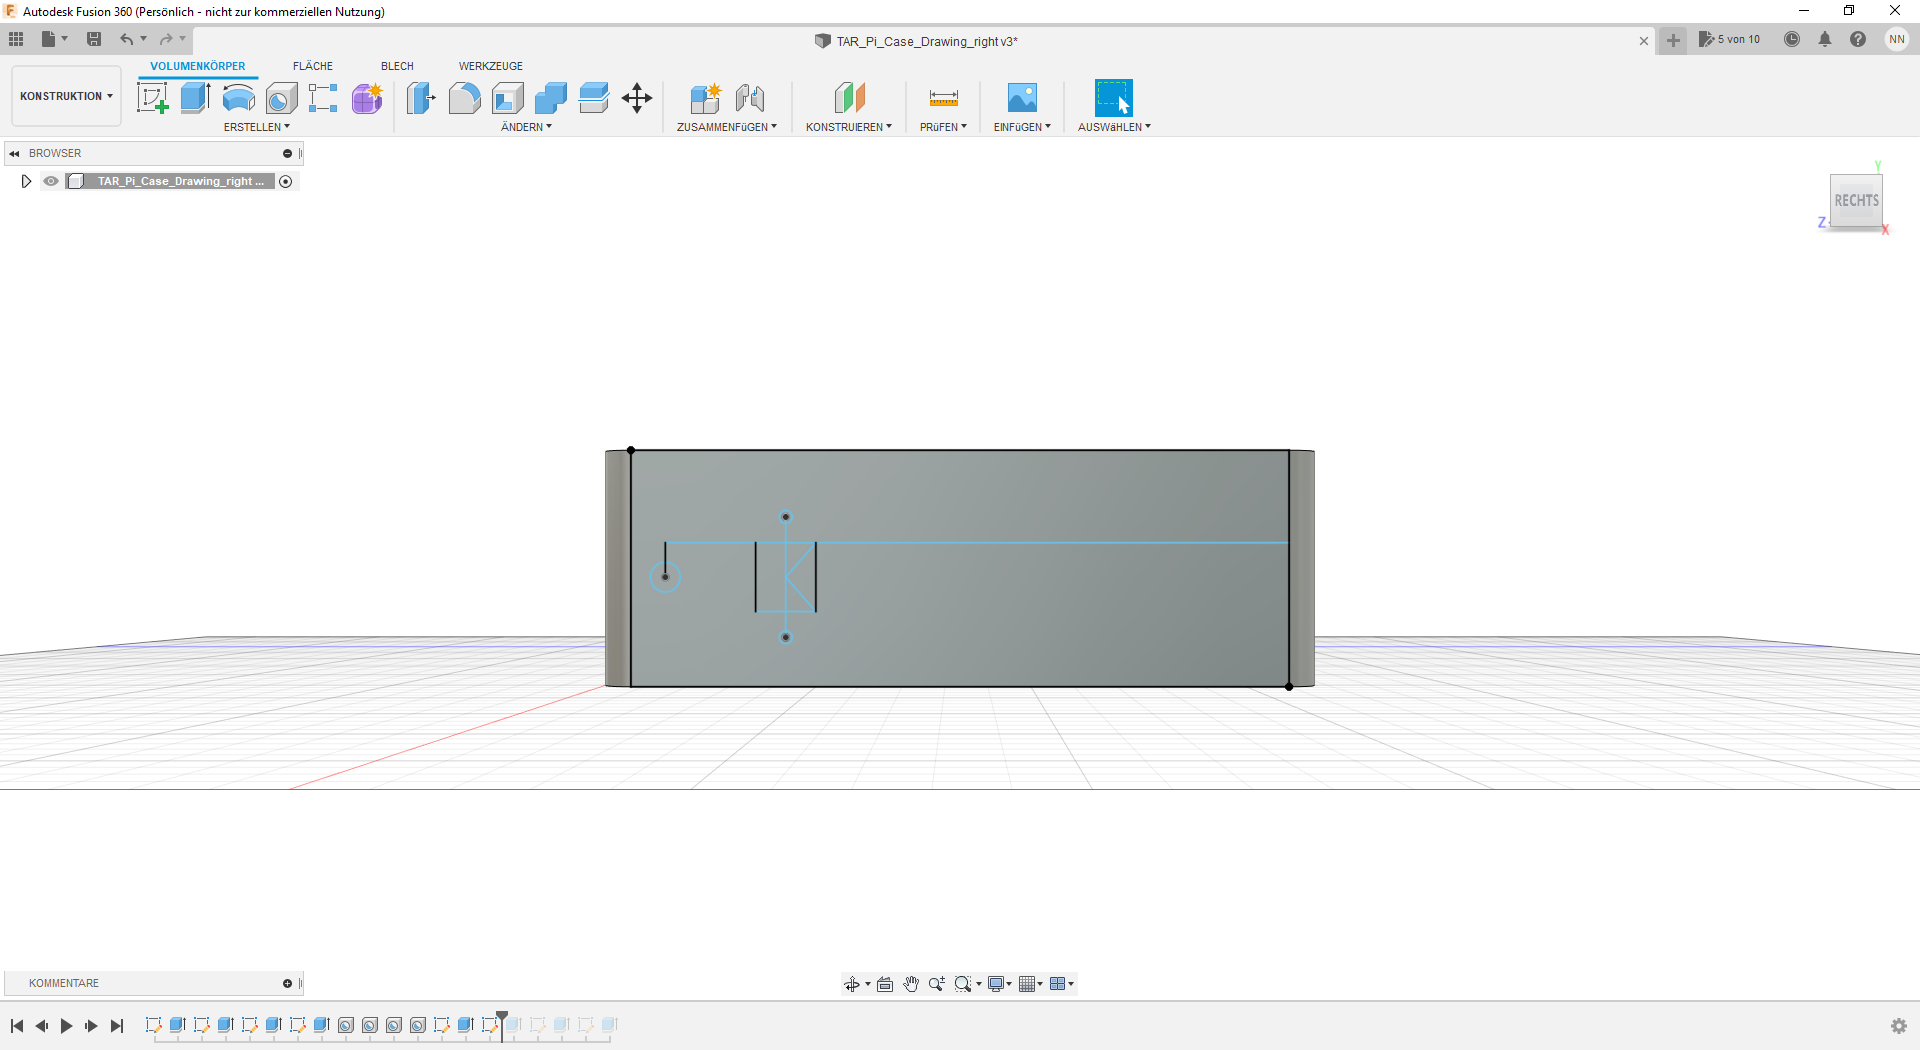
\includegraphics[width=\linewidth]{img/konstruktion_gehaeuse_rechts_011.png}
		\caption[]{}
		\label{fig:design-right-11}
	\end{subfigure}
	\begin{subfigure}[t]{.3\linewidth}
		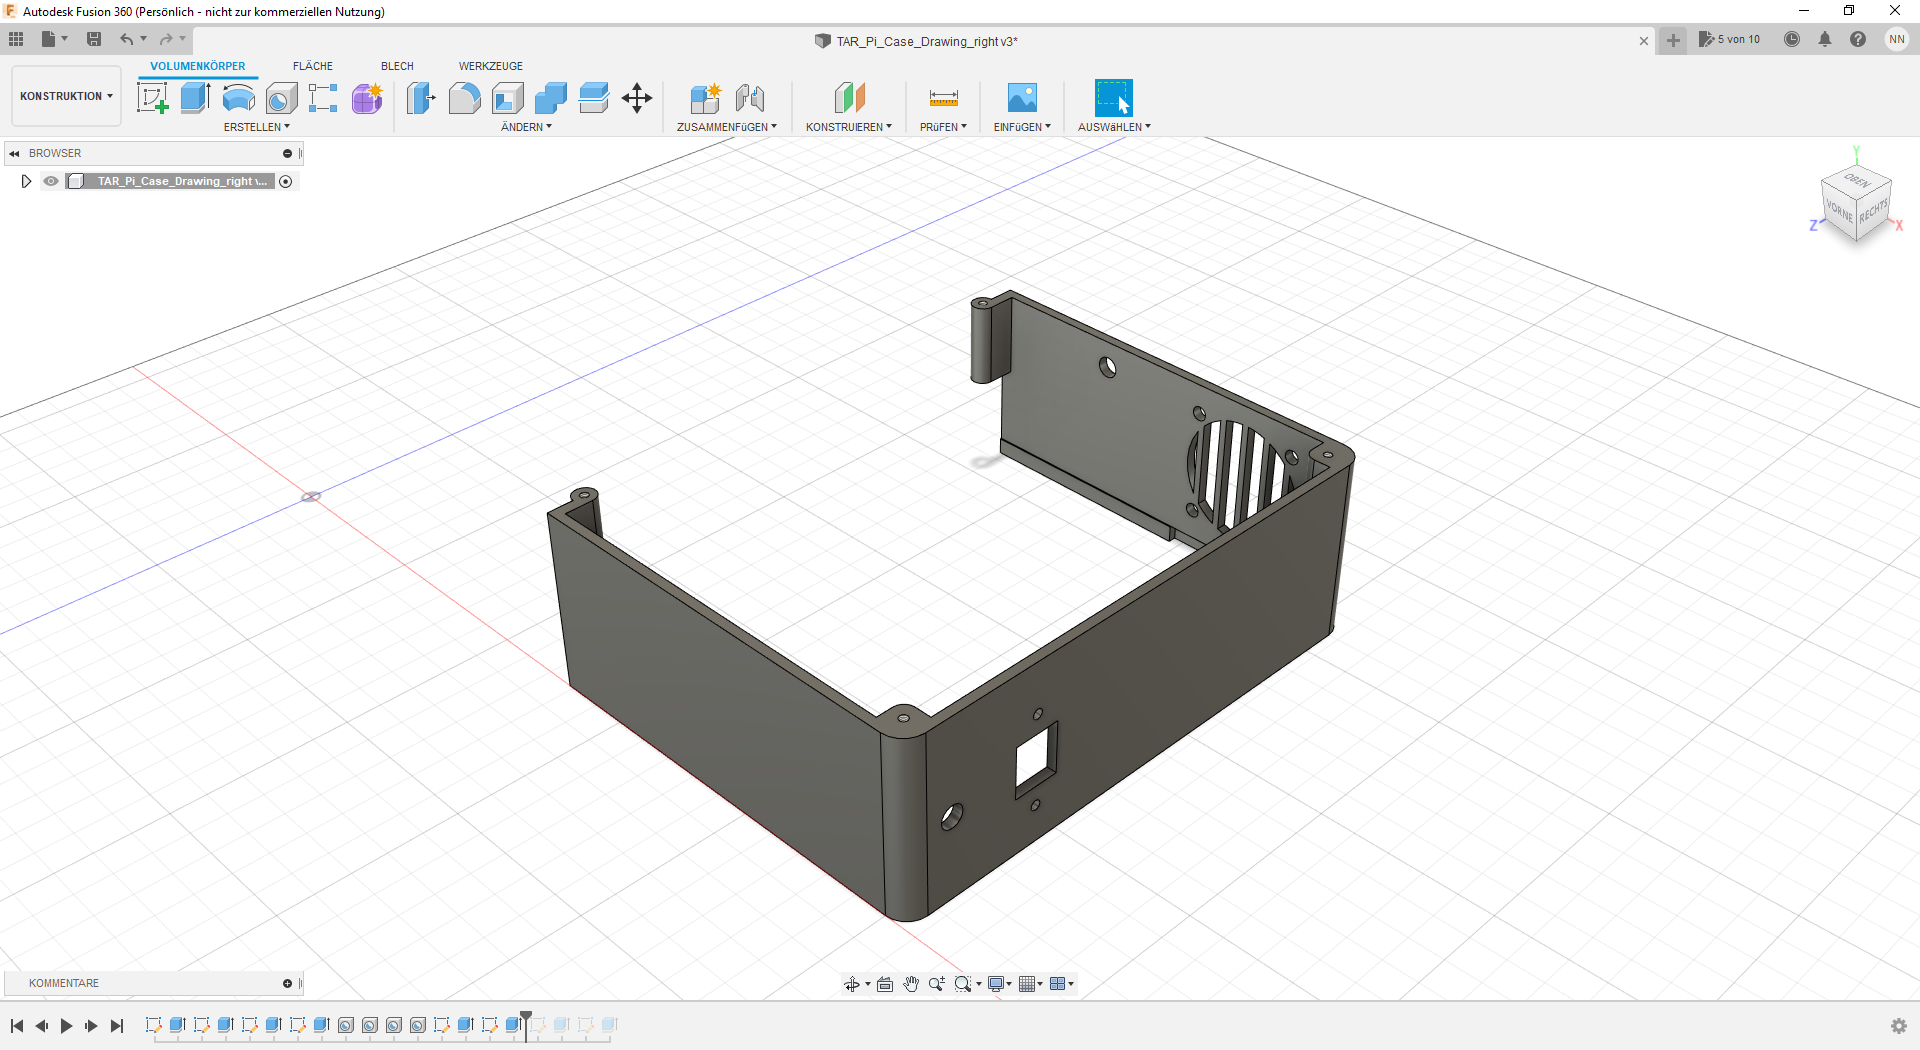
\includegraphics[width=\linewidth]{img/konstruktion_gehaeuse_rechts_012.png}
		\caption[]{}
		\label{fig:design-right-12}
	\end{subfigure}
	\begin{subfigure}[t]{.3\linewidth}
		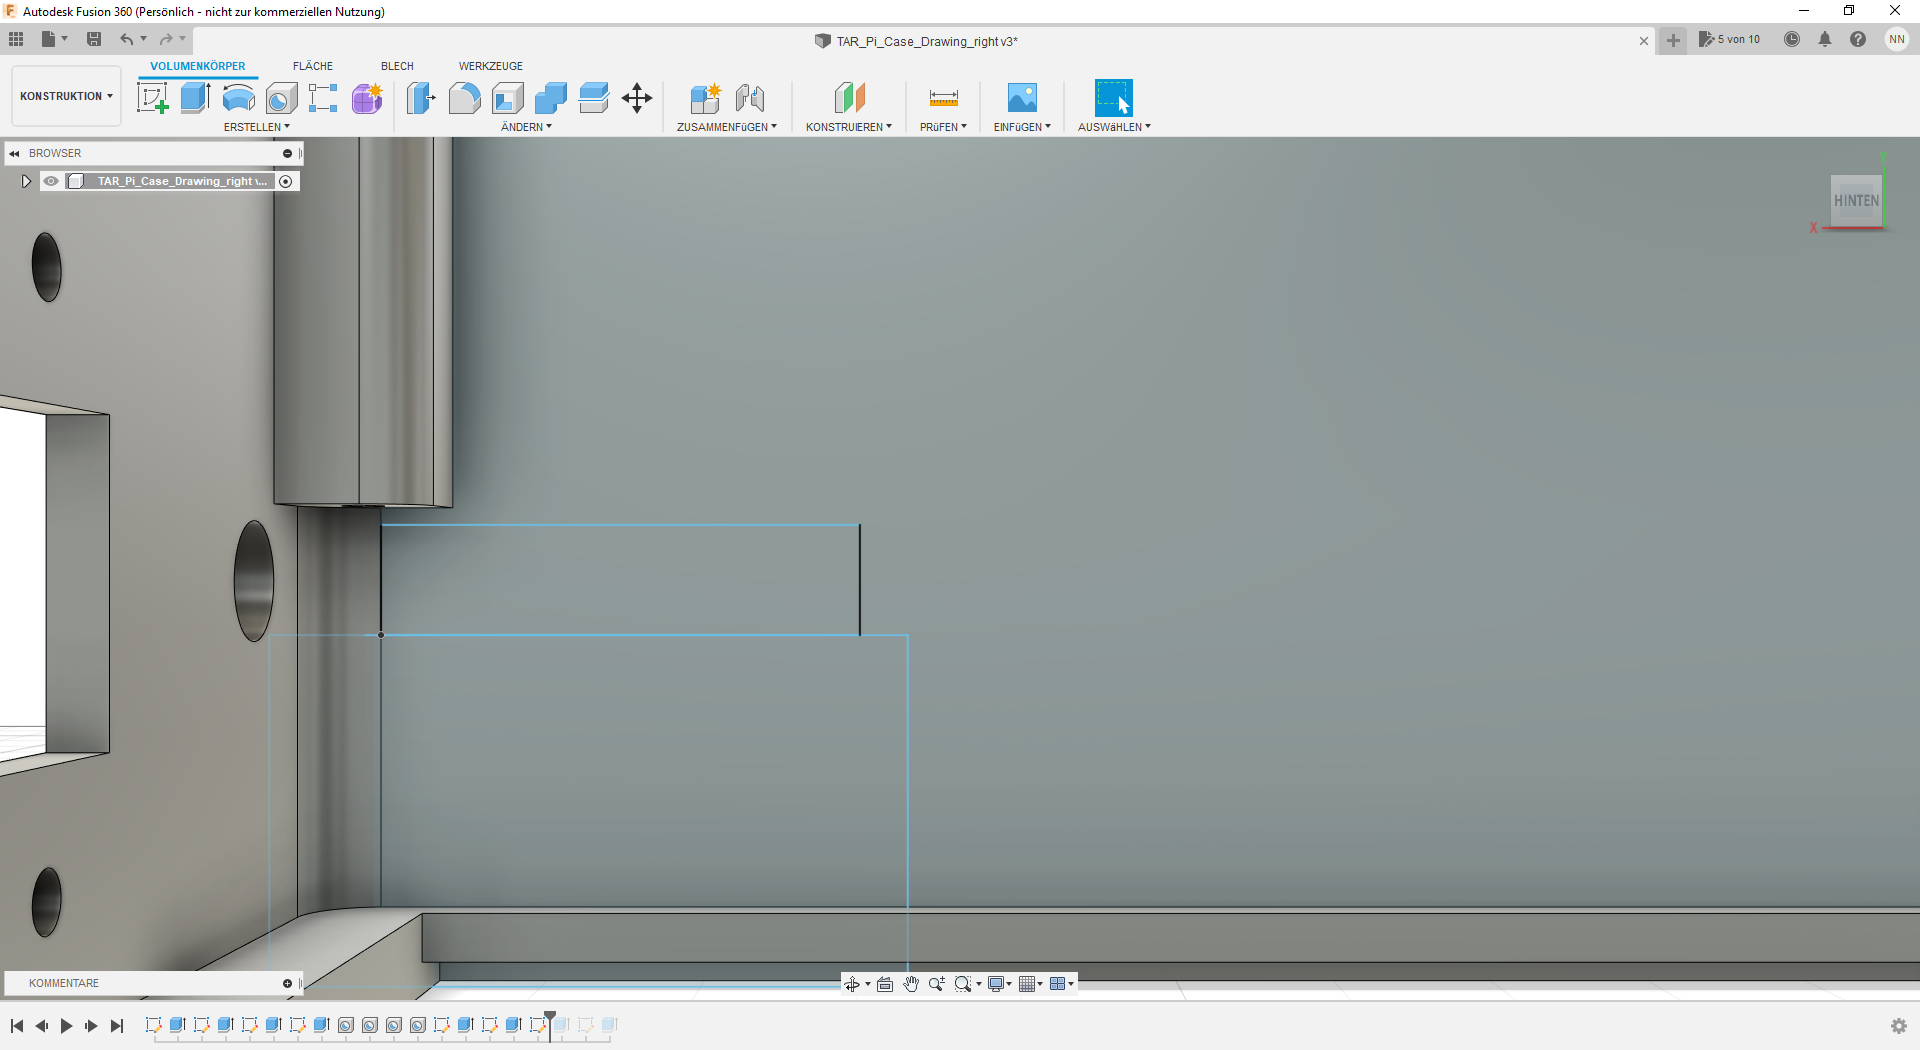
\includegraphics[width=\linewidth]{img/konstruktion_gehaeuse_rechts_013.png}
		\caption[]{}
		\label{fig:design-right-13}
	\end{subfigure}
	\begin{subfigure}[t]{.3\linewidth}
		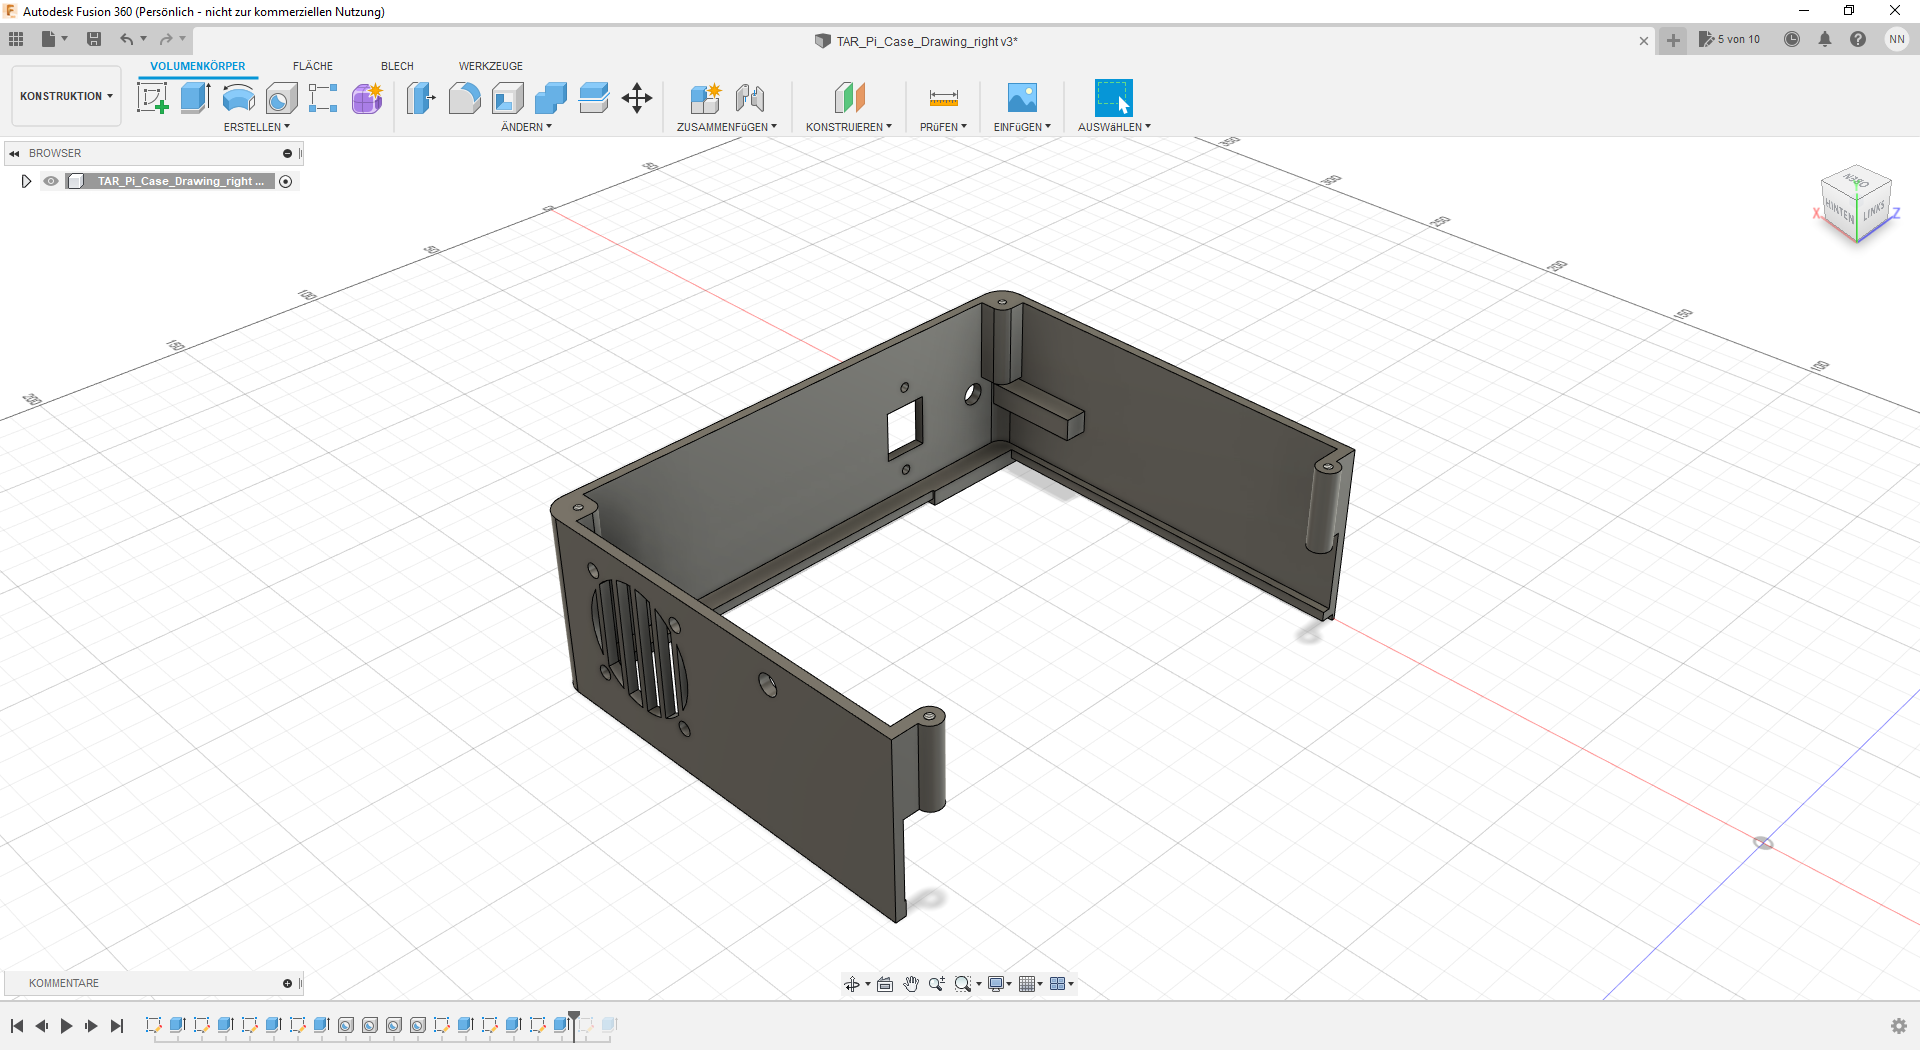
\includegraphics[width=\linewidth]{img/konstruktion_gehaeuse_rechts_014.png}
		\caption[]{}
		\label{fig:design-right-14}
	\end{subfigure}
	\begin{subfigure}[t]{.3\linewidth}
		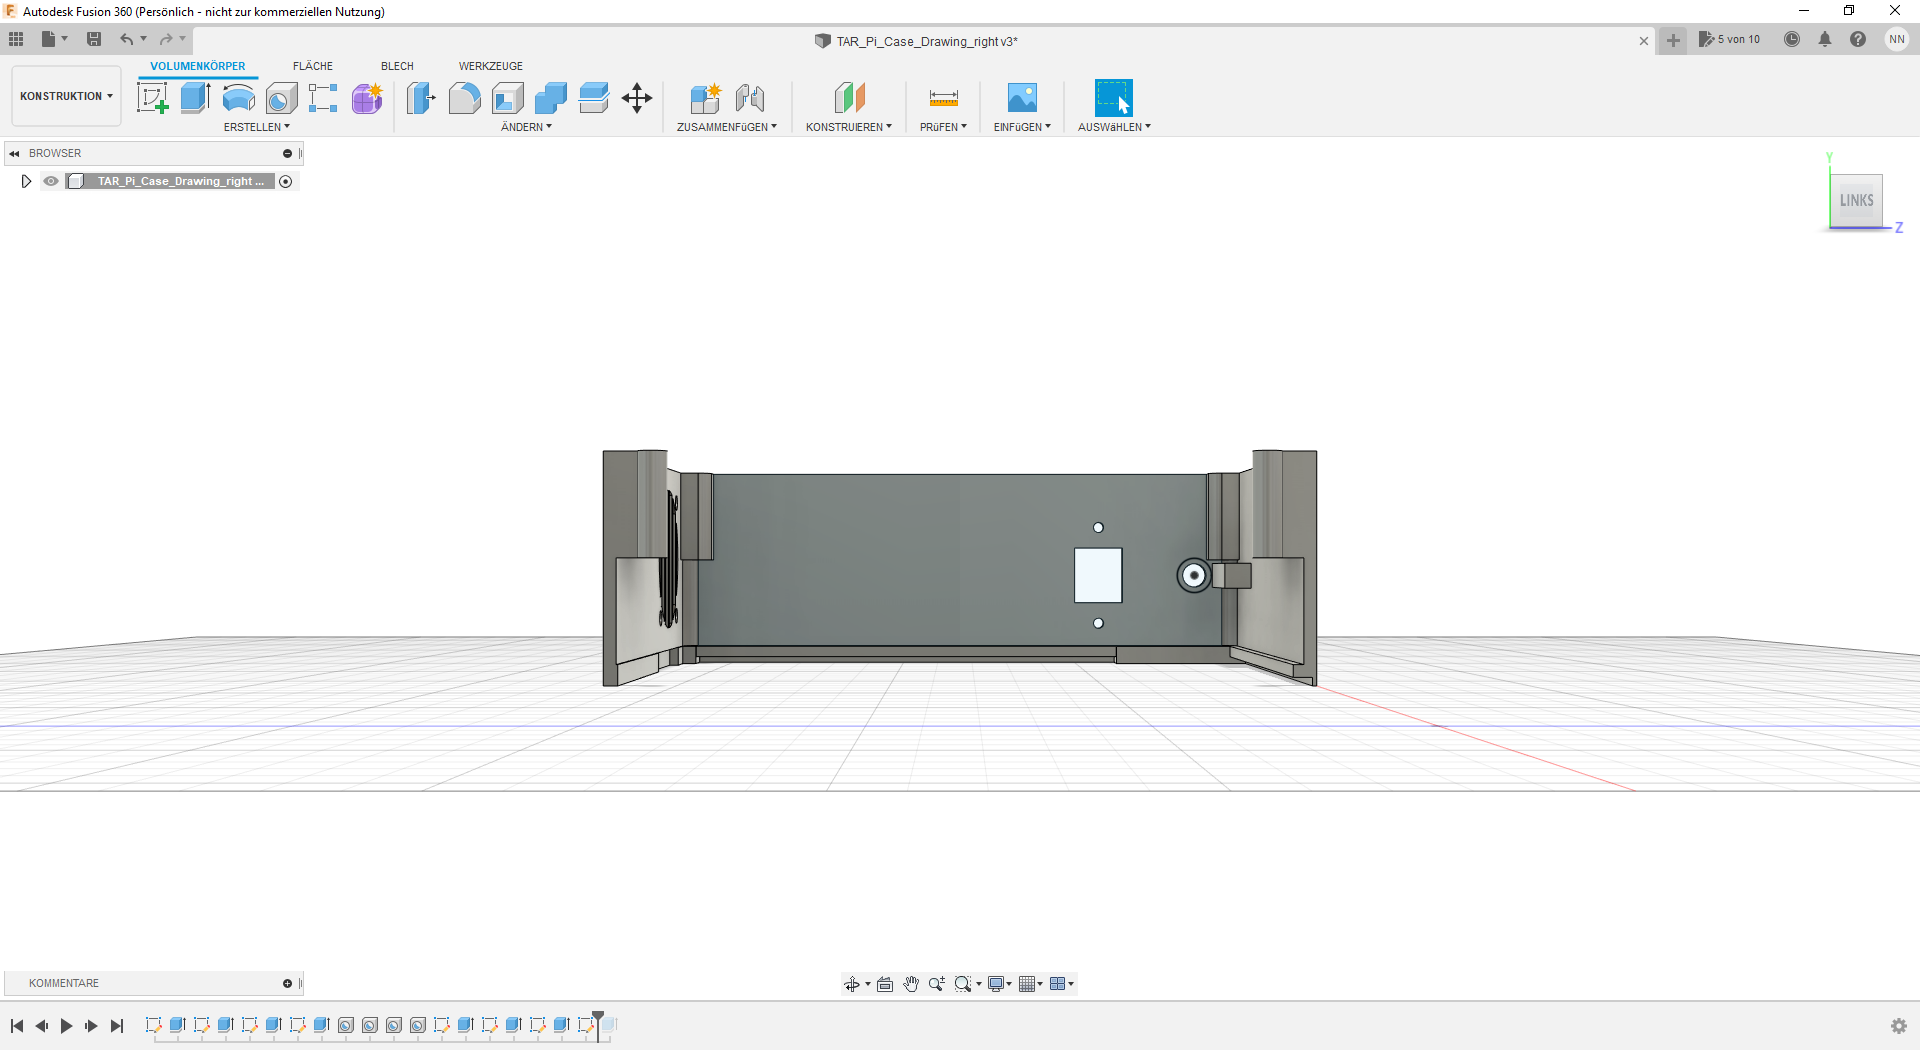
\includegraphics[width=\linewidth]{img/konstruktion_gehaeuse_rechts_015.png}
		\caption[]{}
		\label{fig:design-right-15}
	\end{subfigure}
	\begin{subfigure}[t]{.3\linewidth}
		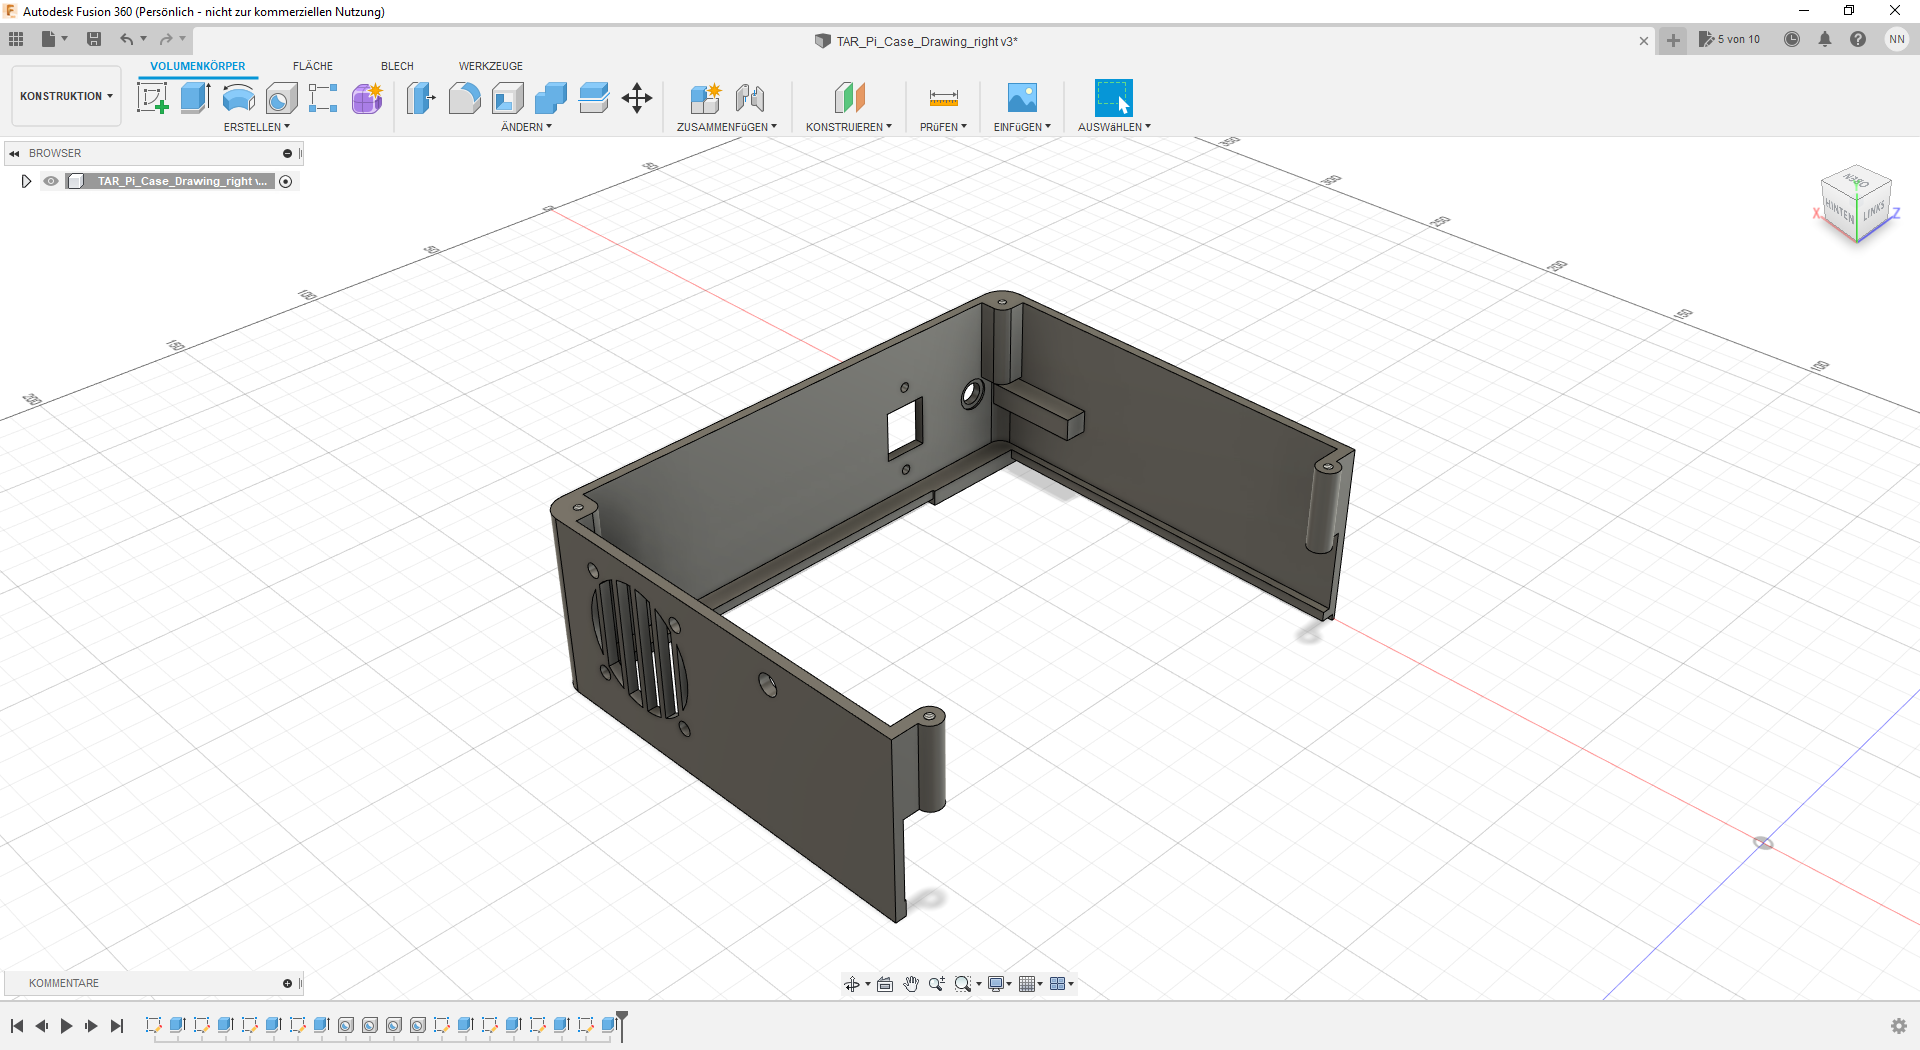
\includegraphics[width=\linewidth]{img/konstruktion_gehaeuse_rechts_016.png}
		\caption[]{}
		\label{fig:design-right-16}
	\end{subfigure}
	\caption[Entwurf des rechten Wandteils]{Entwurf des rechten Wandteils}
	\label{fig:design-right}
\end{figure}\par
\newpage
\paragraph{Gehäuserückwand}
Das Design der Gehäuserückwand basiert nur rudimentär auf der in \ref{fig:design-case-base} erstellten Zeichnung. Die Außenmaße Stimmen zwar überein, die Zeichnung für die Auflage auf den Seitenwänden musste aber neu erstellt werden. Zusätzlich wurde eine Diagonale zur punktsymmetrischen Trennung der Teile eingefügt (vgl. \ref{fig:design-back-01}), welche die Zeit für die Konstruktion von zwei unterschiedlichen Teilen für die Rückseite reduzieren soll. Die Zeichnung wurde dann entsprechend extrudiert (vgl. \ref{fig:design-back-02}). Um die Teile nach dem Druck besser verbinden zu können, wurde ein Vorsprung auf der kurzen Seite des Bauteils extruiert (vgl. \ref{fig:design-back-03}). Um beim Druck Material zu sparen, wurde ein weiter Teil der Innenzeichnung ins Negative extruiert, um den Bereich freizustellen (vgl. \ref{fig:design-back-04}). Für evetuelle Toleranzen zwischen den beiden Teilen wurde auf dem Vorsprung die Aussparung für die unterliegende Schraubendurchführung erhöht (vgl. \ref{fig:design-back-05}). Zusätzlich wurde der Vorsprung von unten mit einer Phase versehen, um die Materialnutzung für das Teil weiter zu reduzieren (vgl. \ref{fig:design-back-06}). Des weiteren wurde an die obere Kante (vgl. \ref{fig:design-back-07}) und an die Innenkante (vgl. \ref{fig:design-back-08}) mit einer Phase versehen. Eine ähnliche Phase wurde auch an dem Vorsprung angebracht (vgl. \ref{fig:design-back-09}). Um die Bohrung am die richtige Stelle zu setzen, wurde eine Hilfzeichnung auf die Außenfläche gesetzt (vgl. \ref{fig:design-back-10}). Anschließend wurden drei M3-Bohrungen für Senkkopfschrauben gesetzt (vgl. \ref{fig:design-back-11}). Um das Gehäuse an der Wand anbringen zu können, wurden eine Zeichnung auf die Oberseite des Gehäuses gelegt (vgl. \ref{fig:design-back-12}) und dann ins Negativ extruiert (vgl. \ref{fig:design-back-13}. Um bei der Anbringung nicht an einen bestimmten Typ Schrauben gebunden zu sein, wurde eine kleine Phase an den engen Teil der Aufhängungslöcher gelegt (vgl. \ref{fig:design-back-14}). Damit bei der Verbindung der beiden Einzelteile die Vorsprünge nicht aneinander stoßen, wurde an den Vorsprung auch eine Phase angelegt (vgl. \ref{fig:design-back-15}).
\begin{figure}[h!tb]
	\begin{subfigure}[t]{.3\linewidth}
		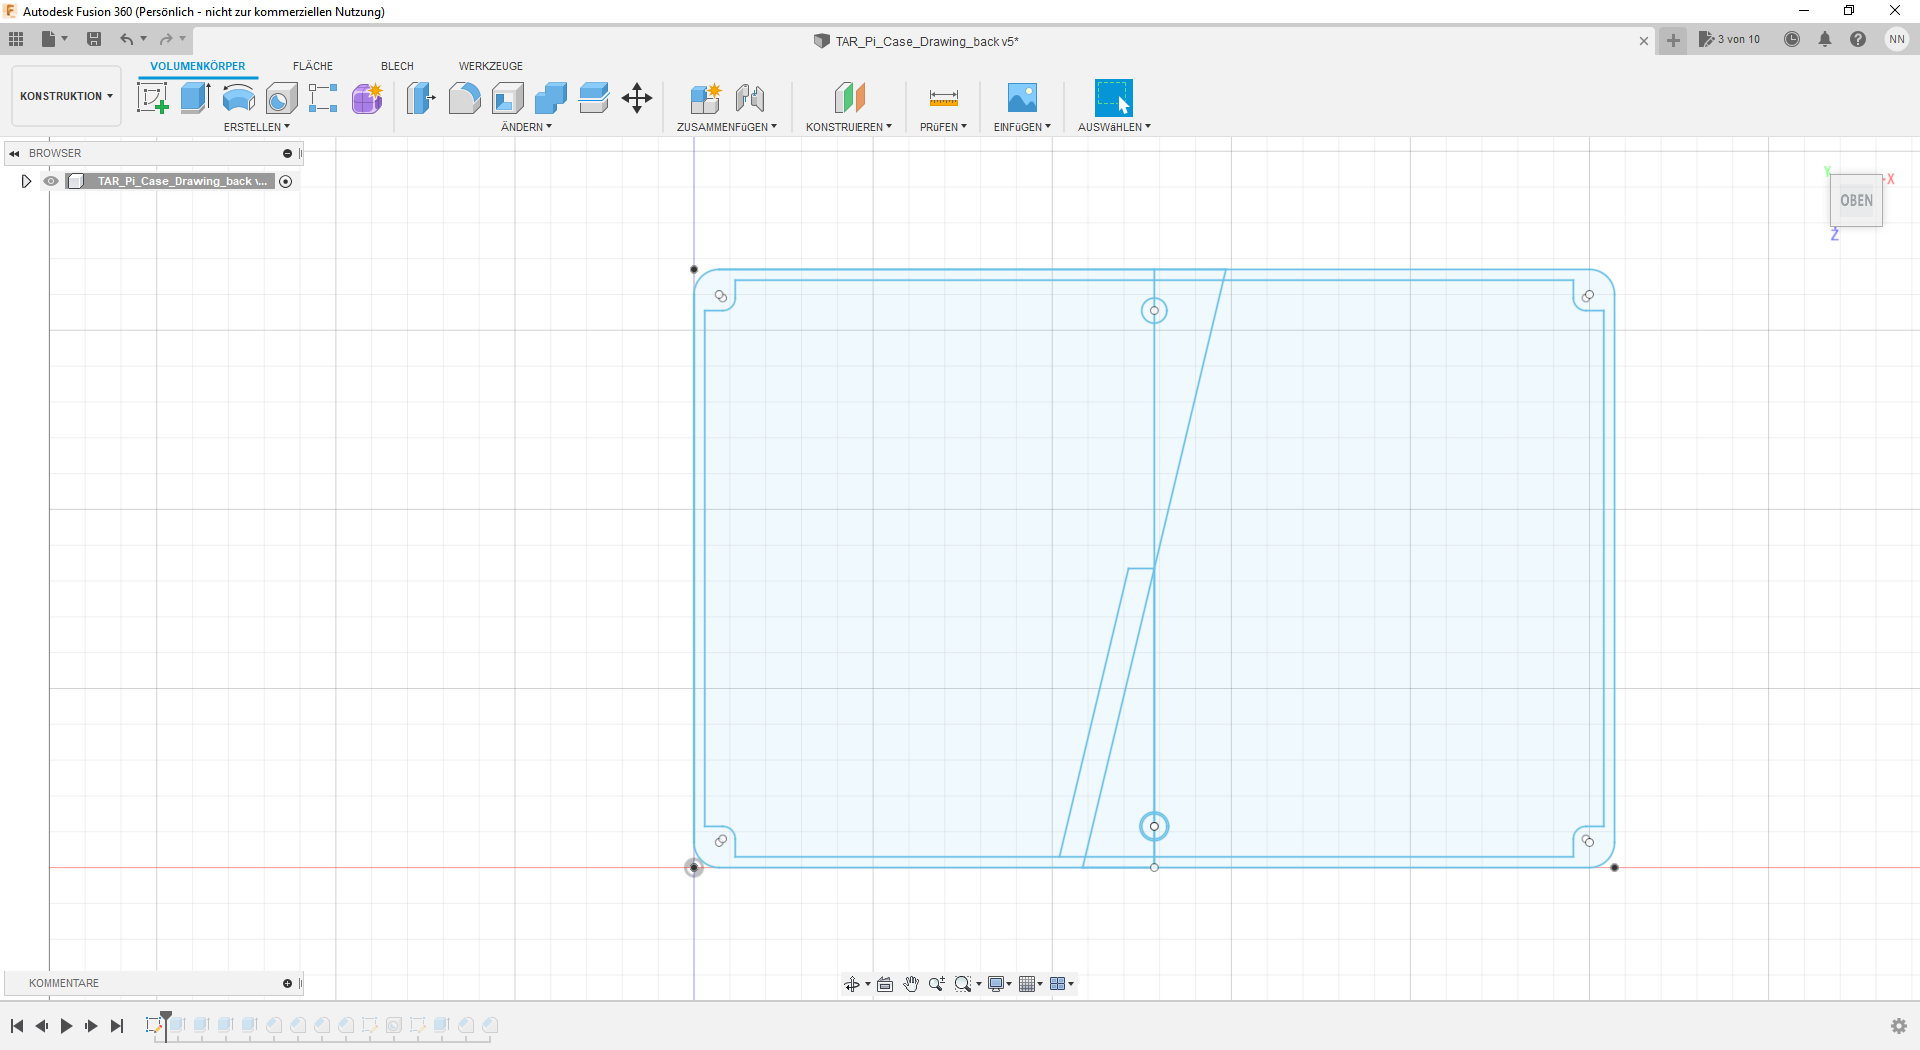
\includegraphics[width=\linewidth]{img/konstruktion_gehaeuse_hinten_001.png}
		\caption[]{}
		\label{fig:design-back-01}
	\end{subfigure}	
	\begin{subfigure}[t]{.3\linewidth}
		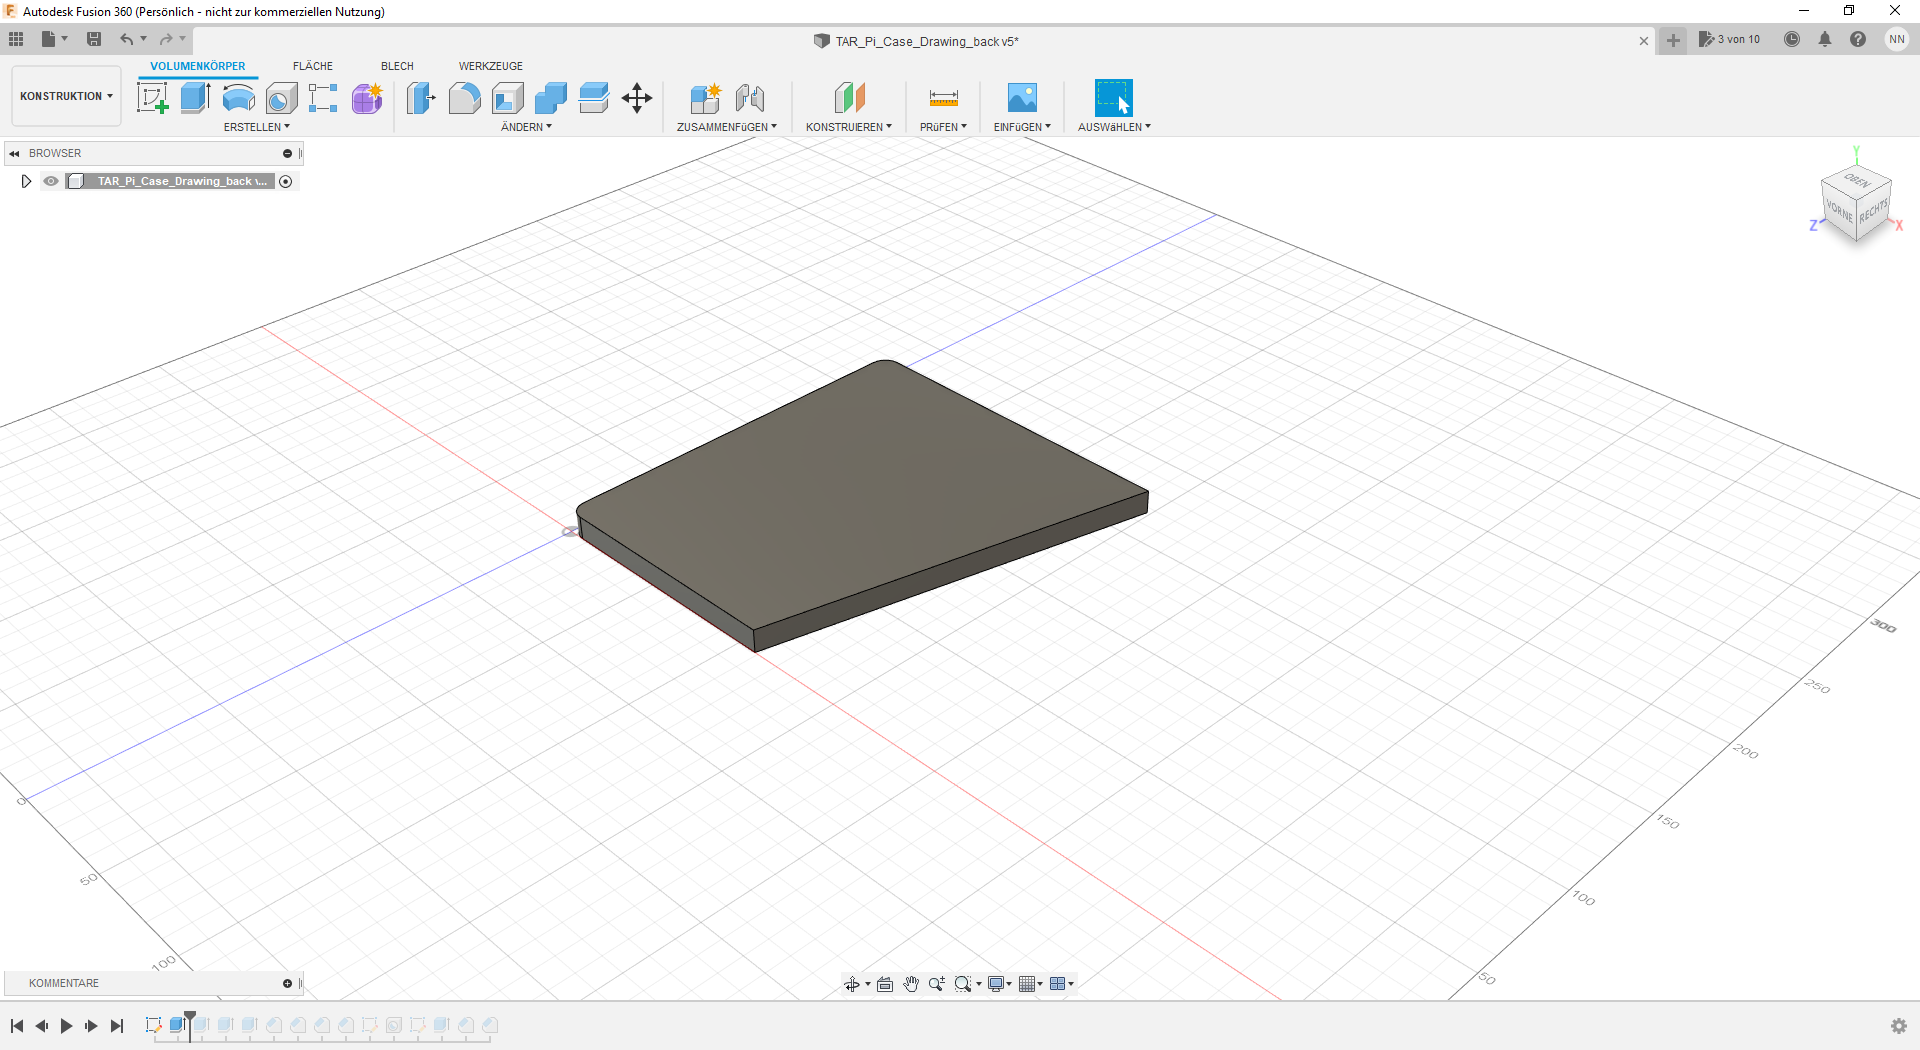
\includegraphics[width=\linewidth]{img/konstruktion_gehaeuse_hinten_002.png}
		\caption[]{}
		\label{fig:design-back-02}
	\end{subfigure}
	\begin{subfigure}[t]{.3\linewidth}
		\includegraphics[width=\linewidth]{img/konstruktion_gehaeuse_hinten_003.png}
		\caption[]{}
		\label{fig:design-back-03}
	\end{subfigure}
	\begin{subfigure}[t]{.3\linewidth}
		\includegraphics[width=\linewidth]{img/konstruktion_gehaeuse_hinten_004.png}
		\caption[]{}
		\label{fig:design-back-04}
	\end{subfigure}
	\begin{subfigure}[t]{.3\linewidth}
		\includegraphics[width=\linewidth]{img/konstruktion_gehaeuse_hinten_005.png}
		\caption[]{}
		\label{fig:design-back-05}
	\end{subfigure}
	\begin{subfigure}[t]{.3\linewidth}
		\includegraphics[width=\linewidth]{img/konstruktion_gehaeuse_hinten_006.png}
		\caption[]{}
		\label{fig:design-back-06}
	\end{subfigure}
	\begin{subfigure}[t]{.3\linewidth}
		\includegraphics[width=\linewidth]{img/konstruktion_gehaeuse_hinten_007.png}
		\caption[]{}
		\label{fig:design-back-07}
	\end{subfigure}
	\begin{subfigure}[t]{.3\linewidth}
		\includegraphics[width=\linewidth]{img/konstruktion_gehaeuse_hinten_008.png}
		\caption[]{}
		\label{fig:design-back-08}
	\end{subfigure}
	\begin{subfigure}[t]{.3\linewidth}
		\includegraphics[width=\linewidth]{img/konstruktion_gehaeuse_hinten_009.png}
		\caption[]{}
		\label{fig:design-back-09}
	\end{subfigure}
	\begin{subfigure}[t]{.3\linewidth}
		\includegraphics[width=\linewidth]{img/konstruktion_gehaeuse_hinten_010.png}
		\caption[]{}
		\label{fig:design-back-10}
	\end{subfigure}
	\begin{subfigure}[t]{.3\linewidth}
		\includegraphics[width=\linewidth]{img/konstruktion_gehaeuse_hinten_011.png}
		\caption[]{}
		\label{fig:design-back-11}
	\end{subfigure}
	\begin{subfigure}[t]{.3\linewidth}
		\includegraphics[width=\linewidth]{img/konstruktion_gehaeuse_hinten_012.png}
		\caption[]{}
		\label{fig:design-back-12}
	\end{subfigure}
	\begin{subfigure}[t]{.3\linewidth}
		\includegraphics[width=\linewidth]{img/konstruktion_gehaeuse_hinten_013.png}
		\caption[]{}
		\label{fig:design-back-13}
	\end{subfigure}
	\begin{subfigure}[t]{.3\linewidth}
		\includegraphics[width=\linewidth]{img/konstruktion_gehaeuse_hinten_014.png}
		\caption[]{}
		\label{fig:design-back-14}
	\end{subfigure}
	\begin{subfigure}[t]{.3\linewidth}
		\includegraphics[width=\linewidth]{img/konstruktion_gehaeuse_hinten_015.png}
		\caption[]{}
		\label{fig:design-back-15}
	\end{subfigure}
	\caption[Entwurf der Gehäuserückwand]{Entwurf der Gehäuserückwand}
	\label{fig:design-back}
\end{figure}\par
\newpage
% Erstellung des Modells
\subsubsection{Herstellung des Gehäuses}
Zur Herstellung des Gehäuses kommt ein 3D-Drucker der Marke Creality 3D zum Einsatz. Der stark modifizierte Ender 3 Pro von Manuel Starz (vgl. \ref{fig:ender3}) druckt die zuvor erstellten STL-Dateien mit PETG-Filament der Firma dasfilament. Der für den 3D-Druck nötige G-Code wird mit Ultimaker CURA generiert und mit Hilfe von OctoPrint (vgl. \ref{fig:octoprint}) an den Drucker übertragen. Das Gehäuse besteht aus vier Einzelteilen, je zwei Teile für die Seitenwände und zwei Teile für den Deckel.\par
\begin{figure}[h!tb]
	\begin{center}
	\includegraphics[width=.5\textwidth,angle=270]{img/ender3pro_mod.jpg}
	\end{center}
	\caption[3D-Drucker Ender 3 Pro (mod)]{3D-Drucker Ender 3 Pro (mod)}
	\label{fig:ender3}
\end{figure}
\begin{figure}[h!tb]
	\includegraphics[width=1\textwidth]{img/gehäusedruck_octoprint_01.png}
	\caption[OctoPrint-Weboberfläche]{OctoPrint-Weboberfläche}
	\label{fig:octoprint}
\end{figure}
Die gedruckten Teile (vgl. \ref{fig:printet_parts}) werden dann zum Teil mit Zwei-Komponenten-Epoxidkleber verbunden (vgl. \ref{fig:glued_parts_01} \& \ref{fig:glued_parts_02}) und mit Hilfe von Schleifpapier (vgl. \ref{fig_filed_parts}) und einigen Schichten Klarlack zu einem klavierlackähnlichen Finish veredelt (vgl. \ref{fig:finished_parts}). Die Seitenwände werden dann mit dem Bildschirm mit Hilfe des Zwei-Komponenten-Epoxidklebers permanent verklebt. Die Rückseite besteht der Einfachheit halber aus zwei identischen, punktsymmetrischen Teilen, die ebenfalls miteinander verklebt wurden.\par
\begin{figure}[h!tb]
	\includegraphics[width=1\textwidth]{img/placeholder.png}
	\caption[Ausgedruckte Teile des Gehäuses]{Ausgedruckte Teile des Gehäuses}
	\label{fig:printet_parts}
\end{figure}
\begin{figure}[h!tb]
	\includegraphics[width=1\textwidth]{img/placeholder.png}
	\caption[Verklebung des Gehäusedeckels]{Verklebung des Gehäusedeckels}
	\label{fig:glued_parts_01}
\end{figure}
\begin{figure}[h!tb]
	\includegraphics[width=1\textwidth]{img/placeholder.png}
	\caption[Verklebung der Gehäuseseiten]{Verklebung der Gehäuseseiten}
	\label{fig:glued_parts_02}
\end{figure}
\begin{figure}[h!tb]
	\includegraphics[width=1\textwidth]{img/placeholder.png}
	\caption[Abschleifen der Gehäuseaußenseite]{Abschleifen der Gehäuseaußenseite}
	\label{fig:filed_parts}
\end{figure}
\begin{figure}[h!tb]
	\includegraphics[width=1\textwidth]{img/placeholder.png}
	\caption[Fertig lackiertes Gehäuse]{Fertig lackiertes Gehäuse}
	\label{fig:finished_parts}
\end{figure}
Laut Ultimaker CURA beträgt die Gesamtdruckdauer des Gehäuses 36 Stunden 36 Minuten und verbraucht insgesamt 423 Gramm des verwendeten Filaments (dasFilament PETG Schwarz). Damit belaufen sich die Materialkosten des Gehäuses auf 11,61\euro{}.
\newpage


\par
% Raspberry Pi HAT
\subsection{Erstellung des RPi-HATs}
Zur Schaltplanzeichnung haben wir das OpenSource-Programm KiCAD genutzt. Dieses ist für zahlreiche Betriebssysteme verfügbar.\footnote{Siehe \url{https://www.kicad.org/download/}} Teilebibliotheken sind zahlreich im Internet verfügbar, wir haben uns auf den Anbieter SnapEDA beschränkt, da dieser die meisten gängigen Bauteile für Elektronik-CAD-Systeme anbietet. Eine weitere Bezugsquelle ist der Verkäufer Digi-Key Electronics, der einen Großteil seines Sortiments an SMD-Bauteilen als Bibliothek anbietet\footnote{Siehe \url{https://www.digikey.de/de/resources/design-tools/kicad}}. Als Grundlage für den HAT sollte die Projektvorlage ,,Raspberry Pi - 40-Pin HAT'' von Jon Buford dienen. Diese Vorlage richtete sich nach den offiziellen HAT-Spezifikationen für den Raspberry Pi\footnote{Siehe \url{https://github.com/raspberrypi/hats}}.\par
Zu Beginn des Projekts haben wir in KiCAD die GPIO-Ports anhand der offiziellen Dokumentation beschriftet, um das Nachschlagen der Belegung in Zukunft zu vermeiden.
\begin{figure}[h!tb]
	\includegraphics[width=1\textwidth]{img/GPIO-Pinout-Diagram-2.png}
	\caption[Raspberry Pi 4 GPIO-Pins]{Raspberry Pi 4 GPIO-Pins}
	\label{rpi-gpio-pins}
\end{figure}
\par
Anschließend haben wir die (unserer Meinung nach) benötigten Komponenten auf den Schaltplan gezogen beziehungsweise vorher importiert und dann versucht, diese sauber zu verdrahten.\par
\begin{figure}[h!tb]
	\includegraphics[width=1\textwidth]{img/placeholder.png}
	\caption[Aktueller Stand HAT-Design]{Aktueller Stand HAT-Design}
	\label{hat-design}
\end{figure}
Aufgrund der bereits weit vorangeschrittenen Zeit im Projektplan, der aktuellen COVID-19-Pandemie und unserer Unwissenheit im Bezug auf Schaltplanentwicklung sowie der von uns verwendeten Hardware mussten wir aber einsehen, dass die Entwicklung und Fertigung eines HATs den Zeitrahmen sprengen würde und so haben wir zu Ende Februar 2021 beschlossen, dieses Projekt vorerst zurück zu stellen und uns auf die Fertistellung unserer bisherigen Testerfolge und Prototypen zu fokusieren. Die KiCAD-Projekt-Dateien stehen, wie alle anderen Dateien des Projekts nach Abgabe frei über das entsprechende GITHUB zur Verfügung.\par
\newpage
	% Software
	\section{Software}\label{software}
% Überblick
\subsection{Überblick}
% MQTT-Broker
\subsection{Mosquitto Broker}\label{sw_mqtt-broker}
Als erste wichtige Erweiterung benötigen wir für unseren Home Assistant einen MQTT Broker. 
Da wir eine Supervised Version des Home Assistant auf unserem Pi installiert haben, nutzen wir für die Installation den Supervisor Add-on Shop von Home Assistant (vgl. Abb. \ref{fig:ha10}: \nameref{fig:ha10} \& \ref{fig:ha11}: \nameref{fig:ha11}).\\
\noindent Hier wählen wir den Mosquitto Broker aus und installieren diesen (vgl. Abb. \ref{fig:ha12}: \nameref{fig:ha12}). 
Um den Mosquitto Broker zu aktivieren navigieren wir über den Menüpunkt ,,Einstellungen'' zum Punkt ,,Integrationen'' und suchen dort nach MQTT. 
Wir aktivieren die Verknüpfung von Home Assistant und Mosquitto Broker in dem wir die Schaltfläche ,,Suche Aktivieren'' markieren und bestätigen.
Nach Durchführung dieser Schritte ist der Mosquitto Broker aktiv.
\begin{figure}[H]
    \begin{subfigure}{.5\linewidth}
        \includegraphics[width=1\textwidth]{img/HA6.png}
        \caption{Supervisor Dashboard}
        \label{fig:ha5}
    \end{subfigure}
    \begin{subfigure}{.5\linewidth}
        \includegraphics[width=1\textwidth]{img/HA7.png}
        \caption{Supervisor Add-on Shop}
        \label{fig:ha6}
    \end{subfigure}
    \begin{subfigure}{.5\linewidth}
        \includegraphics[width=1\textwidth]{img/HA8.png}
        \caption{MQTT add-on seite}
        \label{fig:ha7}
    \end{subfigure}
    \begin{subfigure}{.5\linewidth}
        \includegraphics[width=1\textwidth]{img/HA9.png}
        \caption{Einstellungen}
        \label{fig:ha8}
    \end{subfigure}
    \begin{subfigure}{.5\linewidth}
        \includegraphics[width=1\textwidth]{img/HA9.png}
        \caption{Einstellungen}
        \label{fig:ha8}
    \end{subfigure}
    \begin{subfigure}{.5\linewidth}
        \includegraphics[width=1\textwidth]{img/HA10.png}
        \caption{Benutzerverwaltung}
        \label{fig:ha9}
    \end{subfigure}
    \begin{subfigure}{.5\linewidth}
        \includegraphics[width=1\textwidth]{img/HA11.png}
        \caption{Benutzer MQTT anlegen }
        \label{fig:ha10}
    \end{subfigure}
    \begin{subfigure}{.5\linewidth}
        \includegraphics[width=1\textwidth]{img/HA12.png}
        \caption{Startseite Integrationen }
        \label{fig:ha11}
    \end{subfigure}
    \begin{subfigure}{.5\linewidth}
        \includegraphics[width=1\textwidth]{img/HA13.png}
        \caption{Suchfunktion Integrationen }
        \label{fig:ha12}
    \end{subfigure}
    \begin{subfigure}{.5\linewidth}
        \includegraphics[width=1\textwidth]{img/HA14.png}
        \caption{Suche nach MQTT }
        \label{fig:ha13}
    \end{subfigure}
\end{figure}

%\begin{figure}[H]
%    \includegraphics[width=1\textwidth]{img/HA6.png}
%    \caption{Supervisor Dashboard}
%    \label{fig:ha5}
%\end{figure}
%\begin{figure}[H]
%    \includegraphics[width=1\textwidth]{img/HA7.png}
%    \caption{Supervisor Add-on Shop}
%    \label{fig:ha6}
%\end{figure}
%\begin{figure}[H]
%    \includegraphics[width=1\textwidth]{img/HA8.png}
%    \caption{MQTT add-on seite }
%    \label{fig:ha7}
%\end{figure}
%\begin{figure}[H]
%    \includegraphics[width=1\textwidth]{img/HA9.png}
%    \caption{Einstellungen}
%    \label{fig:ha8}
%\end{figure}
%\begin{figure}[H]
%    \includegraphics[width=1\textwidth]{img/HA10.png}
%    \caption{Benuterverwaltung}
%    \label{fig:ha9}
%\end{figure}
%\begin{figure}[H]
%    \includegraphics[width=1\textwidth]{img/HA11.png}
%    \caption{Benutzer MQTT anlegen }
%    \label{fig:ha10}
%\end{figure}
% HomeAssistant
\subsection{Home Assistant Supervised}\label{sw_hassio}
Nachdem Das Installationsskript (vgl. Abschnitt \ref{ah_skript}: \nameref{ah_skript}) fehlerfrei Home Assistant Supervised installiert hat, können wir mit der Einrichtung fortfahren. 
Dafür öffnen wir, im selben Netzwerk wie unser Raspberry Pi, die Webseite http://<raspberry-pi-adresse>:8123 mit einem beliebigen Browser.\\
\noindent Hier sehen wir einen Anmeldebildschirm (vlg. Abb. \ref{fig:ha1}: \nameref{fig:ha1}) in welchen wir unseren Benutzeraccount mit Passwort für Home Assistant anlegen (vgl. Abb. \ref{fig:ha2}: \nameref{fig:ha2}). 
Anschließend legen wir den Namen und den Standort des Home Assistant fest (vgl. Abb. \ref{fig:ha3}: \nameref{fig:ha3}). 
Der Standort dient der die Ermittlung von Wetterdaten und wird für das Geofencing benötigt. 
Auf dem Nächsten Bildschirm (vgl. Abb. \ref{fig:ha4}: \nameref{fig:ha4}) können wir bereits Vorhandene Smart-Home-Systeme wie Google Cast und Phillips Hue integrieren. 
Da wir allerdings eine eigene Inegration von Zigbee Leuchtmitteln anstreben, wird dieser Schritt übersprungen. 
Nun leitet uns der Home Assistant auf seine Startseite weiter (vgl. Abb. \ref{fig:ha5}: \nameref{fig:ha5}). 
Dieses Dashboard wird von Home Assistant aus allen bereits vorhandenen Geräten bzw. Entitäten generiert. 
\begin{figure}[H]
    \begin{subfigure}{.5\linewidth}
        \includegraphics[width=1\textwidth]{img/HA2.png}
        \caption[Anmeldebildschirm]{Anmeldebildschirm}
        \label{fig:ha1}
    \end{subfigure}
    \begin{subfigure}{.5\linewidth}
        \includegraphics[width=1\textwidth]{img/HA3.png}
        \caption[Festlegen von Name und Standort]{Festlegen von Name und Standort}
        \label{fig:ha2}
    \end{subfigure}
    \begin{subfigure}{.5\linewidth}
        \includegraphics[width=1\textwidth]{img/HA4.png}
        \caption[Mögliche Integrationen werden erkannt]{Mögliche Integrationen werden erkannt}
        \label{fig:ha3}
    \end{subfigure}
    \begin{subfigure}{.5\linewidth}
        \includegraphics[width=1\textwidth]{img/HA5.png}
        \caption{erstes Dashboard}
        \label{fig:ha4}
    \end{subfigure}
    \label{fig:Einrichtung des Home Assistant}
\end{figure}






% MyCroft
\subsection{MyCroft}
% HAT-Programm
%\subsection{HAT-Programm}\label{sw_hat}
\newpage
	% Epilog & Fazit
	\section{Epilog \& Fazit}\label{fazit}
% Hier können wir jeder noch n kleines Fazit bzw ne Danksagung oder sowas machen ;)
% Statistik?
%\subsection{Statistik}\label{fz_statistik}
Neu aufgesetzte Raspberry Pis: 138\\
Zeilen Bash-Skript: 397\\
Tassen Kaffee: 41\\
Tassen Kakao: 79\\
Filament: 127,31m\\
Erfolgserlebnisse: 15\\
Niederschläge: 18\\
Aha!-Momente: 36\\
Größe der Images: 5.276.969.656 Byte\\
% Muss man noch zählen...
Zeilen \LaTeX - Skript: alle!\\ 
% Fehler und Probleme
\subsection{Fehler \& Probleme}\label{fz_fehler}
Probleme auf die wir während dem Projekt gestoßen sind, Fehler die wir begangen haben und Anekdoten.
\begin{itemize}
    \item \LaTeX ist toll
    \item Ein Leerzeichen kann über einige Stunden Arbeit entscheiden
    \item Bei einem Test einer Iteration des Installationsskripts haben wir stundenlang nach einer Lösung gesucht, warum die Installation des Home Assistant fehlschlug, bis wir feststellten das unser Testsystem lediglich über WLAN mit unserem Netzwerk eingebunden war. 
    Der Network-Manager während der Installation neu gestartet wodurch die WLAN Verbindung neu startet und unsere SSH Verbindung zum PI abbricht. Darüber hinaus war das Installationsskript nicht mit der langen Wiederverbindungszeit im WLAN klargekommen...
    \item Stützstrukturen können auch mal Spaghetti produzieren
    \item Eine Fehlentscheidung bei der Home Assistant Version hat uns fast 2 Wochen lang beschäftigt, und unsere Lösung war einfach viel zu Kompliziert und hätte sich auch nicht automatisiert durchführen lassen
    \item Wir haben uns Stundenlang mit dem Aufsetzen von Docker images von MQTT und Zigbee2MQTT aufgehalten obwohl beides innerhalb von Home Assistant Supervised als Add-on geladen werden können
\end{itemize}
% Danksagung
\subsection{Danksagung}\label{fz_danksagung}
Danke an unsere Freundinnen, die uns den Rücken so gut es ging freigehalten haben und uns zwei Nerds unterstützt haben wo sie nur konnten.
Danke an unsere Familien, die uns mit ihren Weisheiten und Erfahrungen weiterhelfen konnten.
Danke an unsere Lehrer, die sich die letzten zwei Jahre mit uns gequält habe.
% Latex vs. Word. Auskommentieren für Herr Kohlers Sonderversion ;)
% \subsection{\LaTeX vs Word}\label{fz_LatexVsWord}
Danke Herr Kohler. 
Ihre fast 2 Jahre langes Gejammer über WYSIWYG-Dokumenteneditoren haben dazu geführt, dass wir uns in den letzten Zügen der Dokumentation dazu entschlossen haben, OHNE JEGLICHE VORERFAHRUNG diese in \LaTeX zu schreiben. 
Ich hoffe, Sie sind stolz auf das Monster, dass Sie geschaffen haben...
\newpage	
	% Quellen
	\section{Quellen}\label{quellen}
% Dokumentationsquellen
\subsection{Dokumentationsquellen}\label{qu_doku}
Quellen für Verweise, die in Fußnoten innerhalb dieser Dokumentation erwähnt wurden:
\begin{itemize}
 		\item Li (2017): Was ist ein Smart-Home-Hub? Alles über die intelligente Zentrale\\ {\url{https://www.otto.de/updated/ratgeber/erklaert-was-ist-ein-smart-home-hub-80634/}}
 		\item Robert (2019): Antwort auf Creality Ender 3 printer power consumption? - 3dprinting Stack Exchange\\ {\url{https://3dprinting.stackexchange.com/questions/8616/creality-ender-3-printer-power-consumption#8623/}}
 		\item reichelt.de: Produktbeschreibung des Raspberry Pi 4\\{\url{https://www.reichelt.de/raspberry-pi-4-b-4x-1-5-ghz-8-gb-ram-wlan-bt-rasp-pi-4-b-8gb-p276923.html}}
 		\item Wikipedia: Raspberry Pi - Generations\\{\url{https://en.wikipedia.org/wiki/Raspberry_Pi#Generations}}
 		\item Sunfounder: 10.1 Inch Touch Screen for Raspberry Pi(NEW)\\{\url{http://wiki.sunfounder.cc/index.php?title=10.1_Inch_Touch_Screen_for_Raspberry_Pi(NEW)#3D-printed_Touch_Screen_Support}}
\end{itemize}
Quellen, die für die Herstellung dieser Dokumentation genutzt wurden:
\begin{itemize}
	\item Menmiloud Mohammed: \LaTeX -Tutorial.com\\{\url{https://latex-tutorial.com/}}
	\item Overleaf: \LaTeX -Guides\\{\url{https://www.overleaf.com/learn}}
\end{itemize}
% verwendete Software
\subsection{Verwendete Software}\label{qu_software}
\begin{tabularx}{\textwidth}{|p{5cm}|p{6cm}|p{3.2cm}|}
 	\hline 
 	\textbf{Software} & \textbf{Verwendung} & \textbf{Version} \\ 
 	\hline 
 	Raspberry Pi OS & Betriebssystem und Oberfläche für Hardware & 5.4 \\ 
 	\hline 
 	Home Assistant & Betriebssystem und Oberfläche für Smart Home & 5.12 \\ 
 	\hline 
 	KiCad EDA & Erstellung von Schaltplan und Gerber-Datei des Hats & 5.1.8 \\ 
 	\hline 
 	TexMaker & Erstellung der Dokumentation & 5.0.4 \\ 
 	\hline 
 	Fusion360 & Erstellung von Gehäusemodell & 2.0.9849 \\ 
 	\hline
 	CURA & Erstellung von G-Code für 3D-Drucker & 4.7 \\ 
 	\hline
 	GanttProject & Erstellung von Gantt-Diagrammen & 3.0.3 \\ 
 	\hline
\end{tabularx} 
% verwendete Hardware
\subsection{Verwendete Hardware}
\begin{tabular}{|l|l|l|}
 	\hline
 	\textbf{Hardware} & \textbf{Verwendung} & \textbf{Version} \\
 	\hline
 	Raspberry Pi & Hauptplatine für die  & Version 4B (8GB)\\
 	 & Smart Home Zentrale &\\
 	\hline
 	CC2531 Zigbee USB & USB-Stick mit ZigBee-Chip & Rev 2.4\\
 	Stick mit Firmware& & \\
 	\hline
 	Sunfounder 10.1  & Bildschirm und Input für & Unbekannt\\
 	Touch Screen & die Smart Home Zentrale & \\
 	 \hline
 \end{tabular}
\newpage
	% Anhang
 	\section{Anhang}\label{anhang}
% Lastenheft
\subsection{Lastenheft}
\includegraphics*[width=1\textwidth, page=1]{pdf/lastenheft.pdf}
\newpage
\includegraphics*[width=1\textwidth, page=2]{pdf/lastenheft.pdf}
\newpage
% Gehäusezeichnungen/ -pläne
\subsection{Gehäuse-Zeichunungen}\label{ah_gehaeuse}
\begin{figure}[ht!]
	\includegraphics*[width=1\textwidth, page=1]{pdf/gehäuse_zeichnung_fußabdruck_v1.pdf}
 	\label{case_footprint}
\end{figure}
\begin{center}
Erster Versuch der Zeichnung des Fußabdrucks des Gehäuses
\end{center}
\newpage
\begin{figure}[ht!]
	\includegraphics*[width=1\textwidth, page=1]{pdf/gehäuse_zeichnung_fußabdruck_final.pdf}
 	\label{case_footprint_final}
\end{figure}
\begin{center}
Finale Version der Zeichnung des Fußabdrucks des Gehäuses
\end{center}
\newpage
\begin{figure}[ht!]
	\includegraphics*[width=1\textwidth, page=1]{pdf/gehäuse_wand_links.pdf}
 	\label{case_left}
\end{figure}
\begin{center}
Linker Teil des Gehäuses
\end{center}
\newpage
\begin{figure}[ht!]
	\includegraphics*[width=1\textwidth, page=1]{pdf/gehäuse_wand_rechts.pdf}
 	\label{case_right}
\end{figure}
\begin{center}
Rechter Teil des Gehäuses
\end{center}
\newpage
\begin{figure}[ht!]
	\includegraphics*[width=1\textwidth, page=1]{pdf/gehäuse_deckel.pdf}
 	\label{case_back}
\end{figure}
\begin{center}
Ein Teil des Gehäusesdeckels
\end{center}
\newpage
% HAT-Doku
\subsection{Raspberry Pi HAT E-Schema}
\includegraphics*[width=1.4\textwidth,angle=270]{pdf/rpi-hat-eschema.pdf}
\newpage
% Hardware-Dokus
\subsection{Hardware-Dokumentationen}\label{hardwaredoku}
Durch den Umfang der einzelnen Dokumentationen hier nur eine Auflistung der Dokumentationen mit dem Link zu den PDF im GIT-Projekt bzw. den Herstellerseiten.
\begin{itemize}
 	\item Raspberry Pi:\\ {\url{https://www.raspberrypi.org/documentation/hardware/raspberrypi/bcm2711/rpi_DATA_2711_1p0.pdf}}
 	\item MiFare MFRC522:\\ {\url{https://www.nxp.com/docs/en/data-sheet/MFRC522.pdf}}
 	\item CC2531 ZigBee SoC:\\ {\url{https://www.ti.com/lit/ds/symlink/cc2531.pdf}}
 	\item ATmega128RFA1-ZU:\\ {\url{https://ww1.microchip.com/downloads/en/DeviceDoc/Atmel-8266-MCU_Wireless-ATmega128RFA1_Datasheet.pdf}}
\end{itemize}
\newpage

 	% Abbildungsverzeichnis
 	\listoffigures
\end{document}
